\documentclass[a4paper,12pt,titlepage,hidelinks,final]{article}

% Paquetes
\usepackage[spanish,es-lcroman]{babel}
\usepackage[utf8]{inputenc}
\usepackage{alltt}
\usepackage{verbatim}
%   - minted: Highlighting de código con Pygments
\usepackage{minted}
%   - cleveref: Intelligent cross-referencing
\usepackage{cleveref}
\usepackage{titlesec}
%   - Glosario
\usepackage[hyperfootnotes=false]{hyperref}
\usepackage[nomain,xindy,toc,acronym]{glossaries}
%   - Visual
\usepackage{float}
\usepackage{setspace}
\usepackage{xspace}
\usepackage{xcolor}
\usepackage{graphicx}
\usepackage{amssymb}
\usepackage{amsthm}
\usepackage{tikz}
%   - Índices
\usepackage[xindy]{imakeidx}
%   - Bloques preformateados
\usepackage{listings}

% Configuración
%   - Espacio entre el texto principal y las notas al pie
\setlength{\skip\footins}{1cm}
%   - Espacio entre notas al pie
\setlength{\footnotesep}{0.5cm}
%   - Formatos
% \setmainfont{Droid serif} % Si se desea cambiar la tipografía
\titleformat{\paragraph}
{\normalfont\normalsize\bfseries}{\theparagraph}{1em}{}
\titlespacing*{\paragraph}
{0pt}{3.25ex plus 1ex minus .2ex}{1.5ex plus .2ex}
%   - Resaltado de sintaxis
\setminted{
  fontsize=\small,
  style=colorful % o style=bw para blanco y negro
}
%     + Define el ambiente {phpcode} para código PHP
\newminted{php}{linenos}
%     + Define el comando \phpfile{path} para código PHP desde archivos externos
\newmintedfile{php}{linenos}
%     + Define el ambiente {rubycode} para código Ruby
\newminted{ruby}{linenos}
%     + Define el comando \rubyfile{path} para código ruby desde archivos externos
\newmintedfile{ruby}{linenos}
%     + Define el ambiente {bashcode} para comandos de CLI
\newminted{bash}{}
%     + Define el comando \bashfile{path} para comandos de CLI desde archivos externos
\newmintedfile{bash}{}
%     + Define el ambiente {jsoncode} para código JSON
\newminted{json}{}
%     + Define el comando \jsonfile{path} para código JSON desde archivos externos
\newmintedfile{json}{}
%     + Define el ambiente {httpcode} para sesiones HTTP
\newminted{http}{linenos}
%     + Define el comando \httpfile{path} para sesiones HTTP desde archivos externos
\newmintedfile{http}{}
%   - Formato de los glosarios
\setglossarystyle{altlist}
%   - Formato de bloques preformateados
\lstset{
  basicstyle=\small\ttfamily,
  columns=flexible,
  breaklines=true
}
%   - Formato de los \subparagraphs para que tengan un salto de línea que los separe del texto
\titleformat{\subparagraph}{\normalfont\normalsize\bfseries}{\thesubparagraph}{1em}{}
\titlespacing*{\subparagraph}{\parindent}{3.25ex plus 1ex minus .2ex}{.75ex plus .1ex}
%   - Nombre y título para los bloques de código de minted
\renewcommand{\listingscaption}{Bloque de código}
\renewcommand{\listoflistingscaption}{Listado de bloques de código}

% Definición de ambientes
%   - displaycode: para mostrar código
\newenvironment{displaycode}{\begin{alltt}}{\end{alltt}}
%   - code: para mostrar código
%\newenvironment{code}{\color{Sepia}\verbatim}{\endverbatim}
\newenvironment{code}{\verbatim}{\endverbatim}

% Comandos personalizados

% {\fechaPresentacion} :: para escribir la fecha de presentación del trabajo
\newcommand{\fechaPresentacion}{\today}
% {\unlp} :: para escribir "Universidad Nacional de La Plata"
\newcommand{\unlp}{Universidad Nacional de La Plata}
% {\facultad} :: para escribir "Facultad de Informática"
\newcommand{\facultad}{Facultad de Informática}
% {\cespi} :: para escribir "CeSPI"
\newcommand{\cespi}{CeSPI}
% {\direccionDesarrollo} :: Para escribir "Dirección de Desarrollo del CeSPI"
\newcommand{\direccionDesarrollo}{Dirección de Desarrollo del {\cespi}}
% {\tituloTrabajo} :: Para escribir el título de la tesina
\newcommand{\tituloTrabajo}{Propuesta de rediseño de la nube de servicios de la UNLP}
% \tituloTrabajoDosLineas :: Para escribir el título de la tesina en dos líneas (carátula)
\newcommand{\tituloTrabajoDosLineas}{Propuesta de rediseño de la nube\\* de servicios de la UNLP}
% {\miguelcarbone} :: para escribir "Miguel Carbone"
\newcommand{\miguelcarbone}{Miguel Carbone}
% {\carbonemiguel} :: para escribir "Carbone, Miguel"
\newcommand{\carbonemiguel}{Carbone, Miguel}
% {\nahuelcuesta} :: para escribir "José Nahuel Cuesta Luengo"
\newcommand{\nahuelcuesta}{José Nahuel Cuesta Luengo}
% {\cuestanahuel} :: para escribir "Cuesta Luengo, José Nahuel"
\newcommand{\cuestanahuel}{Cuesta Luengo, José Nahuel}
% {\cloud} :: para escribir el nombre clave de la nueva nube
\newcommand{\cloud}{Cloud}
% {\oaispec} :: para escribir "OpenAPI-Spec"
\newcommand{\oaispec}{OpenAPI-Spec}

% \eng{English expression} :: para denotar que "English expression" está en inglés
\newcommand{\eng}[1]{\textit{#1}}

% {\caratula} :: para generar la carátula de la tesina
\newcommand{\caratula}{
  \begin{center}
    
\includegraphics{src/images/caratula/unlp.png}\\
    \huge{\unlp}\\
    \vspace{5mm}
    \huge{\facultad}\\
    \vspace{5mm}
    \large{Tesina de la Licenciatura}\\
    \vspace{15mm}
    \huge{\tituloTrabajoDosLineas}\\
    \vspace{10mm}
    \large{\textbf{\carbonemiguel} \\
    \textbf{\cuestanahuel}}\\
    \vspace{20mm}
    \large{Directoras: Banchoff Tzancoff, Claudia y Queiruga, Claudia}\\
    \large{Asesor Profesional: Rodriguez, Christian Adrián}\\
    \vspace{20mm}
    \normalsize{\fechaPresentacion}\\
  \end{center}
}

% {\checkmark} :: para imprimir un check (tilde)
\def\checkmark{\tikz\fill[scale=0.4](0,.35) -- (.25,0) -- (1,.7) -- (.25,.15) -- cycle;}


% Generación de glosario e índices
\loadglsentries{src/glosario/glosario}
\makeglossaries
\makeindex

\begin{document}
  % Carátula
  \thispagestyle{empty} % Oculta numeración de las páginas
  \setcounter{page}{0}
  \caratula
  \newpage

  % Página en blanco
  \newpage

  % Meta previa al contenido principal
  \setcounter{secnumdepth}{0}
  \setcounter{tocdepth}{4}
  \setcounter{page}{1}
  \pagenumbering{Roman}

  %   - Tabla de contenidos
  \begingroup
    \setlength{\parskip}{0pt}   % Sin separación entre párrafos
    \setlength{\parindent}{0pt} % Sin sangría en cada párrafo
    \tableofcontents
  \endgroup
  \newpage

  % Contenido principal
  \pagenumbering{arabic}      % Tipo de numeración de páginas a usar
  %   - Introducción
  \section{Introducción}
\label{intro}

\todo{Escribir una breve introducción para el trabajo}

Una de las grandes problemáticas que encontramos a diario en nuestro trabajo como desarrolladores de sistemas informáticos en la \direccionDesarrollo, \unlp, es el uso y mantenimiento de la nube de servicios que nuestra Dirección ha implementado hace ya más de cuatro años, y que de a poco se ha ido convirtiendo en el lastre que retrasa el avance de mejores soluciones integrales. Nuestro equipo de trabajo se compone de más de una decena de integrantes, entre las cuales nos repartimos los distintos desarrollos que tenemos. En particular, nosotros dos nos hemos dedicado a realizar el análisis que aquí presentamos con el fin de, en una etapa posterior, continuar con el resto del proceso de rediseño de la nube de servicios, incorporando a otros integrantes del equipo en esas tareas. De manera similar nos hemos propuesto realizar por nuestra cuenta el desarrollo del caso testigo, para luego transmitir la experiencia al resto de nuestro equipo.

La implementación actual presenta importantes falencias que dificultan su mantenimiento y la incorporación de nuevos servicios. Tanto es así que ante la necesidad de brindar un nuevo servicio, éste se desarrolla integrado \textit{dentro} de la aplicación que genera la información que sirve, sin incorporarlo a la nube. Esto se debe a que la arquitectura actual de la nube no permite la incorporación de nuevos servicios que estén fuera de la aplicación monolítica que brinda sus servicios. Entre otras problemáticas que desarrollaremos con mayor detalle en los siguientes capítulos, podemos enumerar la falta de un protocolo estándar de peticiones y respuestas para el acceso a los datos, las inconsistencias presentes, la falta de documentación, la desactualización tecnológica y la falta de un diseño pensado para la escalabilidad.

En esta tesina analizaremos de manera crítica el estado actual de la implementación de la nube de servicios y abordaremos sus problemáticas con una propuesta basada en un enfoque más actual, bien fundado y planificado, pensado para adaptarse al constante cambio y crecimiento de los servicios a brindar y de las tecnologías involucradas. Somos conscientes que una capa dinámica de servicios debidamente planificada es crítica en el ecosistema de aplicaciones que desarrollamos en nuestra Dirección y una necesidad impostergable; y es en ese sentido que planteamos la temática para el presente trabajo, el cual será el punto de partida para una reimplementación completa de esta nube de servicios.

\subsection{Objetivo}
\label{objetivo}

Este trabajo tiene como principal objetivo proponer un nuevo diseño para la arquitectura de la nube de servicios para aplicaciones de la \unlp que mejore el que actualmente se encuentra en producción y solucione los problemas que en él encontramos.

Abordaremos nuestra propuesta apuntando a cumplir con los siguientes principios:

\begin{itemize}
  \item \textbf{Escalabilidad:} el diseño debe permitir escalar horizontalmente los nodos involucrados en la provisión de los servicios.

  \item \textbf{Redundancia:} los servicios críticos deben poder tener instancias redundantes para garantizar la máxima disponibilidad posible.

  \item \textbf{Desacoplamiento:} las aplicaciones de gestión de los datos deben separarse de los servicios que proveen esos datos. Como un efecto directo de esto, crecen las posibilidades de escalar los servicios independientemente de las aplicaciones que los utilizan. Junto con la redundancia, esto tiende a eliminar cualquier \gls{acro:spof} y posibles cuellos de botella en la línea de atención de los requerimientos que la nube reciba.

  \item \textbf{Simplicidad:} tanto el desarrollo como la incorporación de nuevos servicios a los existentes deben ser sencillos. Eliminar todo lo que no sea estrictamente necesario, evitando el \gls{term:bloating} de la nube de servicios.

  \item \textbf{Estandarización:} seguir estándares existentes para los distintos puntos de intercambio de información, tanto a nivel de estructura de las respuestas, como de comunicación y autenticación de los servicios. De esta forma, la documentación y posible publicación de los servicios será más sencilla y amigable para los desarrolladores, así como también estará apoyada en definiciones razonables tomadas a partir de la experiencia de \textit{jugadores más grandes} de la industria.
\end{itemize}


\newpage

  %   - Meta previa a capítulos
  \setcounter{secnumdepth}{4}
  %   - Capítulo I
  \newpage
\section{Capítulo I: Contexto}
\label{cap1}

Como punto de partida en nuestro análisis comenzaremos por recapitular la evolución histórica de la nube de servicios de la \unlp, de manera tal que pueda comprenderse cómo el crecimiento del conjunto de aplicaciones que desarrollamos fue afectando el enfoque tomado y llevándonos a replantear el diseño que hasta ese momento tenían las fuentes de datos compartidos entre esas aplicaciones para adaptarse a nuevas necesidades.

Este capítulo inicial tiene como objetivo dos puntos principales: contextualizar al lector en el dominio del presente trabajo y, aprovechando ese desglose lógico que haremos para explicar la composición de la nube de servicios, analizar las falencias y los problemas que en ella existen. A partir de las conclusiones de este capítulo, desarrollaremos en los subsiguientes nuestra propuesta para el nuevo diseño de este concentrador de servicios, elemento crítico para nuestras aplicaciones.

\subsection{Historia: ¿Cómo llegamos a dónde estamos?}
\label{nube:historia}

Como desarrolladores y analistas del {\cespi}, dependencia de la {\unlp} encargada de fomentar, implementar y administrar TIC, hemos participado del relevamiento, la implementación, la puesta en producción y el mantenimiento de varias aplicaciones web de uso diario por los agentes de las distintas Unidades Académicas y demás Dependencias administrativas de esta Alta Casa de estudios. Así, en el transcurso de más de 7 años de experiencia, hemos migrado entre distintos paradigmas arquitectónicos en el desarrollo de las aplicaciones y su intercomunicación.

En este capítulo haremos una reseña de lo ocurrido en este tiempo, separando en etapas marcadas por los distintos enfoques que fuimos dando a la problemática de alimentar las distintas aplicaciones que desarrollamos para la UNLP, indicando las razones y decisiones que tomamos en cada ocasión, y que dan origen a este análisis que será la base para la futura etapa de implementación de la nube de servicios integrados.


\subsubsection{Prefacio: ¿Qué es la nube de servicios de la UNLP?}
\label{nube:prefacio}

Liminarmente creemos conveniente y necesario explicar \textit{qué} es la nube de la que hablaremos en este trabajo. Por simplicidad, y para no develar detalles técnicos que aún no queremos mencionar, nos centraremos en los aspectos funcionales, en el \textit{qué} y no en el \textit{cómo}, de la fuente de información unificada que utilizamos en las aplicaciones que desarrollamos a diario para la {\unlp}.

La nube de servicios es un solo sistema web que concentra la información que permite a distintas aplicaciones web, desarrolladas en la {\direccionDesarrollo} para uso interno de la UNLP, unificar datos y a partir de esta unificación combinar y correlacionar la información que cada una posee. Contiene y provee datos que van desde identificadores únicos para diferentes tipos de documento (a modo ilustrativo, \textit{“1 equivale a Documento Nacional de Identidad”}, \textit{“2 a Libreta de Enrolamiento”} o \textit{“5 a Pasaporte”}), pasando por valores concretos para identificar las Unidades Académicas o Dependencias de la Universidad (\textit{“33 para la Facultad de Informática”}, \textit{“26 para el CeSPI”}, etcétera), hasta datos concretos de las personas relacionadas a la UNLP (\textit{“000000000000000000000031988189 es \nahuelcuesta, alumno de la \facultad, docente con dos cargos de dedicación simple en la misma Unidad Académica”}, o \textit{“000000000000000000000027855859 es \miguelcarbone, alumno de la \facultad, docente con un cargo de dedicación simple en esa UA”}, por tomar dos casos). Mediante los servicios que brinda esta nube se pueden consultar, sin posibilidades de realizar operaciones modificatorias o destructivas, los siguientes grupos de datos:

\begin{itemize}
  \item Datos de referencia:
  \begin{itemize}
    \item Tipos de documento
    \item Géneros
    \item Estados civiles
    \item Países, provincias, partidos y localidades
    \item Unidades Académicas de la UNLP
  \end{itemize}
  \item Información académica\footnote{Este grupo de servicios será eliminado en el futuro, debido al desacoplamiento de estos servicios de nuestra nube y su delegación en el Grupo de Sistemas Académicos del {\cespi}, los reales \textit{dueños} de la información.}:
  \begin{itemize}
    \item Carreras
    \item Planes de estudios
    \item Materias
    \item Títulos otorgados
  \end{itemize}
  \item Sobre las personas vinculadas a la UNLP (Alumnos y Personal):
  \begin{itemize}
    \item Datos personales
    \item Datos de contacto
  \end{itemize}
  \item Sobre los cargos del personal de la UNLP (Docentes, No docentes y Autoridades Superiores):
  \begin{itemize}
    \item Información histórica
    \item Quién ocupa el cargo
    \item A qué Unidad Académica pertenece
    \item En qué situación se encuentra
    \item Los recibos de sueldo del cargo\footnote{Si bien este servicio está actualmente activo, ha quedado obsoleto al ser reemplazado por la implementación de una nueva aplicación para los recibos de sueldo que cubre su funcionalidad y elimina su necesidad.}
  \end{itemize}
\end{itemize}

Las aplicaciones que consumen esta información, los \textit{clientes de la nube}, acceden mediante distintos servicios web a los datos que desean. Por ejemplo, un servicio provee todos los tipos de documento que la nube conoce, incluyendo el identificador único de cada tipo de documento y su descripción; mientras que otro servicio provee la información de contacto detallada de un empleado de la UNLP. De esta forma los clientes deben conocer qué servicios brinda la nube y cómo acceder a cada uno de ellos para poder acceder a la información.

Dada la cantidad de aplicaciones que hoy día utilizan los servicios de esta nube para su funcionamiento básico, es de suma importancia -para las tareas que desempeña nuestra Dirección- que su funcionamiento y \eng{performance} sean óptimos, que la dificultad para mantenerla sea mínima y que la tolerancia a fallos o resiliencia de los servicios sea adecuada.

Habiendo hecho esta breve descripción de qué es la nube de servicios, hemos brindado el contexto necesario para comenzar a explicar su evolución, ahora sí incluyendo detalles técnicos sobre su implementación.


\subsubsection{El génesis: aplicaciones como islas}
\label{nube:etapa0}

En un principio, cada aplicación funcionaba como un sistema autónomo en su totalidad: no existía comunicación entre los sistemas que estábamos implementando, que hasta ese momento eran relativamente pocos. Cada una definía sus propios datos, tanto los de su dominio particular como aquellos más generales - entiéndase por estos últimos información que categoriza los datos de dominio ya sea georeferenciando las ubicaciones, a las personas por género, por su Dependencia de trabajo o estudio, los documentos de identidad por su tipo, etcétera -. Si bien a simple vista esto puede presentar un claro punto de refactorización para evitar un inminente problema de duplicación y desnormalización de los datos, en ese punto de madurez de los requerimientos que llegaban a nuestra oficina la necesidad no era evidente y mucho menos imprescindible.

El problema no se hizo esperar, al poco tiempo, fue creciendo la necesidad de comunicar las aplicaciones por diferentes razones que se desprendían de los inconvenientes que comenzaban a surgir con el diseño planteado inicialmente para las aplicaciones:

\begin{itemize}
  \item \textbf{Normalización de datos:} las distintas aplicaciones manejaban los datos generales (o de referencia, como los llamaremos de aquí en más) de diferentes maneras, con distintas convenciones, y - lo que es aún más problemático - con diferentes valores concretos para indicar los mismos datos. Por ejemplo, en una aplicación el género femenino era representado con un valor entero \texttt{1}, mientras que en otra ése era el valor asignado al género masculino. Otro ejemplo más complejo eran las Dependencias de la Universidad, que en cada aplicación tenían diferentes identificadores y descripciones. Esta falta de normalización en los datos hacía complejo cruzar la información entre distintas aplicaciones y hacía más compleja cualquier actualización necesaria a esos datos de referencia.\\
  A esto se le suma el mantenimiento de los datos, es decir, siguiendo con el ejemplo de las Dependencias, si era necesario incorporar una nueva, la misma debía ser cargada en cada una de las aplicaciones que utilizaban ese dato de referencia.

  \item \textbf{Unificación de la forma de obtener la información:} este esquema disconexo también acarreaba otro problema oculto en su organización que era la falta de una interfaz unificada de acceso a los datos de referencia. Así como cada aplicación definía sus datos, esto también implicaba definir el acceso a los mismos, lo cual acababa en tantos métodos distintos de acceso a los datos de referencia como aplicaciones se tenían. Si bien se intentaba mantener un criterio uniforme, las más pequeñas mejoras o personalizaciones en la forma de acceso a un dato de referencia realizadas en una aplicación hacían que ésta fuera diferente del resto.\\
  Por ejemplo, en algunas aplicaciones se implementaban mecanismos opcionales de \eng{caching} para agilizar algunas consultas repetitivas a los datos de referencia, requiriendo de un parámetro específico para indicar si se deseaba o no utilizar esa \eng{cache}; mientras que en otras aplicaciones esta noción no existía, y en su lugar implementaban agregaciones de los datos de referencia diferentes al resto porque la aplicación los necesitaba. Este era claramente un escenario en el que la productividad comenzó a comprometerse, teniendo en cuenta que nuestro equipo de trabajo era relativamente pequeño, en el que la mayoría participábamos en los diferentes proyectos.  En ese contexto, el pivoteo de una aplicación a la otra tenía un \eng{overhead} innecesario a la hora de analizar qué intentaba realizar la misma operación de obtención de datos en una u otra implementación.

  \item \textbf{Eliminar la repetición de datos y de código:} como se esbozó en los puntos anteriores, la falta de estandarización y uniformidad de la información se vio reflejada en las diferentes implementaciones de unidades funcionalmente similares (por no decir idénticas). Esto hizo que los diferentes proyectos de las aplicaciones tuvieran diversas implementaciones (a nivel de código) para realizar las mismas tareas, y que los datos de referencia que éstas manejaban se repitieran (aunque con las diferencias antes mencionadas) en cada una.
\end{itemize}


\subsubsection{Primera iteración: eliminando la repetición y normalizando los datos}
\label{nube:etapa1}

Ante la creciente cantidad de aplicaciones, los problemas antes enumerados se hacían cada vez más evidentes. Fue entonces que se decidió pasar a un nuevo enfoque sobre el problema: unificar los datos y el código utilizados en las distintas aplicaciones mediante la implementación de clases y objetos reutilizables en ellas.

Este tipo de solución fue relativamente fácil de implementar dada la homogeneidad de frameworks y librerías que nuestras aplicaciones poseían de base. En ese entonces nuestro \eng{stack} de desarrollo estaba principalmente conformado por PHP 5.3, el \eng{framework} \gls{fw:symfony} y bases de datos MySQL, lo cual nos permitió escribir una única vez una librería (o \eng{plugin}, en la terminología del \eng{framework} utilizado) e incluirla en todos los proyectos muy fácilmente. Al centralizar los datos y la lógica de acceso a los mismos en estas clases reutilizables, eliminábamos la repetición de código y datos, y normalizábamos los datos comunes que las aplicaciones utilizaban; y al mismo tiempo simplificábamos el mantenimiento de estas aplicaciones ya que cualquier cambio o solución a un error detectado en las clases de referencia se efectuaba en un único lugar (el \eng{plugin} que las contenía) y se replicaba en las aplicaciones con sólo actualizar la versión del \eng{plugin} disponible en cada aplicación desde nuestro sistema de control de versiones de código\footnote{\gls{scm:subversion} y \gls{scm:git} son las dos herramientas para versionar el código de los proyectos que hemos utilizado. El pasaje de \gls{scm:subversion} a \gls{scm:git} fue por los beneficios que este último ofrecía en comparación al primero, principalmente el sistema de ramas (\eng{branching}) que utiliza, su esquema descentralizado y el sustancialmente menor tamaño final de los repositorios de código.}.

Las clases de referencia consistían en una interfaz común de acceso a la información que éstas contenían y los datos propiamente dichos escritos en el código. A modo ilustrativo, presentamos aquí un extracto de la clase que contenía los tipos de documento, y un ejemplo de uso de la misma:

\begin{listing}[H]
  \phpfile{src/01-capitulo-1/code/document_type.php}
  \caption{Ejemplo de clase PHP de referencia de la etapa 1 de la nube de servicios}
  \label{nube:ejemplo-php-etapa-1}
\end{listing}

Si bien en principio este acercamiento al problema es altamente beneficioso en comparación a la situación que intenta mejorar, está claramente lejos de ser una solución óptima. En cierto modo, este nuevo enfoque fue el pilar fundamental para la evolución hacia soluciones mejores y más complejas.

El inconveniente con este enfoque era que pese a eliminar la repetición que existía y normalizar los datos, introducía nuevos problemas:

\begin{itemize}
  \item Si bien los datos de referencia ahora se encontraban unificados a lo largo de todas nuestras aplicaciones, éstos se encontraban \textit{embebidos} estáticamente en el código\footnote{En términos más técnicos, nos encontrábamos ante un indeseable caso de \eng{hard-coded data}. Estábamos unificando nuestra lógica de negocios (código) con los datos del dominio, todo escrito en el fuente de nuestra librería.}. Cada cambio en la información implicaba lanzar una nueva versión del \eng{plugin} para poder reflejarlo en las aplicaciones.

  \item Cada actualización en la lógica de obtención de los datos (o en los datos mismos, por lo detallado en el punto anterior) implicaba actualizar todas las aplicaciones que hacían uso de la librería. Este acoplamiento entre las aplicaciones y la fuente de datos de referencia era otro grave problema que tenía esta organización, ya que todas las aplicaciones seguían incluyendo los datos dentro de sí.
\end{itemize}


\subsubsection{Segunda iteración: haciendo dinámicas las fuentes de datos}
\label{nube:etapa2}

Luego de la primera iteración en que logramos unificar los datos de referencia, y una vez pasado el período inicial de estabilización de la nueva solución, comenzamos a planificar la siguiente mejora a la forma en que disponíamos de la información: hacer dinámicas las fuentes de datos de referencia.

Si bien el nuevo enfoque hasta este momento subsanaba los inconvenientes que conllevan la repetición y falta de normalización en los datos, éste traía acarreada  la poco deseable nueva situación de que los datos de referencia de nuestras aplicaciones eran estáticos y se encontraban escritos directamente en el código. Como se detalló en la sección anterior, esto dificultaba la actualización de cualquier dato en nuestras aplicaciones y  acoplaba el código con los datos, lo cual es considerado un \gls{term:antipatron}. Entonces el paso lógico era llevar esos datos a una fuente dinámica, como una base de datos, administrable desde alguna interfaz amigable, a la que las aplicaciones tuvieran acceso y pudieran consultar.

Fue así que una vez más la homogeneidad de nuestros desarrollos nos facilitó la tarea: modificamos nuestro \eng{plugin} de \gls{fw:symfony} existente para que las clases que antes contenían los datos directamente embebidos dentro de ellas, ahora fuesen abstracciones de tablas en una base de datos dedicada a los datos de referencia. Con este -relativamente sencillo- cambio en nuestro código, la librería común ya soportaba un \textit{backend} dinámico para las fuentes de datos y por ende nuestras aplicaciones daban un salto de calidad al utilizar estos nuevos datos de referencia administrables sin tocar código.

Así, pese los beneficios obtenidos, apareció un nuevo problema: para poder brindar soporte a esta nueva solución debíamos, para cada aplicación que los utilizace, incluir los datos de conexión a la base de datos de referencia y permitir en nuestra infraestructura que la aplicación tenga acceso a esa base de datos central\footnote{Esto implicaba habilitar reglas en firewalls y agregar privilegios a usuarios de la base de datos para conectarse desde distintos equipos.}. Además de estos nuevos requerimientos para cada aplicación, se acarreaban nuevos potenciales inconvenientes:

\begin{itemize}
  \item Si bien nuestras aplicaciones sólo consultaban la información de referencia que esta base de datos contenía, en caso que los privilegios de acceso a la base de datos fueran demasiado permisivos, se corría el riesgo que cualquier sistema pudiera (accidentalmente o mediante un ataque malintencionado) modificar o borrar la información común a todas las aplicaciones.

  \item Esta nueva arquitectura ponía a ese nodo central de la base de datos bajo gran stress en momentos que el uso de las aplicaciones se incrementaba, por lo que se debía implementar un mecanismo de \eng{caching} artesanal, local a cada aplicación, que aliviase esa carga. Esta técnica, si bien mitigaba el problema, estaba lejos de ser una solución al mismo, ya que cada aplicación consultaría por separado el mismo conjunto de datos al menos una vez cada cierto período de tiempo, lo almacenaría en su caché local, y manejaría de forma desconexa el tiempo que esos datos se consideraban \textit{frescos}, independientemente del resto de las aplicaciones.
\end{itemize}

El beneficio obtenido al dinamizar la fuente de nuestros datos de referencia, quitando los datos concretos del código del \eng{plugin} de acceso a los mismos, y simplificando la actualización de esta información de forma independiente a nuestras aplicaciones, fue enorme. Pero esta solución aún no eliminaba por completo el acoplamiento entre nuestras aplicaciones y la fuente de datos de referencia. De hecho, introducía nuevos niveles de acoplamiento al hacer que nuestras aplicaciones deban tener acceso a una base de datos (común) y mantener la información de acceso a ésta; al hacer que las distintas aplicaciones puedan potencialmente modificar esa información común sin que esto sea deseable; al requerir que las políticas de infraestructura permitan la comunicación directa desde múltiples aplicaciones al nodo de la base de datos; al necesitar agregar privilegios de acceso a la base de datos de referencia; y al obligar a las aplicaciones a conocer la implementación interna de cada tipo de dato (su estructura en la base de datos) para poder accederla directamente.


\subsubsection{Tercera iteración: unificando el acceso a la información y desacoplando las componentes}
\label{nube:etapa3}

En este punto, la cantidad de aplicaciones conectadas a la nube de servicios que habíamos desarrollado había alcanzado prácticamente la decena. Este creciente número de sistemas que debían acceder directamente a las fuentes compartidas de información hacía evidente la necesidad de un nuevo \gls{term:refactor}: cada aplicación necesitaba ser mantenida no sólo por su dominio propio sino también ante cualquier modificación realizada a las fuentes de información de referencia, además debíamos tener el cuidado y la conducta de no realizar operaciones de escritura desde ninguna de las \gls{term:aplicacionessatelitales} de la nube sobre los datos que esta última contiene.

Estas complicaciones adicionales a la implementación de los sistemas propiamente dichos nos dejaban en claro la premisa principal con la cual debíamos replantear el diseño de la nube: \textit{la información debía aislarse, asegurarse y ser de sólo lectura, pero sin hacer más complejo el acceso a la misma}.

Con esa premisa como \eng{leitmotiv}, decidimos centralizar en un lugar los datos que las aplicaciones necesitaban consumir: una única fuente que serviría la información mediante una interfaz web a sus clientes. Con este cambio en el diseño estaríamos cumpliendo tres de los cuatro pilares que guiaban esta etapa del desarrollo:

\begin{itemize}
  \item La información se encontraría aislada ya que al tener una única aplicación accediéndola (el nuevo proveedor centralizado de información) dejaría de ser necesario que cada aplicación se conecte directamente a la base de datos que hasta ese momento era compartida.

  \item Al tratarse de una aplicación, asegurar la información sería cuestión de definir un protocolo de acceso a la misma con políticas concretas sobre quién y cómo podría consumirla.

  \item De manera similar al punto anterior, hacer que el acceso a la información fuera de sólo lectura sería cuestión de no proveer medios para que los clientes realicen escrituras sobre la misma.
\end{itemize}

Para el punto restante necesitábamos definir la interfaz y el protocolo mediante los cuales las \gls{term:aplicacionessatelitales} accederían a la información. Tratándose de aplicaciones web separadas en distintos servidores la forma evidente de implementar la comunicación sería utilizando la web como medio, pero restaba definir cómo dialogarían las aplicaciones cliente con el proveedor para obtener los datos. En nuestra experiencia hasta ese momento habíamos trabajado con \glspl{ws:webservice} para realizar comunicaciones entre diferentes aplicaciones mediante la web, pero a partir de esa experiencia teníamos nuestras reservas sobre este estándar, principalmente:

\begin{itemize}
  \item Su implementación nos resultaba excesivamente complicada, al involucrar muchos puntos de acción y acababa siendo propensa a errores humanos. El protocolo general de los \glspl{ws:webservice} contiene diversos elementos que intervienen en cada parte de la comunicación entre los dos sistemas:
  \begin{itemize}
    \item El proveedor del servicio utiliza \gls{ws:wsdl} para describir qué servicios brinda, de qué forma deben accederse, qué formato deben tener los parámetros, y cómo estará estructurada la respuesta. Esta definición de los servicios se mantenía en un documento \gls{lang:xml} que debía ser actualizado cada vez que los datos, puntos de acceso, parámetros esperados y/o la estructura del proyecto cambiaba, agregando un punto más de falla humana al proceso de desarrollo.

    \item El proveedor y el cliente se comunican utilizando el framework \gls{ws:soap} para intercambio de mensajes y codifican en documentos \gls{lang:xml} los mensajes que intercambiarán. Este protocolo de acceso a la información agrega un \eng{overhead} a la comunicación por sobre lo que cualquier comunicación web, basada en el protocolo \gls{proto:http}\footnote{En secciones siguientes desarrollaremos en mayor profundidad las partes principales de este protocolo que atañen al presente trabajo a fin de dar un marco tecnológico concreto a nuestras definiciones.}, que sabíamos podía ser evitado si utilizásemos otro mecanismo para estos fines.
  \end{itemize}

  \item Tal como indicamos en el punto anterior, este protocolo agrega pasos que no considerábamos estrictamente necesarios y esto repercutía en los tiempos de acceso a la información. Si tenemos en consideración que ahora tendríamos una aplicación a la que principalmente se accedería para consumir estos servicios, las respuestas deberían ser lo más \textit{magras} posibles, eliminando todo consumo innecesario de recursos para generar y transmitir las mismas, y este protocolo no encuadraba en nuestro planteo.
\end{itemize}

Por estos motivos fue que descartamos la utilización de \glspl{ws:webservice} como el protocolo de comunicación entre el servidor de la información y los clientes.

Fue entonces que optamos por probar a una alternativa que venía creciendo en popularidad por el último tiempo: las \glspl{acro:api} \gls{acro:rest}. En un sentido general, una \gls{acro:api} es la interfaz que brinda un programa, librería o framework para que podamos operar programáticamente con su lógica y datos, y si bien es un término amplio, a partir de la tesis doctoral de Roy T. Fielding \cite{tesis:fielding} las \glspl{acro:api} \gls{acro:rest} tomaban un sentido especialmente fundamental en el funcionamiento de las aplicaciones web. Fielding tomó una tecnología existente, \gls{proto:http}, y utilizó sus elementos para definir un conjunto de principios que las aplicaciones deben cumplir en una arquitectura de sistemas distribuidos \gls{term:hypermedia}, asignando a las partes del protocolo \gls{proto:http} un sentido lógico que encuadraba perfectamente en nuestras necesidades. En la siguiente sección describiremos la concepción informal que tomamos de la idea de servicios \gls{acro:rest} para definir el diseño que implementamos en esta etapa, que es como hasta hoy está definida la nube de servicios de la UNLP.


\paragraph{Arquitectura de servicios web basada en REST}

Si bien en ese entonces no hicimos un análisis teórico profundo de la tesis doctoral de Fielding, el concepto de una \gls{acro:api} \gls{acro:rest} encuadraba naturalmente en la forma en que una aplicación web funciona y en el mecanismo que utiliza para hacer disponible para otras aplicaciones la información que posee.

Nuestra comprensión de una \gls{acro:api} \gls{term:restful} consistía principalmente en tres elementos: \textit{servicios}, \textit{recursos} y \textit{clientes}. Los \textit{servicios} eran partes de una aplicación web (el servidor o proveedor de servicios) que al recibir peticiones respondían con representaciones textuales de los \textit{recursos} (la información) utilizables para luego presentarlos al usuario. Los \textit{clientes}, por su parte, eran los encargados de realizar esas peticiones al proveedor de servicios para obtener los datos que necesitaban y así presentarlos al usuario en el contexto adecuado.

El proveedor de servicios tenía una \gls{acro:url} base que los clientes conocían, y a través de la cual accedían a sus servicios; estos servicios se identificaban con una \gls{acro:uri} relativa a la \gls{acro:url} del proveedor de servicios (o \gls{term:endpoint}) y ante una petición respondían con un documento \gls{lang:json} que representaba la estructura del recurso que el servicio abstraía; y los clientes, las otras aplicaciones web que hacían uso de la nube de servicios, utilizaban esa información en formato \gls{lang:json} para presentar al usuario de una forma amigable los recursos obtenidos del servicio.

Supongamos el siguiente escenario: un alumno de la UNLP accede al sistema web de Becas que se encuentra disponible en \url{http://becas.unlp.edu.ar}. Por brevedad, simplificaremos el alcance de la solicitud a una supuesta página de la aplicación que provee un listado de las becas disponibles para cada Unidad Académica de la UNLP. Para poder obtener las Unidades Académicas, la aplicación de Becas asumirá el rol de cliente de la nube de servicios de la UNLP (el proveedor de servicios) y realizará una petición al servicio de unidades académicas que la \gls{acro:api} ofrece. Al recibir esta petición, el servicio de la nube obtiene los datos necesarios para armar el listado de Unidades Académicas y responde al cliente con un documento \gls{lang:json} que representa todos los atributos de las distintas Unidades existentes. Luego, la aplicación de Becas toma esta respuesta del servicio, la trabaja internamente, organiza la información interna que posee de las becas acorde al criterio solicitado y termina por generar el \gls{lang:html}, ya que se trata de una aplicación web, del listado de becas disponibles para cada Unidad Académica en un formato amigable y entendible para el usuario. Visto este caso en un diagrama, las interacciones involucradas son presentadas en la \autoref{fig:ejemplo-rest-becas}.

\begin{figure}
  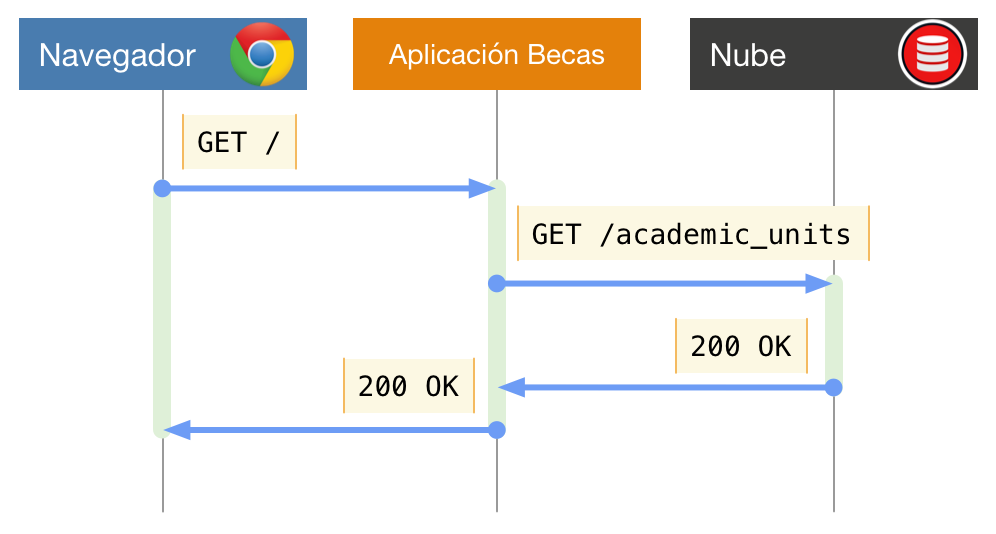
\includegraphics[width=\linewidth]{src/images/01-capitulo-1/ejemplo-rest-becas.png}
  \caption{Interacciones involucradas en el listado de becas por Unidad Académica}
  \label{fig:ejemplo-rest-becas}
\end{figure}

En la sección \ref{standard:rest} realizaremos el desarrollo pertinente de la definición de la arquitectura de aplicaciones distribuidas \gls{acro:rest} que Fielding publicó, dando de esa forma un marco teórico adecuado a las definiciones de nuestra nueva arquitectura para la nube de servicios.


\paragraph{El diseño final: el Integrador}

Luego de analizar las posibilidades que brindaba el uso de los principios \gls{acro:rest} en detalle, realizamos el primer diseño de cómo quedarían definidos los distintos servicios o \gls{term:endpoint} y decidimos darle un nombre: el \textit{Integrador}, una mezcla entre título de historieta\footnote{En cierto modo, nos recuerda historietas como Castigador (\eng{The Punisher}, de \eng{Marvel Comics}) – \url{https://es.wikipedia.org/wiki/Punisher}} y \eng{Terminator}, que nos acompaña hasta el día de hoy cuando hacemos referencia a la aplicación \textit{detrás} de la nube de servicios.

Realizando un enfoque más pragmático que correcto para el diseño, definimos servicios que retornan documentos \gls{lang:json} para cada una de las entidades que se podían consultar sin realmente analizar si serían realmente útiles, o si siquiera se accederían alguna vez. Fue de esta forma que la \gls{acro:api} se compuso de los más de 100 \gls{term:endpoint} que tiene hoy, que no siguen una misma línea en su diseño,  no tienen una estructura estándar de respuesta, y de los cuales efectivamente se usa tan solo el 46\%\footnote{Esta cifra surge de los datos que tenemos en nuestra herramienta de analíticas. De los 105 servicios que existen, 56 no registran accesos en el último año.}. En el \nameref{anexo:endpoints-nube-actual} listamos todos los servicios provistos por la nube para utilizar de referencia.

Sin entrar en detalles sobre cada \gls{term:endpoint}, el diseño existente muestra la falta de consistencia general en la definición de las \glspl{acro:url}, la sobrecarga de niveles de anidamiento en servicios como el que devuelve las materias del plan de estudios de una carrera de una Unidad Académica\footnote{\lstinline$/api/academic_unit/:id/career/:career_id/career_programme/:career_programme_id/career_subject.json$} que anida esos 3 niveles para mostrar la información, aunque los identificadores únicos de cada elemento podrían usarse, en una estructura más plana, para acceder directamente al último nivel, algo así como \lstinline$/api/career_programme/:career_programme_id/career_subject.json$ y así simplificar las \glspl{acro:url}.

Estos problemas sumados a la falta de documentación sobre cómo usar los diferentes servicios, qué parámetros reciben y qué estructura tiene la respuesta cada uno, hacen más complejo el uso de esta \gls{acro:api} tanto para desarrolladores que la venimos utilizando hace tiempo, como para nuevos integrantes del equipo a los que queremos sumar a alguna aplicación que haga uso de estos servicios.

\paragraph{El Integrador: implementación}

La nube de servicios, como aplicación, fue un desarrollo más realizado en PHP 5 y el framework \gls{fw:symfony} 1.4, utilizando MySQL como motor para las 5 bases de datos que utiliza para proveer la información:

\begin{itemize}
  \item Una base de datos donde se almacena información propia de la aplicación: tokens de acceso, estadísticas de acceso, información de clientes de la \gls{acro:api}.

  \item Una segunda base de datos para los datos de referencia de los que ya hemos hablado (tipos de documento, países, etcétera).

  \item Una tercera base en la que se mantiene actualizada la información que nos llega desde la oficina de Liquidaciones del CeSPI, la cual se transforma mediante procesos \gls{acro:etl}\footnote{Técnica que se utiliza para tomar datos de una o múltiples fuentes de información, modificarla y cargarla en una o más almacenes de datos. En nuestro caso utilizamos la herramienta Kettle de la versión de comunidad de la suite Pentaho para transformar los datos fuente, que nos llegan en archivos de texto plano, en inserciones normalizadas en nuestra base de datos MySQL.}\cite{paper:etl} para normalizarla antes de guardarla en esta base de datos.

  \item Una cuarta para la información que proviene de los SIU Guarani de las distintas Unidades Académicas, la cual es actualizada directamente por el grupo de Sistemas Académicos del {\cespi}.

  \item Y una quinta base de datos donde se unifican y mezclan los datos de las últimas 3 bases datos mencionadas, de manera tal que se logre una trazabilidad de la persona como un todo a lo largo de su \textit{vida en la UNLP}, ya sea como alumno, docente o no docente.
\end{itemize}

La aplicación se realizó sin considerar algunos aspectos claves para mejorar la \eng{performance} del lado de los clientes de la \gls{acro:api}, como puede ser utilizar cabeceras de \eng{caching}, compresión de respuestas, utilizar \eng{caches} compartidas y otras estrategias que desarrollaremos más en detalle como parte de nuestro análisis para el futuro de la nube de servicios.

Para las \gls{term:aplicacionessatelitales}, se realizó un \eng{plugin} de \gls{fw:symfony} que abstraía en clases y objetos la mayoría de los servicios existentes, implementando cierto mecanismo de \eng{caching} local a cada aplicación. Este mecanismo ayudó drásticamente a mejorar los tiempos de respuesta de las aplicaciones, con casos en que presentar una página al usuario tomaba alrededor de 20 segundos sin \eng{caching} y menos de 5 segundos con él. Pero por tratarse de decisiones realizadas meramente del lado de las aplicaciones cliente, existían situaciones en las que la información almacenada en esa \eng{cache} local quedaba desactualizada (\eng{stale}, en inglés) con respecto a lo que la \gls{acro:api} devolvía como el dato actual (\eng{fresh}, en inglés), por lo que en algunos casos se debió implementar un mecanismo manual de vaciado de \eng{cache} para subsanar estas situaciones.

En resumen: la implementación fue adecuada y funcional para las necesidades del momento, pero con el tiempo esas necesidades y, principalmente, la tecnología fueron cambiando, lo cual fue acrecentando gradualmente la necesidad de un nuevo análisis y replanteo para la solución actual.


\subsubsection{Cuarta iteración: este trabajo}
\label{nube:etapa4}

Mucha agua ha pasado bajo el puente desde que implementamos la versión actual de la nube de servicios de la UNLP, y varios han sido los cambios que el paso de estos 4 años nos ha dejado: pasamos de ser un equipo de alrededor de 8 personas en que todos nos dedicábamos a desarrollar aplicaciones web en PHP con el framework \gls{fw:symfony}, algunos toques de JavaScript para la interfaz de usuario y bases de datos MySQL, a ser un equipo de 17 personas que desarrolla aplicaciones en el lenguaje Ruby, con \gls{fw:rails} y \gls{fw:sinatra} como \eng{frameworks} web de cabecera, realizando algunas pequeñas aplicaciones meramente en JavaScript, que ha reescrito en Ruby varias de las aplicaciones realizadas en PHP y mantiene activamente aquellas desarrolladas en \gls{fw:symfony} que aún no se han migrado, utilizando bases de datos MySQL mayoritariamente y en algunos casos combinándolas con bases de datos \gls{db:nosql} y almacenes clave-valor en memoria, como \gls{db:redis} o \gls{db:memcached}. A modo de referencia, en el  \nameref{anexo:detalle-clientes} detallamos las aplicaciones que actualmente estamos manteniendo y desarrollando.

Estos cambios han traído aparejada la implementación de un cliente desarrollado en Ruby para integrarlo, de la misma forma que lo hicimos en el caso de las aplicaciones PHP, en las aplicaciones basadas en \gls{fw:rails} y \gls{fw:sinatra}. Este fue otro caso más donde las limitaciones del Integrador actual debieron ser sorteadas mediante la adición de lógica del lado del cliente:

\begin{itemize}
  \item Las aplicaciones cliente desarrolladas en Ruby implementan una cache condicional basada en \gls{db:redis} o en archivos del filesystem (según disponibilidad, y en ese orden de prioridad), que almacena las respuestas a los requerimientos por un tiempo determinado\footnote{La posibilidad de especificar el tiempo por el cual se desea guardar la copia en cache (el \gls{acro:ttl}) fue agregada recién en abril de 2015, es decir que antes se almacenaban indefinidamente las copias en \eng{cache}, lo que para los casos en que se usaba el sistema de archivos como almacenamiento esto representaba un potencial problema de crecimiento sin tope de los archivos utilizados para la cache.} e intenta subsanar la falta de directivas de cabeceras de parte de la \gls{acro:api} de servicios.

  \item Al no tener un estándar para la estructura de las respuestas, la lógica de hidratación de estos documentos \gls{lang:json} para convertirlos en objetos del dominio de las aplicaciones es excesivamente costosa en términos de \eng{performance} y tiene varios chequeos que podrían evitarse si se normalizaran y estandarizasen las respuestas.

  \item La falta de documentación nos ha obligado en ocasiones teniendo que hacer una suerte de ingeniería inversa de las respuestas para entender relaciones entre datos.
\end{itemize}

Otro gran problema es la dificultad para escalar que tiene la arquitectura actual. La aplicación web que atiende los pedidos a la nube y sus 5 bases de datos viven en una misma máquina virtual, lo cual puede ser hasta cierto punto conveniente para tener un mantenimiento y administración centralizados, pero esto acota en gran medida la posibilidad de poner rápidamente en funcionamiento nuevas instancias de la \gls{acro:api} que puedan balancear proporcionalmente la carga ante la creciente demanda que tiene por parte de las aplicaciones cliente. Este único punto de falla también es un potencial riesgo en caso de intrusiones o caídas de cualquier índole: fallas eléctricas, de red, de disco o errores humanos a la hora de realizar el mantenimiento de ese equipo virtual. Las tecnologías que utiliza ya no son mantenidas por sus desarrolladores: PHP 5.3 alcanzó su fin de mantenimiento (o \eng{end of life}, como la comunidad de PHP lo denomina) el 14 de agosto de 2014\footnote{Cf. \url{http://php.net/eol.php}} y \gls{fw:symfony} 1.4 dejó de ser mantenido en Noviembre de 2012\footnote{Cf. \url{http://symfony.com/blog/symfony-1-4-end-of-maintenance-what-does-it-mean}}, lo cual implica que en cierto modo la aplicación puede eventualmente ser víctima de nuevas vulnerabilidades que se descubran a esa rama del desarrollo y que ya no serán solucionadas.

Todos estos cambios y problemas motivan el presente trabajo, en el cual analizaremos las posibilidades que ofrece una \gls{acro:api} diseñada desde el comienzo con el nivel más alto\footnote{Así define Leonard Richardson el conjunto de requerimientos para alcanzar un servicio que cumpla realmente con todos los principios que Roy Fielding definió para una \gls{acro:api} \gls{acro:rest}, y define que \gls{acro:hateoas} es el requerimiento de nivel 3 para alcanzar la pureza de \gls{acro:rest}. – \url{http://www.crummy.com/writing/speaking/2008-QCon/act3.html} y claramente analizado por Martin Fowler en \url{http://martinfowler.com/articles/richardsonMaturityModel.html}} de adhesión a \gls{acro:rest} posible (\gls{term:hypermedia}), basándonos en estándares ya establecidos en lugar de intentar reinventar la rueda y definir el nuestro propio para las respuestas \gls{lang:json}, pensando en aprovechar las posibilidades de caching que ofrecen las distintas capas del diseño, e intentando descentralizar la información de manera tal que se elimine el único punto de falla que existe en la actualidad y que nos permita escalar horizontalmente en cantidad de instancias de la nube de manera transparente y poco costosa.


  %   - Capítulo II
  \section{Capítulo II}
\label{cap2}

\todo{Escribir una breve introducción para este capítulo}

\textit{En este capítulo se sentará un marco teórico para nuestra propuesta de trabajo.}

\subsection{Historia del procesamiento distribuido}
\label{soa:historia}

Los sistemas mainframe de las décadas de 1960 y 1970, como la serie IBM System/360, raramente se comunicaban entre sí, y cuando lo hacían el proceso de transferencia de información de un sistema a otro era realizado por medio de una cinta magnética. Con el tiempo y ante el creciente número de sistemas dentro de las organizaciones, el acceso en tiempo real entre éstos se hizo cada vez más necesario, tanto dentro de la misma organización como fuera de ella, como en el caso de los mercados financieros que requerían realizar transacciones en tiempo real.

Inicialmente, el acceso en tiempo real se lograba vía comunicaciones de socket de bajo nivel, usualmente escritas en lenguaje assembler o C, cuya programación era compleja y requería amplios conocimientos en los protocolos de redes. Luego entraron en escena protocolos como \gls{acro:nfs} y \gls{acro:ftp}, que permitieron abstraerse de la complejidad de los sockets definiendo mecanismos de comunicación que facilitaron el intercambio de información. Estos protocolos dieron pie a abstracciones con aún más posibilidades como \gls{acro:rpc}, un protocolo que permite realizar llamadas a funciones para que sean ejecutadas en un servidor remoto.

En la década de 1980 las computadoras personales habían entrado en escena y los desarrolladores estaban buscando formas más eficaces para aprovechar la potencia de cálculo de estos equipos. Asimismo, el número de servidores dentro de las organizaciones se incrementó exponencialmente debido a la disminución en el precio del hardware. Estas tendencias, junto con la creciente madurez de \gls{acro:rpc}, impulsaron dos importantes avances en la computación distribuida: \gls{acro:corba} y \gls{acro:dcom}, tecnologías que ofrecían herramientas para desarrollar aplicaciones distribuidas en entornos heterogéneos. Todas estas comunicaciones entre las organizaciones eran caras y dependían de líneas alquiladas con propósitos específicos que formaban circuitos privados, lo cual resultaba práctico solamente para las grandes empresas.

A finales de la década de 1990, con la extendida adopción de internet las compañías comenzaron a reconocer los beneficios de expandir sus plataformas digitales a socios y clientes, principalmente por la reducción de costos que este medio implicaba. Desafortunadamente, la utilización de \gls{acro:corba} o \gls{acro:dcom} para las comunicaciones en internet resultó ser todo un reto, en parte debido a las restricciones impuestas por los \eng{firewalls} que sólo permitían el tráfico \gls{proto:http} (necesario para los navegadores y comunicaciones con servidores web), y en parte porque ni \gls{acro:corba}, ni \gls{acro:dcom} lograron dominar el mercado.

Cuando el protocolo \gls{ws:soap} apareció por primera vez en enero de 2000, fue promocionado como la panacea debido a su dependencia interoperable en \gls{lang:xml}. \gls{ws:soap} fue concebido principalmente como una alternativa a \gls{acro:corba} y \gls{acro:dcom} para realizar llamadas remotas a procedimientos. En este sentido, vale la pena señalar que RPC SOAP era una mejora sobre las implementaciones \gls{acro:rpc} anteriores, ya que se basó en \gls{lang:xml} lo que facilitó un mayor grado de interoperabilidad entre los lenguajes de programación.

Si bien el procesamiento distribuido basado en \gls{acro:rpc} fue, sin duda alguna, una mejora sustancial sobre las comunicaciones basadas en sockets de bajo nivel, éste tenía varias limitaciones\cite[p.~6]{opensourcesoa:davis}:

\begin{itemize}
  \item La alta dependencia entre los sistemas locales y remotos requiere demandas de ancho de banda significativo, existiendo la posibilidad de que una excesiva cantidad de llamadas \gls{acro:rpc} de un cliente al servidor puedan generar una carga sustancial en la red.
  \item La naturaleza de grano fino de \gls{acro:rpc} requiere una red altamente predecible. En este sentido, la latencia impredecible, como es el caso de las comunicaciones sobre internet, es inaceptable para las soluciones basadas en \gls{acro:rpc}.
  \item La compatibilidad de tipos de datos de \gls{acro:rpc}, que tiene como objetivo proporcionar un soporte completo para todos los tipos de datos nativos (\texttt{array}, \texttt{string}, \texttt{integer}, etc.), se convierte en una complicación al tratar de compatibilizar lenguajes incompatibles, tales como C++ y Java.
\end{itemize}

Los mensajes RPC SOAP también sufrieron las mismas limitaciones inherentes como las mencionadas anteriormente. Afortunadamente, \gls{ws:soap} ofrece estilos de mensajes alternativos que superan estas deficiencias.

% se puede agregar mas del libro Open Source SOA - Advent of SOA - pp 7-8, hay un gráfico que esta bueno

\subsection{Arquitecturas Orientadas a Servicios}
\label{soa:definicion}

La Arquitectura Orientada a Servicios (\gls{acro:soa}) establece un marco de diseño para la integración de aplicaciones distribuidas e independientes, permitiendo acceder desde la red a sus funcionalidades que se ofrecen como servicio. Habitualmente \gls{acro:soa} es implementado mediante servicios web (\eng{Web Services}), tecnología basada en estándares e independiente de la plataforma que provee los datos, de esta manera \gls{acro:soa} puede descomponer las aplicaciones monolíticas en un conjunto de servicios\cite{microsoft2006}.

Existen varias definiciones de \gls{acro:soa}, muchas incluyen el término \eng{Web Service}, pero éstos conceptos no son lo mismo. \gls{acro:soa} es un paradigma y \eng{Web Service} es una forma posible de implementarlo.

Según Thomas Erl\cite{principlesofdesign:erl}, \gls{acro:soa} establece ``un modelo arquitectónico que tiene como objetivo mejorar la eficiencia, agilidad y productividad de una organización mediante la colocación de los servicios como el principal medio a través del cual se realizan los objetivos estratégicos asociados a la comunicación orientada a servicios''.

Para el Modelo de Referencia \gls{acro:oasis}, \gls{acro:soa} es un paradigma para organizar y utilizar capacidades distribuidas que pueden estar bajo el control de dominios diferentes.

\gls{acro:soa} incluye prácticas y procesos que se basan en el hecho de que los sistemas distribuidos no son controlados por los mismos propietarios. Diferentes equipos, departamentos, o incluso diferentes organizaciones pueden gestionar diferentes sistemas. Este concepto es clave para entender \gls{acro:soa} y grandes sistemas distribuidos.

En el pasado, se han propuesto una gran cantidad de métodos para resolver el problema de la integración de sistemas distribuidos mediante la eliminación de la heterogeneidad, pero sabemos que estos enfoques no funcionan. Los grandes sistemas distribuidos con diferentes propietarios son heterogéneos.  El enfoque \gls{acro:soa} acepta esta heterogeneidad, de manera similar a los métodos ``ágiles'' de desarrollo de software, que aceptan que los requisitos cambian en lugar de tratar de luchar contra esos cambios, \gls{acro:soa} acepta que existe una gran heterogeneidad en los grandes sistemas. No se puede introducir \gls{acro:soa} diseñando todo desde cero. Hay que lidiar con el hecho de que la mayoría de los sistemas legados que se encuentran en producción, se mantendrán\cite[p.~15]{josuttis2007}.

\subsection{Análisis de tecnologías SOA}
\label{soa:tecnologias}

\todo{Escribir el análisis de tecnologías SOA}

\subsubsection{Para los servicios}

\paragraph{Ruby on Rails}

\subparagraph{Rails + Grape}
\subparagraph{Rails API}

\paragraph{\gls{fw:sinatra}}


\subsubsection{Para la estructura de los servicios}

\paragraph{JSON-API}
\label{soa:tecnologias:json-api}


\subsubsection{Para la cache compartida}

\paragraph{Varnish}

\paragraph{Squid}
\label{soa:tecnologias:squid}


\subsubsection{Para nodo central (ex-ESB)}

\paragraph{Mulesoft ESB}
\label{soa:tecnologias:mulesoft-esb}

\paragraph{Apache Synapse ESB}
\label{soa:tecnologias:apache-synapse}

\paragraph{API Axle}

Ver $http://apiaxle.com$

\paragraph{Kong}
\label{soa:tecnologias:kong}

Es una herramienta desarrollada por la empresa Mashape que permite la fácil administración de \glspl{acro:api}, centralizando el acceso a las mismas desde uno o más servidores que se encargan de llevar registro de qué servicios ofrecen, recibir los requerimientos para éstos y delegar la generación de las respuestas a los \glspl{term:backend} destinados a tal fin.

Kong funciona con una versión modificada de \nameref{soa:tecnologias:nginx}, haciendo las de \eng{proxy} reverso y proveyendo una estructura extensible mediante el uso de agregados (\eng{plugins}) para brindar funcionalidad adicional a la básica, como ser autenticación, registro en logs, limitación de datos (\eng{rate limiting}), \eng{caching}, por nombrar algunos. Toda su información se almacena en una base de datos no relacional Apache Cassandra, altamente escalable por naturaleza.

Básicamente, Kong se ubica entre los clientes y las instancias vivas de las \glspl{acro:api}, recibiendo los requerimientos para luego de aplicar las reglas que se le hayan especificado, enviarlos al servicio que corresponda.

\subparagraph{Licencia}

Kong está publicado bajo licencia Apache 2.0\footnote{La misma puede ser consultada accediendo a \url{https://getkong.org/license/}}.

\subparagraph{Extensiones disponibles (\eng{plugins})}

Este producto permite extender su funcionalidad y comportamiento básico mediante la adición de \eng{plugins} que brindan variadas funciones. Adicionalmente, en caso que necesitemos agregar comportamiento que no se encuentra disponible, podemos implementarlo nosotros mismos y contribuir nuestro propia extensión a la comunidad.

A continuación presentamos un breve listado de las extensiones que Kong ofrece actualmente:

\begin{itemize}
  \item \textbf{Autenticación:} Kong provee \eng{plugins} para agregar autenticación a las \glspl{acro:api} mediante distintas estrategias:
  \begin{itemize}
    \item \textbf{Basic:} Autenticación mediante usuario y contraseña. \\
    \url{https://getkong.org/plugins/basic-authentication}
    \item \textbf{Key:} Autenticación mediante una clave de \gls{acro:api}. \\
    \url{https://getkong.org/plugins/key-authentication}
    \item \textbf{OAuth 2.0:} Autenticación mediante el protocolo OAuth 2.0. \\
    \url{https://getkong.org/plugins/oauth2-authentication}
    \item \textbf{\gls{acro:hmac}:} Permite autenticar la identidad del cliente (\eng{consumer}) mediante firmas \gls{acro:hmac} en los mensajes. \\
    \url{https://getkong.org/plugins/hmac-authentication}
    \item \textbf{\gls{acro:jwt}:} Provee autenticación mediante el uso del estándar JSON Web Tokens. \\
    \url{https://getkong.org/plugins/jwt}
  \end{itemize}

  \item \textbf{Seguridad:} Las siguientes extensiones de Kong proveen capas adicinales de seguridad a los servicios:
  \begin{itemize}
    \item \textbf{\gls{acro:acl}:} Agrega listas de control de acceso para limiter qué consumers pueden acceder a qué \glspl{acro:api}. \\
    \url{https://getkong.org/plugins/acl}
    \item \textbf{\gls{acro:cors}:} Permite que se realicen requerimientos desde distintos dominios con las limitaciones que impongamos, algo ideal para la implementación de clientes puramente desarrollados en JavaScript que corran por completo en el navegador de los usuarios. \\
    \url{https://getkong.org/plugins/cors}
    \item \textbf{\gls{acro:ssl}:} Agrega la posibilidad de establecer conexiones verificables mediante la inclusión de certificados \gls{acro:ssl} a los servicios que proveemos, tanto individual como globalmente, sin necesidad de hacerlo en cada uno de los puntos de acceso de las \glspl{acro:api}. \\
    \url{https://getkong.org/plugins/ssl}
    \item \textbf{Restricciones por dirección IP:} Posibilita manejar listas blancas y listas negras de direcciones IP que pueden realizar requerimientos a nuestros servicios. \\
    \url{https://getkong.org/plugins/ip-restriction}
  \end{itemize}

  \item \textbf{Control de tráfico:} Estas extensiones habilitan reglas de control sobre el tráfico entrante y saliente de nuestras \glspl{acro:api}:
  \begin{itemize}
    \item \textbf{Límite de tasa de consulta (\eng{Rate limiting}):} Permite limitar la cantidad de requerimientos que un cliente puede hacer a los servicios en un periodo de tiempo dado. \\
    \url{https://getkong.org/plugins/rate-limiting}
    \item \textbf{Límite de tasa de respuesta (\eng{Response rate limiting}):} Hace posible limitar la cantidad de respuestas que los servicios envían en un periodo de tiempo dado (aplica límites sobre el tráfico saliente). \\
    \url{https://getkong.org/plugins/response-rate-limiting}
    \item \textbf{Límite de tamaño de solicitud (\eng{Request size limiting}):} Bloquea aquellos requerimientos cuyo cuerpo exceda un límite que especifiquemos en su tamaño. \\
    \url{https://getkong.org/plugins/request-size-limiting}
  \end{itemize}

  \item \textbf{Analíticas y monitoreo:} Tal vez el punto con menos opciones que provee Kong, ya que posee un único \eng{plugin} que agregue funcionalidad en este aspecto:
  \begin{itemize}
    \item \textbf{Galileo:} Integra el servicio de analíticas y monitoreo de \glspl{acro:api} Galileo, una plataforma paga de \eng{Business Inteligence} desarrollada por Mashape, los creadores de Kong. \\
    \url{https://getkong.org/plugins/galileo}
  \end{itemize}

  \item \textbf{Transformaciones:} Mediante estas extensiones, podemos realizar modificaciones a las peticiones o las respuestas de un servicio cuando pasa por Kong:
  \begin{itemize}
    \item \textbf{Transformación de peticiones (\eng{Request transformer}):} Modifica la solicitud antes de enviarla al servicio correspondiente. \\
    \url{https://getkong.org/plugins/request-transformer}
    \item \textbf{Transformación de respuestas (\eng{Response tranformer}):} Altera la respuesta obtenida desde la \gls{acro:api} antes de enviarla al cliente del servicio. \\
    \url{https://getkong.org/plugins/response-transformer}
  \end{itemize}

  \item \textbf{Registro de eventos (\eng{Logging}):} Estos \eng{plugins} permiten escribir a logs de registro las solicitudes y respuestas que pasan por Kong mediante distintas estrategias:
  \begin{itemize}
    \item \textbf{TCP:} Envía la información al log mediante una conexión realizada con un servidor que habla el protocolo TCP. \\
    \url{https://getkong.org/plugins/tcp-log}
    \item \textbf{UDP:} Ídem anterior, excepto que usando protocolo UDP. \\
    \url{https://getkong.org/plugins/udp-log}
    \item \textbf{HTTP:} \eng{Plugin} similar a los anteriores, excepto que lo hace contra un servidor que habla el protocolo HTTP. \\
    \url{https://getkong.org/plugins/http-log}
    \item \textbf{Archivo (\eng{File}):} Escribe la información en archivo local al servidor de Kong. \\
    \url{https://getkong.org/plugins/file-log}
  \end{itemize}
\end{itemize}

\subparagraph{Instalación y prueba}

Basándonos en los pasos detallados en la guía oficial de Kong\footnote{\url{https://github.com/Mashape/docker-kong}} para su instalación y ejecución mediante Docker\footnote{Desarrollar el potencial de Docker y las posibilidades que abre desde el punto de vista tanto de desarrollo de aplicaciones como de administración de las mismas en producción merecería un capítulo entero. Debido a que esto excede el alcance del presente trabajo, nos limitaremos a definir a Docker como una herramienta que permite ejecutar servicios (de cualquier tipo) en ambientes livianos aislados basados en GNU/Linux, los cuales ya empaquetan el servicio y cualquier dependencia que éste pudiera tener. Docker corre sobre un sistema operativo base que soporte la tecnología de contenedores (\eng{containers}). Para mayor información, se puede consultar el sitio oficial de Docker: \url{https://www.docker.com/what-docker}}, realizamos pruebas de concepto para analizar la factibilidad de implementación de esta herramienta, las cuales resultaron altamente satisfactorias. A continuación, reproduciremos las pruebas realizadas en el ambiente local\footnote{De ahí que todas las referencias a servicios que en estos pasos se realizan son utilizando \url{http://localhost}}, indicando los comandos ejecutados y las salidas obtenidas (en general acotadas a los datos relevantes para el caso). Para sintetizar los pasos, omitiremos la preparación del ambiente Docker, aunque se podría resumir simplemente en instalar dicha herramienta en el equipo donde se ejecutarán los contenedores.

Para iniciar los dos servicios requeridos por Kong para su funcionamiento (Apache Cassandra y Kong mismo), ejecutamos la siguiente secuencia de comandos:

\bashfile{src/02-capitulo-2/tecnologias/nodo-central/code/kong/00-preparacion.sh}

Con el último comando comprobamos que el servicio está funcionando y que responde con la información de la instancia en ejecución, en formato \gls{lang:json}. Ahora que Kong está correctamente instalado y ejecutándose, podemos pasar a configurarlo y probar su funcionamiento.

Por defecto Kong atiende requerimientos en dos puertos diferentes:

\begin{itemize}
  \item \textbf{Puerto \texttt{8000}:} Aquí escucha la porción pública de Kong que funciona como proxy reverso de los servicios que registremos en él, proveyendo acceso a sus \glspl{acro:api}. A este puerto irán dirigidos todos los requerimientos de los clientes.
  \item \textbf{Puerto \texttt{8001}:} En este puerto Kong provee una \gls{acro:api} administrativa, mediante la cual se realizan todas las tareas de configuración y personalización de la herramienta. Esto implica varias cosas: por un lado, no necesitamos tener acceso por consola a los servidores donde corre el servicio de Kong, ya que simplemente con peticiones \gls{proto:http} basta para configurarlo; y por otro lado que necesitamos agregar políticas de seguridad adicionales para limitar el acceso a este puerto.
\end{itemize}

Teniendo esto en cuenta, procederemos a configurar una \gls{acro:api} de pruebas en Kong, utilizando el servicio online Mockbin\footnote{\url{http://mockbin.com}} que ofrece \glspl{term:endpoint} que imitan una \gls{acro:api} real para este tipo de situaciones.

\bashfile{src/02-capitulo-2/tecnologias/nodo-central/code/kong/01-agregar-mockbin.sh}

Una vez agregada una \gls{acro:api}, en nuestro caso lo más probable será que querramos limitar su acceso mediante políticas de seguridad. A tal fin, agregaremos autenticación mediante clave con el \eng{plugin} \textbf{Key} de Kong.

\bashfile{src/02-capitulo-2/tecnologias/nodo-central/code/kong/02-habilitar-key-auth.sh}

Con esta breve prueba de concepto, hemos comprobado que tanto la instalación como el uso de Kong son sencillos, lo cual lo hace un gran candidato para su utilización como nodo central de la nueva arquitectura de la nube de servicios de la \unlp.

\subparagraph{Integración con nuestro diseño}

\begin{figure}
  \includegraphics[width=\linewidth]{src/images/02-capitulo-2/tecnologias/kong/kong-arq.jpg}
  \caption{Esquema de integración de Kong en nuestra propuesta.}
  \label{fig:integracion-kong-arquitectura}
\end{figure}

En nuestra arquitectura, tendríamos inicialmente un balanceador de carga delante de un cluster de instancias de Kong (junto con su correspondiente cluster de bases Cassandra con al menos dos instancias en réplica) como fachada para todas las peticiones a los servicios de la nube, y detrás de este tendríamos las distintas aplicaciones que proveen los \glspl{term:endpoint} específicos. En caso de necesitar escalar, bastará con agregar más instancias al cluster de Kong y, de ser necesario, también al cluster de bases de datos Cassandra.

En su función de proxy reverso, este producto nos será de gran utilidad al transicionar de la nube actual a la que estamos diseñando en este trabajo: podríamos enrutar todas las peticiones del \eng{hostname} \texttt{api2.dataintegration.unlp.edu.ar} a los servicios de la nube anterior y dirigir a las \glspl{acro:api} de la nueva arquitectura aquellas que lleguen a \texttt{cloud.unlp.edu.ar}. De esta forma, la migración de las aplicaciones cliente a la nueva arquitectura sería gradual.

\subparagraph{Conclusión}

Kong es una excelente alternativa al uso de un \gls{acro:esb}, ya que es más liviano, sencillo de configurar y administrar, altamente extensible y personalizable, y cubre las necesidades que tenemos en cuanto a escalabilidad, transparencia, centralización de la gestión y portabilidad.

\paragraph{API Umbrella}

Copiar desde $https://github.com/ncuesta/tesis-md/blob/master/productos/api-management/api-umbrella/api-umbrella.md$ (\textbf{ya está analizado})

\paragraph{Tyk}
\label{soa:tecnologias:tyk}

Ver \url{https://tyk.io}


\subsubsection{Para balancear la carga}

\paragraph{Apache}

Ver \url{http://httpd.apache.org/docs/2.2/mod/mod_proxy_balancer.html}

\paragraph{NGINX}
\label{soa:tecnologias:nginx}


\subsubsection{Para documentar}

\paragraph{API Blueprint}

Ver $https://apiblueprint.org/$

\paragraph{RAML}

RESTful API Modeling Language

Ver $http://raml.org/$

\paragraph{Swagger}

Ver \url{http://swagger.io/}



\newpage

  %   - Capítulo III
  \section{Capítulo III: Análisis}
\label{cap3}

En el proceso de elaboración de nuestra propuesta para el rediseño de la nube de servicios evaluamos diferentes tecnologías y herramientas para las diferentes partes en ella involucradas. En esta sección explicaremos, a partir de lo que hemos documentado de ese análisis, las principales alternativas que consideramos para cada caso.

Con el fin de agrupar lógicamente las herramientas a partir de su objetivo, las separamos en seis categorías e incluimos una conclusión por categoría en la que nos definimos por una de esas alternativas para utilizarla en nuestra propuesta final.

\subsection{Para los servicios}
\label{soa:tecnologias:para-servicios}

Siendo la parte de la arquitectura que mayor desarrollo y mantenimiento de nuestra parte implicará, decidimos utilizar el lenguaje Ruby para implementar los servicios web por los siguientes motivos:

\begin{itemize}
  \item \textbf{Robustez sin sacrificio de la elegancia:} Con varias aplicaciones en producción desarrolladas en este lenguaje, hemos comprobado que es robusto y potente, pero también elegante y \textit{cómodo} de utilizar.
  \item \textbf{Agilidad:} Implementar aplicaciones en Ruby, dada la gran oferta de librerías y frameworks que posee, es realmente ágil y práctico.
  \item \textbf{Nuestra experiencia:} Hace más de 3 años que desarrollamos a diario aplicaciones, herramientas y scripts con este lenguaje, y en estos años no hemos hecho más que apreciar cada vez más las bondades que tiene.
\end{itemize}

Partiendo de esa base, tomamos los dos frameworks para desarrollo de aplicaciones web más consolidados y utilizados\footnote{Para realizar esta apreciación nos basamos en las investigaciones que hemos hecho en el pasado como parte de nuestro trabajo en el {\cespi} y en los datos que el sitio \eng{The Ruby Toolbox} provee: \url{https://www.ruby-toolbox.com/categories/web_app_frameworks}.} en el ámbito de Ruby como posibles opciones con las cuales implementar nuestros servicios web: Ruby on Rails y Sinatra.

En este apartado describiremos ambos frameworks comparativamente para concluir en la elección que hemos hecho para el presente trabajo.

\subsubsection{Ruby on Rails}
\label{soa:tecnologias:rails}

Ruby on Rails, o simplemente Rails, es \textit{el} framework open source para desarrollo de aplicaciones web del lenguaje Ruby. Con más de 10 años de madurez y evolución, se ha convertido en el estándar \textit{de facto} a la hora de considerar los cimientos sobre los cuales basar el desarrollo de una aplicación web, ya sea a pequeña, mediana o gran escala. Tan fuerte ha sido su influencia que frameworks de otros lenguajes lo han tomado como base en su diseño, siendo el caso más emblemático de estos el de la versión \texttt{1} del framework web para PHP Symfony.

\paragraph{Un framework, muchas librerías}

Es un framework que sigue el patrón de diseño \gls{acro:mvc}, que organiza en tres capas la lógica del dominio de una aplicación y ayuda a delimitar de manera clara las incumbencias y responsabilidades de cada una de esas capas. Junto con esta organización siguiendo buenas prácticas probadas a lo largo de sus vastos años de existencia, Rails guía a los desarrolladores en el uso de técnicas beneficiosas como la realización de pruebas sobre el código de las aplicaciones (técnica conocida como \eng{testing}), la organización clara y limpia del código, y el uso de librerías consolidadas. Esas librerías son lo que conforman internamente a Rails:

\begin{itemize}
  \item Un conjunto de extensiones al lenguaje que simplifican y mejoran su usabilidad: \texttt{ActiveSupport}.
  \item Una capa de abstracción que permite manejar el modelo (la \textit{M} de \gls{acro:mvc}, datos y lógica de negocios) con y sin bases de datos: \texttt{ActiveRecord} y \texttt{ActiveModel}.
  \item Los controladores (la \textit{C} de \gls{acro:mvc}) que se encargan de aceptar y tratar los requerimientos entrantes a la aplicación, teniendo en cuenta aspectos importantes de seguridad, y de obtener la información necesaria para generar las respuestas: \texttt{ActionController} (parte de \texttt{ActionPack}).
  \item Un potente motor de generación de vistas (la \textit{V} de \gls{acro:mvc}) que permite generar código \gls{lang:html}, \gls{lang:json} o \gls{lang:xml} entre otros, para ser enviado en las respuestas a los clientes: \texttt{ActionView} (parte de \texttt{ActionPack}).
  \item Una serie de componentes adicionales que permiten realizar tareas comunes en las aplicaciones web, como el envío de correos electrónicos, comunicaciones mediante \eng{Web Sockets}, o el manejo de trabajos en segundo plano: \texttt{ActionMailer}, \texttt{ActionCable} y \texttt{ActiveJob}.
\end{itemize}

Rails integra estas librerías de manera tal que el desarrollo de la aplicación es ágil y se centra en la implementación de su lógica en sí, ya que el framework elimina decisiones triviales respecto a cómo organizar y gestionar elementos básicos comunes a cualquier aplicación web. Ese es otro gran punto a favor a la hora de ponderar Ruby on Rails y otras opciones.

\paragraph{El costo de Rails}

Ruby on Rails es una herramienta altamente potente y estable, pero que posee una contra respecto a otras opciones: su uso puede traer aparejadas penalizaciones en el rendimiento de nuestra aplicación. Para casos muy sencillos, con dominios muy reducidos, el uso de Rails puede llegar a ser contraproducente debido al \eng{overhead} que puede agregar la gran cantidad de componentes que posee. Podemos tomar como ejemplo nuestra situación: necesitamos realizar aplicaciones web para proveer los servicios de nuestra nube, por lo cual no utilizaremos partes comunes a una aplicación web tradicional como pueden ser el manejo de sesiones de los clientes, la generación de vistas en otros formatos que no sean \gls{lang:json}, el envío de correos electrónicos\footnote{En general no será utilizado, aunque tenemos planes de implementar un servicio de notificaciones que sí lo haría.}, por nombrar algunos. Para situaciones como la nuestra, en general se suele optar por otros frameworks con funcionalidad más reducida, que eliminan ese \eng{overhead} que agrega Rails, por lo que en nuestro caso sería contraproducente la utilización de éste. O al menos lo era, hasta la versión \texttt{4.2}.

\paragraph{\texttt{rails --api}}

En su versión \texttt{5.0} (la versión más reciente al momento de escritura del presente trabajo), Ruby on Rails  incorpora un nuevo \textit{modo} de creación de aplicaciones web: el modo \texttt{--api}. Esto permite iniciar aplicaciones configuradas con un subconjunto reducido de componentes, obtenido a partir de la eliminación de aquellos que no son necesarios para el desarrollo de \glspl{acro:api} web, y preparadas para servir contenido en formato \gls{lang:json} por defecto, aprovechando las técnicas de caching principales para este tipo de aplicaciones.

\paragraph{Sinatra}
\label{soa:tecnologias:sinatra}

Sinatra, más que un framework, es un \gls{acro:dsl} simple para el desarrollo rápido de aplicaciones web. Comparado con un framework completo como \nameref{soa:tecnologias:rails}, Sinatra ofrece un conjunto reducido de funcionalidad, el estrictamente necesario para implementar la vista y el controlador del patrón \gls{acro:mvc}, pero no soporta oficialmente una forma concisa de organizar la lógica de negocios de las aplicaciones (la \textit{M} de \gls{acro:mvc}).

Su mayor fortaleza radica en que permite rápidamente implementar aplicaciones web sencillas agregando un \eng{overhead} mínimo. Podemos implementar una aplicación que reciba peticiones y responda con documentos \gls{lang:html} o \gls{lang:json} en poco tiempo y con muy pocas líneas de código, pero a medida que la complejidad crece es necesario complementar Sinatra con otras librerías de manera manual, lo cual no hace de esta herramienta un candidato fuerte para solucionar nuestras necesidades al implementar los servicios de la nube de la \unlp. Por ejemplo, si deseamos implementar modelos con conexión a una base de datos seguramente agreguemos \texttt{ActiveRecord}, la capa de abstracción de \nameref{soa:tecnologias:rails}, y en el proceso deberemos manejar nosotros mismos la configuración y lógica de conexión a esa base de datos; similarmente ocurrirá si necesitamos utilizar una base de datos en memoria para el caching de nuestras aplicaciones (como podría ser \gls{db:redis} o \gls{db:memcached}).

\subparagraph{Sencillez compleja}

En el pasado hemos utilizado Sinatra para implementar algunas aplicaciones web sencillas, principalmente orientadas a proveer \glspl{acro:api} que den soporte a clientes para mostrar datos a los usuarios. En esa experiencia comprobamos lo sencillo que es implementar aplicaciones pequeñas con esta herramienta, lo cual es altamente beneficioso para desarrolladores experimentados así como para aquellos que no lo son. Tiene un conjunto claro de directivas, una documentación extensa y detallada traducida al español, y promueve el desarrollo ágil y conciso.

También nos encontramos con los inconvenientes que trae aparejado Sinatra a la hora de salir de la \textit{zona de comfort} de la herramienta: como mencionamos anteriormente, el trabajo adicional que requiere utilizar bases de datos, enviar correos electrónicos o implementar técnicas de caching, es un \eng{overhead} no funcional que afecta en gran medida el desarrollo de las aplicaciones, quitando tiempo útil para destinarlo en tomar decisiones triviales que no afectan funcionalmente a las aplicaciones. Al ser tan sencillo, Sinatra tampoco promueve una forma estándar de organizar el código, lo cual es propenso a decisiones tendenciosas por parte de cada desarrollador a la hora de ubicar los componentes lógicos de la aplicación, resultando en muchos \textit{pseudo-estándares} conviviendo en un mismo proyecto.

\subsubsection{Conclusión}
\label{soa:tecnologias:apps:conclusion}

Al analizar estas dos opciones decidimos realizar una pequeña prueba de concepto implementando una parte de la \gls{acro:api} de datos de referencia en \nameref{soa:tecnologias:rails} y en \nameref{soa:tecnologias:sinatra}. Esto no sólo nos permitió comparar el rendimiento de ambas versiones en términos de sus tiempos de respuesta, si no que además pudimos contrastar el esfuerzo necesario para desarrollar la misma solución en los dos contextos.

\paragraph{En términos de \eng{performance}}

Desde una visión estrictamente numérica ambas alternativas se comportaron de manera similar, obteniendo tiempos de respuesta promedio por debajo de los \textbf{\texttt{150} milisegundos} en general. Al habilitar la cache local y las cabeceras de caching en el caso de la implementada con \nameref{soa:tecnologias:rails}, las respuestas aprovechando esos niveles de cache bajaron al orden de los \textbf{\texttt{10} ó \texttt{20} milisegundos}, lo cual fue un gran salto de velocidad de respuesta.

Si bien nos fue de gran utilidad implementar estas pruebas de concepto, desde el punto de vista de la \eng{performance} estrictamente no existe una diferencia determinante que indique claramente qué herramienta utilizar. Es por esto que debemos considerar otro enfoque para la comparación: el de la productividad del desarrollador.

\paragraph{Desde el punto de vista del desarrollador}

Además de su rendimiento, otro factor importante a la hora de elegir un framework para el desarrollo es tener una noción de en qué medida agiliza y facilita la implementación de la aplicación propiamente dicha. Algunos casos en que la herramienta podría impactar negativamente en el desarrollo son:

\begin{itemize}
  \item Si el desarrollador se ve obligado a tomar decisiones no funcionales muy seguido,
  \item si el framework necesita ser complementado con un número alto de librerías de terceros para cubrir los requerimientos,
  \item si extender la funcionalidad del framework implica mucha investigación y trabajo manual, o
  \item si simplemente el conjunto de funcionalidad que éste ofrece no es suficiente.
\end{itemize}

Cualquiera de estas situaciones que enumeramos a modo de ejemplo funciona como indicador de que la herramienta elegida no está a la altura de las circunstancias, y eso fue exactamente lo que nos ocurrió al implementar la prueba de concepto con \nameref{soa:tecnologias:sinatra}. Nos encontramos con la necesidad de implementar y gestionar manualmente la conexión a la base de datos, con la falta de organización clara del código del proyecto, y con una complejidad innecesaria para implementar técnicas de caching.

Por el contrario, al implementar la prueba de concepto con \nameref{soa:tecnologias:rails} no existieron estos retrasos en el desarrollo. El posible inconveniente que puede existir al adoptar Rails como framework para el desarrollo es la curva de aprendizaje del mismo, pero en nuestro caso no es un factor a considerar debido a que ya poseemos experiencia con él tanto nosotros como el resto de nuestro equipo de trabajo. El desarrollo de esa prueba de concepto fue mucho más ágil que en el caso de \nameref{soa:tecnologias:sinatra} y prácticamente no tuvimos que tomar decisiones triviales o considerar cómo organizar el código del proyecto, ya que el mismo framework nos facilitaba esas decisiones.

Por esas razones es que hemos optado por usar el framework \nameref{soa:tecnologias:rails} como base para el desarrollo de los servicios de la nueva versión de la nube de la UNLP.


\subsection{Para la estructura de los servicios}
\label{soa:tecnologias:para-estructura}

La consistencia, coherencia y claridad en la estructura de las respuestas de los servicios que una nube provee es crítica para su usabilidad y mantenibilidad. En el diseño del Integrador hemos optado por definir nuestra propia estructura basada simplemente en el esquema de nuestras bases de datos: publicamos todos los campos indiscriminadamente, lo cual resulta en algunos casos en la exposición innecesaria y excesiva de valores en las respuestas de la \gls{acro:api}. Esto, sumado a una cierta inconsistencia en los nombres de los campos y en la forma en que se conforman las \glspl{acro:url} y sus parámetros, hacen difícil el uso de la nube sin consultas constantes a una documentación incompleta y desactualizada; consultas que en la myoría de los casos acaban por convertirse en una pérdida de tiempo y en la necesidad de leer el código fuente de las \glspl{acro:api} para conocer exactamente qué parámetros admite y qué efecto tienen en la petición.

En nuestro análisis de la nube actual éste fue uno de los puntos más importantes a mejorar: el requerimiento de tener una estructura estandarizada, fundada en casos de éxito, y que se integre con alguna herramienta de automatización de la documentación (veremos más sobre eso en la \autoref{soa:tecnologias:para-documentar}) para que podamos tenerla actualizada sin necesidad de hacerlo manualmente.

Con respecto al formato de la respuestas, hemos decidido mantener \gls{lang:json} como nuestra opción. Se trata de un formato muy amistoso para el desarrollador por su claridad y su relativamente poco \eng{overhead} para la codificación y decodificación, además de que se encuentra en uso en un creciente número de \glspl{acro:api} a nivel global\footnote{El interés en las \glspl{acro:api} \gls{lang:json} ha crecido constantemente desde el año 2004 al presente según las tendencias de Google. Cf. \url{http://www.google.com/trends/explore?q=xml\%20api\%2C\%20json\%20api\%2C\%20html\%20api}.}, por lo que nos centramos en la búsqueda de estándares específicos al formato \gls{lang:json}.

En este apartado analizaremos diferentes estándares, relacionados a la estructura de las respuestas y parámetros en las consultas, para el diseño y la implementación de una \gls{acro:api}.

\paragraph{HAL}
\label{soa:tecnologias:hal}


Ver \url{http://stateless.co/hal_specification.html}

\subsubsection{JSON API}
\label{soa:tecnologias:json-api}

JSON API es una especificación surgida en 2013 que intenta definir tanto cómo deben los clientes formular las peticiones, así como la forma en que los servidores deben responder a ellas, fomentando la eficiencia en el uso de recursos. Al momento de escritura del presente trabajo, esta especificación se encuentra en su versión \texttt{1.0} y con una versión \texttt{1.1} en proceso de definiciones.

En este análisis resumiremos de manera concisa los puntos sobresalientes de la especificación.

\paragraph{\eng{Media type} dedicado}

Tanto los datos que el cliente envía en su petición como la respuesta del servidor deben indicar el \eng{media type} dedicado de JSON API: \texttt{application/vnd.api+json}\footnote{Este tipo de contenido fue asignado por la IANA - \url{http://www.iana.org/assignments/media-types/application/vnd.api+json}}.

Este tipo de contenidos es una definición de estructura basada en el lenguaje \gls{lang:json}. Denominaremos ``documentos JSON API'' a aquellos documentos \gls{lang:json} que adhieran a este \eng{media type}.

\paragraph{Estructura general de los documentos JSON API}

Los documentos deben contener como elemento raiz un objeto, en el cual son admisibles las siguientes propiedades de primer nivel:

\begin{itemize}
  \item \texttt{data}: la información principal del documento, puede ser un recurso o una colección de éstos.
  \item \texttt{errors}: indicadores de cualquier error que hubiera ocurrido.
  \item \texttt{meta}: especifica metadatos sobre la información.
  \item \texttt{jsonapi}: descripción de la implementación del servidor JSON API.
  \item \texttt{links}: conjunto de vínculos hypermedia relacionados a la información principal.
  \item \texttt{included}: recursos incluidos en el documento por estar relacionados al objeto principal.
\end{itemize}

\paragraph{Los recursos}

Los elementos principales de información de un documento JSON API son los recursos. Cada recurso debe al menos tener dos propiedades: \texttt{id} y \texttt{type}, excepto cuando se trate de un \textit{nuevo} elemento que esté siendo creado por el cliente del servicio en cuyo caso el \texttt{id} puede omitirse. Además de estas propiedades obligatorias un recurso puede tener las propiedades \texttt{attributes}, \texttt{relationships}, \texttt{links} y \texttt{meta}, donde las dos primeras son objetos \gls{lang:json} que indican los atributos del recurso y posibles elementos relacionados respectivamente, y las últimas dos tienen sentidos similares a las propiedades homónimas del elemento raiz mencionadas en el apartado anterior que describe la estructura general de un documento JSON API. En el mismo sentido, los recursos pueden identificarse mediante una versión reducida de sí mismos que sólo contenga las propiedades \texttt{id} y \texttt{type}, caso en el cual se los denomina ``objetos identificadores de recursos''.

En este punto, la especificación hace una recomendación respecto de los campos (dentro de los \texttt{attributes} de un recurso) que representan \textit{asociaciones lógicas} o claves foráneas a otros recursos: los valores de clave foránea apuntando hacia otros recursos no deberían aparecer entre los atributos del recurso; en cambio debieran tener su entrada dedicada entre las \textit{relationships} del mismo.

Las relaciones de un recurso son objetos \glspl{lang:json} que pueden tener las siguientes propiedades:

\begin{itemize}
  \item \texttt{links}: un objeto \glspl{lang:json} que puede tener dos propiedades, \texttt{self} (\gls{acro:url} mediante la cual se puede manipular la relación en sí) y \texttt{related} (\gls{acro:url} del recurso asociado en sí, que no debe ser dependiente de la existencia de la relación).
  \item \texttt{data}: uno o varios (acorde a la cardinalidad de la relación) objetos identificadores de recursos para los recursos asociados.
  \item \texttt{meta}: un objeto \glspl{lang:json} con metadatos sobre el recurso.
\end{itemize}

La especificación, con miras a hacer un uso más eficiente de los recursos, define también los ``documentos compuestos'' que son aquellos que incluyen en la misma estructura la información relacionada a los recursos asociados a la información principal del documento, es decir, aquellos recursos referenciados en alguna de las relaciones. La información de estos recursos adicionales debe realizarse dentro de una clave \texttt{included} de primer nivel en la raiz del documento JSON API. Al incorporar esta información adicional al documento, se reducen la cantidad de peticiones necesarias para obtener un recurso y sus elementos relacionados, reduciendo la utilización de recursos necesaria para completar la tarea.

\jsonfile{src/03-capitulo-3/tecnologias/estructura/code/json-api/recurso.json}
\captionof{listing}{Documento JSON API representando un recurso\label{soa:tecnologias:json-api:recurso}}

\paragraph{Obtención de recursos}

Las peticiones de acceso de lectura a la información deben ser realizadas utilizando el método \gls{proto:http} \texttt{GET} y utilizando alguna de las \glspl{acro:url} provistas en los documentos JSON API como vínculos \texttt{self} o \texttt{related}. Por ejemplo, las peticiones presentadas a continuación son válidas para obtener información a partir del documento JSON API presentado anteriormente.

Esta petición se puede utilizar para obtener la colección de tipos de documentos:

\begin{listing}[H]
  \httpfile{src/03-capitulo-3/tecnologias/estructura/code/json-api/obtener-coleccion.http}
  \caption{Petición de una colección de recursos JSON API}
  \label{soa:tecnologias:json-api:obtener-colecccion}
\end{listing}

Esta otra para obtener todas las personas relacionadas con el tipo de documento con \texttt{id} \texttt{"0"}:

\begin{listing}[H]
  \httpfile{src/03-capitulo-3/tecnologias/estructura/code/json-api/obtener-recurso-relacionado.http}
  \caption{Petición de un recurso relacionado en JSON API}
  \label{soa:tecnologias:json-api:obtener-recurso-relacionado}
\end{listing}

Y la siguiente para obtener una persona en particular:

\begin{listing}[H]
  \httpfile{src/03-capitulo-3/tecnologias/estructura/code/json-api/obtener-recurso.http}
  \caption{Petición de un recurso en JSON API}
  \label{soa:tecnologias:json-api:obtener-recurso}
\end{listing}

Las respuestas exitosas a estas peticiones deben devolver un código de estado \gls{proto:http} \texttt{200 OK} junto con el recurso (o un elemento nulo, en caso de no existir el recurso identificado y estar siendo solicitado a través de una relación) o la colección de recursos (o una colección vacía, en caso de no poseer elementos). En el caso de las peticiones para obtener un único recurso inexistente que no sean realizadas a través de la \gls{acro:url} de una relación, el servidor deberá responder con un código de estado \gls{proto:http} \texttt{404 Not Found}.

El documento JSON API expuesto en el bloque de código \autoref{soa:tecnologias:json-api:recurso} es un ejemplo del cuerpo de una respuesta exitosa que debiera responder con el siguiente encabezado \gls{proto:http}:

\begin{listing}[H]
  \httpfile{src/03-capitulo-3/tecnologias/estructura/code/json-api/respuesta-200-ok.http}
  \caption{Encabezado HTTP de respuesta exitosa JSON API}
  \label{soa:tecnologias:json-api:respuesta-200-ok}
\end{listing}

Similarmente, el extracto presentado en el bloque de código \autoref{soa:tecnologias:json-api:respuesta-200-obtener-coleccion} representa una respuesta exitosa a una petición sobre la colección de tipos de documento.

\begin{listing}
  \httpfile{src/03-capitulo-3/tecnologias/estructura/code/json-api/respuesta-200-obtener-coleccion.http}
  \caption{Respuesta exitosa a petición de una colección de recursos en JSON API}
  \label{soa:tecnologias:json-api:respuesta-200-obtener-coleccion}
\end{listing}

Si en cambio la petición fuese exitosa pero su respuesta no contuviese elementos, las respuestas serían las presentadas en los bloques de código \autoref{soa:tecnologias:json-api:respuesta-200-recurso-nulo} (para un recurso singular) y \autoref{soa:tecnologias:json-api:respuesta-200-coleccion-vacia} para una colección.

\begin{listing}
  \httpfile{src/03-capitulo-3/tecnologias/estructura/code/json-api/respuesta-200-recurso-nulo.http}
  \caption{Respuesta JSON API para una petición exitosa a un recurso no encontrado}
  \label{soa:tecnologias:json-api:respuesta-200-recurso-nulo}
\end{listing}

\begin{listing}
  \httpfile{src/03-capitulo-3/tecnologias/estructura/code/json-api/respuesta-200-coleccion-vacia.http}
  \caption{Respuesta JSON API para una petición exitosa a una colección de recursos vacía}
  \label{soa:tecnologias:json-api:respuesta-200-coleccion-vacia}
\end{listing}

En los ejemplos anteriores se demuestra el uso del valor nulo (\texttt{null}) y la colección vacía (\texttt{[]}) para denotar la respuesta a una petición exitosa pero que no arroja coincidencias.

\paragraph{Obtención de relaciones}

Como se mencionó anteriormente, las relaciones pueden tener un vínculo a sí mismas (\texttt{self}) que permita manipular la relación en sí y no a los recursos que ésta vincula. Esa \gls{acro:url} consultada con el método \gls{proto:http} \texttt{GET} nos permite consultar la información asociada a esa relación, obteniendo como dato principal el recurso o los recursos involucrados en ella en forma de identificadores de recursos (objetos \gls{lang:json} con las propiedades \texttt{id} y \texttt{type} únicamente).

El servidor responderá con un código de estado \gls{proto:http} \texttt{200 OK} en caso de tratarse de una consulta exitosa, y con un \texttt{404 Not Found} si se tratase de una petición a una relación sobre un recurso principal inexistente.

\begin{listing}
  \httpfile{src/03-capitulo-3/tecnologias/estructura/code/json-api/respuesta-200-obtener-relacion.http}
  \caption{Respuesta JSON API para una petición exitosa a una relación}
  \label{soa:tecnologias:json-api:respuesta-200-obtener-relacion}
\end{listing}

\paragraph{Inclusión de recursos relacionados}

\todo{Completar spec de JSON API}
% Una forma interesante de aproximarse al problema de \eng{N + 1}

\subsubsection{Conclusión}

En nuestra búsqueda de formatos estándares para la estructura de la respuestas de nuestros servicios encontramos una gran variedad de opciones informales, propuestas desarrolladas por distintas empresas, pero sólo hallamos dos opciones que poseen la orientación adecuada para nuestras necesidades: \nameref{soa:tecnologias:hal} y \nameref{soa:tecnologias:json-api}.

El primer formato, \nameref{soa:tecnologias:hal}, es conciso y sencillo de implementar ya que no presenta grandes complicaciones en cuanto a sus requisitos funcionales. Si bien esto puede ser positivo, en esta situación nos resulta insuficiente para definir por completo el protocolo de acceso a nuestros servicios. En el mismo sentido, \nameref{soa:tecnologias:hal} no se encuentra en una versión definitiva, completa ni estable, lo cual lo elimina como candidato si consideramos que desde el año 2013 no recibe actualizaciones.

En el caso de \nameref{soa:tecnologias:json-api}, lo encontramos altamente beneficioso desde el punto de vista del desarrollo por su clara documentación, por tratarse de un estándar que define un protocolo de acceso a la información, por estar basado en las opiniones de varias empresas y equipos encabezados por arquitectos de renombre en la industria\footnote{Los principales editores de la especificación son Steve Klabnik (Ruby on Rails, lenguaje Rust), Yehuda Katz (Ruby on Rails, Ember.js, W3C TAG), entre otros.\\\url{http://jsonapi.org/about}}, por poseer una creciente adopción y por ser fácil de integrar con el framework que hemos elegido para implementar los servicios (\nameref{soa:tecnologias:rails}), y es por estos motivos que lo utilizaremos para estructurar las respuestas de nuestra nube de servicios.


\subsection{Para la cache compartida}
\label{soa:tecnologias:para-cache-compartida}

\subsubsection{Varnish}
\label{soa:tecnologias:varnish}

\gls{db:varnish} es un proxy reverso HTTP, a veces referenciado como HTTP accelerator o a \eng{web accelerator}, que almacena archivos y fragmentos de archivos en memoria, lo que reduce el tiempo de respuesta y el ancho de banda de red para las mismas solicitudes.\cite[p.~20]{varnish2016}

El proyecto Varnish fue iniciado por Verdens Gang en el 2005, contó con la gerencia, infraestructura y desarrollos adicionales aportados por la comunidad Noruega de Linux, que más tarde pasó a una empresa independiente, Varnish Software bajo licencia BSD.

Como mencionamos anteriormente, \gls{db:varnish} es un acelerador de aplicaciones web, que se instala delante de cualquier servidor HTTP y se configura para almacenar en la caché del servidor una copia del recurso solicitado. Pensado para mejorar el rendimiento de aplicaciones web con contenidos pesados y APIs altamente consumidas, éste será nuestro caso.

\begin{figure}[H]
  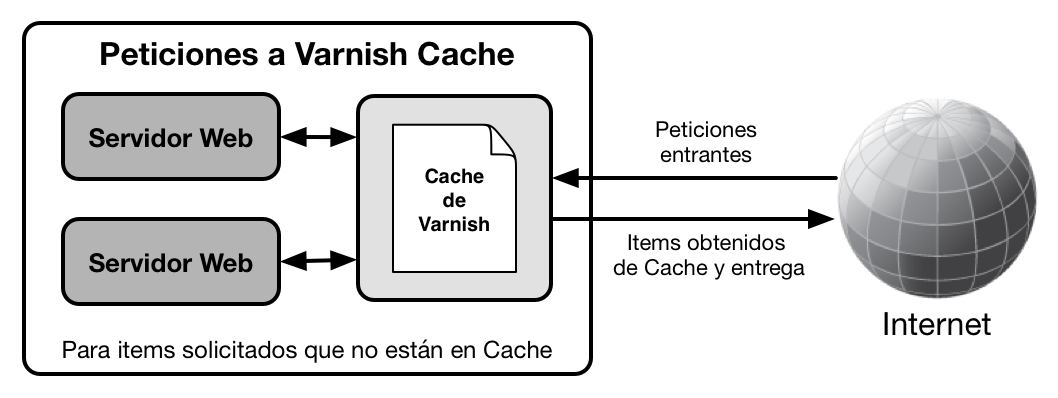
\includegraphics[width=\linewidth]{src/images/03-capitulo-3/tecnologias/varnish/varnish-reverse-proxy.png}
  \caption{Varnish Reverse Proxy}
  \label{fig:varnish}
\end{figure}

\paragraph{Instalación}

Varnish se distribuye en los respositorios de paquetes de Ubuntu, pero puede suceder que el paquete se encuentre desactualizado por lo tanto se recomienda usar los respositorios de paquestes de \url{varnish-cache.org}.

Para usar los respositorios de \url{varnish-cache.org} e instalar Varnish en Ubuntu 14.04, debemos ejecuatar la secuencia de comandos del bloque de código \autoref{soa:tecnologias:varnish-cache:bash-preparacion}:

\begin{listing}[H]
  \bashfile{src/03-capitulo-3/tecnologias/cache/code/varnish/00-preparacion.sh}
  \caption{Instalación de Varnish}
  \label{soa:tecnologias:varnish-cache:bash-preparacion}
\end{listing}

\subsubsection{Squid}
\label{soa:tecnologias:squid}

\gls{db:squid} es un proxy cache para la Web soporta \gls{proto:http}, \gls{proto:https}, \gls{acro:ftp}, entre otros. Reduce el ancho de banda y mejora los tiempos de respuesta por el almacenamiento en caché y la reutilización de las páginas web solicitadas frecuentemente.  Se ejecuta en la mayoría de los sistemas operativos disponibles, incluyendo Windows y está disponible bajo la GNU GPL.

\gls{db:squid} es usado por cientos de proveedores de internet en todo el mundo, para proporcionar a sus usuarios el mejor acceso posible a la web.  Optimiza el flujo de datos entre el cliente y el servidor, utilizando el contenido en caches frecuentemente usado, ahorrando de esta manera ancho de banda y obteniendo mejoras en el rendimiento de los clientes.

ver RFC 2186: Internet Cache Protocol (ICP), version 2
ver http://www.ietf.org/rfc/rfc2186.txt

Website Content Acceleration and Distribution
Thousands of web-sites around the Internet use Squid to drastically increase their content delivery. Squid can reduce your server load and improve delivery speeds to clients. Squid can also be used to deliver content from around the world - copying only the content being used, rather than inefficiently copying everything. Finally, Squid's advanced content routing configuration allows you to build content clusters to route and load balance requests via a variety of web servers.

\paragraph{Licencia}

\paragraph{Características principales}

\paragraph{Instalación y prueba}

\begin{listing}[H]
  \bashfile{src/03-capitulo-3/tecnologias/cache/code/squid/00-preparacion.sh}
  \caption{Instalación de Squid}
  \label{soa:tecnologias:squid-cache:bash-preparacion}
\end{listing}

\paragraph{Integración con nuestro diseño}

\subsubsection{Conclusión}

A continuación se detallan algunas de las ventajas de \gls{db:varnish} por sobre \gls{db:squid}:

\begin{itemize}
  \item Poul-Henning Kamp explica en \cite{website:www.varnish-cache.org} que \gls{db:varnish} delega en el kernel la administración de la memoria virtual, mientras que \gls{db:squid} intenta mantener separados el almacenamiento en disco y la memoria cache, lo que genera conflictos acerca de lo que debe paginarse a disco.

  \item Mejor performance y escalabilidad, \gls{db:squid} corre como un único proceso en un core de CPU, mientras \gls{db:varnish} utiliza un hilo (\eng{thread}) para cada cliente.

  \item \gls{db:varnish} utiliza VCL (\eng{Varnish Configuration Language}), que es un potente lenguaje de configuración que permite definir políticas de \eng{caching}, las mismas luego serán traducidas a código C, para más tarde ser compiladas.  Sin embargo, con \gls{db:squid}, algunas configuraciones resultan demasiado complejas, otras incluso no pueden realizarse.

  \item Actualmente \gls{db:varnish} es utilizado por una gran cantidad de sitios web con alta demanda de tráfico como pueden ser: The New York Times, The Guardian, The Hindu, sitios de redes sociales y contenidos como: Wikipedia, Facebook, Twitter, Vimeo, Tumblr, entre otros.

  \item Squid no soporta ESI o invalidaciones explícitas.

  \item Squid es un \eng{forward proxy} que puede ser configurado como \eng{reverse proxy}, mientras que Varnish es un \eng{reverse proxy}.
\end{itemize}

Además de las ventajas mencionadas anteriormente, el equipo de desarrollo del {\cespi} cuenta con la experiencia necesaria en la utlización de \gls{db:varnish}, ya que actualmente se encuentra implementado en producción para desarrollos realizados para la Universidad.  Por lo tanto, para nuestra implementación se instalará \gls{db:varnish} delante del balanceador de carga y de las instancias replicadas en las que se encuentran las diferentes \glspl{acro:api}, de esta manera, los accesos recurrentes a los mismos \eng{endpoints}, serán obtenidos desde la cache de \gls{db:varnish}, en lugar de acceder a cualquiera de las APIs, logrando obtener mejores tiempos de respuesta.


\subsection{Para el nodo central}
\label{soa:tecnologias:para-nodo-central}

\subsubsection{Mulesoft ESB}
\label{soa:tecnologias:mulesoft-esb}

Mule ESB es un \gls{acro:esb} liviano basado en Java, una plataforma de integración que permite a los desarrolladores conectar aplicaciones rápido y fácilmente.  Posibilita una integración sencilla de los sistemas existentes, independientemente de las tecnologías utilizadas para las aplicaciones, incluidas JMS, Web Services, JDBC y HTTP, entre otras.

La principal ventaja de un ESB es que permite que diferentes aplicaciones se comuniquen entre sí, actuando como un sistema de transporte para transmitir datos entre las aplicaciones dentro de la organización o a través de Internet. Mule ESB posee potentes capacidades, entre ellas:

\begin{itemize}
  \item Creación y alojamiento de servicios.
  \item Mediación de servicios.
  \item Ruteo de mensajes.
  \item Transformación de datos.
\end{itemize}

\paragraph{Licencia}

Licencia CPAL para \eng{Community Edition}, propiedad de Enterprise Edition.

\paragraph{Aplicabilidad del proyecto}

Mule ESB es un proyecto que no permite su libre distribución debido a su esquema de licenciamiento. Inicialmente incluimos este producto en nuestro análisis por poseer cierto renombre en la materia, pero al ahondar en sus detalles y conocer su modelo de negocios hemos decidido descartarlo automáticamente, al no ajustarse a nuestro propósito de utilizar tecnologías \eng{Open Source}.

\subsubsection{Kong}
\label{soa:tecnologias:kong}

Es una herramienta desarrollada por la empresa Mashape que permite la fácil administración de \glspl{acro:api}, centralizando el acceso a las mismas desde uno o más servidores que se encargan de llevar registro de qué servicios ofrecen, recibir los requerimientos para éstos y delegar la generación de las respuestas a los \glspl{term:backend} destinados a tal fin.

Kong funciona con una versión modificada de \nameref{soa:tecnologias:nginx}, haciendo las de \eng{proxy} reverso y proveyendo una estructura extensible mediante el uso de agregados (\eng{plugins}) para brindar funcionalidad adicional a la básica, como ser autenticación, registro en logs, limitación de datos (\eng{rate limiting}), \eng{caching}, por nombrar algunos. Toda su información se almacena en una base de datos no relacional Apache Cassandra, altamente escalable por naturaleza.

Básicamente, Kong se ubica entre los clientes y las instancias vivas de las \glspl{acro:api}, recibiendo los requerimientos para luego de aplicar las reglas que se le hayan especificado, enviarlos al servicio que corresponda.

\paragraph{Licencia}

Kong está publicado bajo licencia Apache 2.0\footnote{La misma puede ser consultada accediendo a \url{https://getkong.org/license/}}.

\paragraph{Extensiones disponibles (\eng{plugins})}

Este producto permite extender su funcionalidad y comportamiento básico mediante la adición de \eng{plugins} que brindan variadas funciones. Adicionalmente, en caso que necesitemos agregar comportamiento que no se encuentra disponible, podemos implementarlo nosotros mismos y contribuir nuestro propia extensión a la comunidad.

A continuación presentamos un breve listado de las extensiones que Kong ofrece actualmente:

\begin{itemize}
  \item \textbf{Autenticación:} Kong provee \eng{plugins} para agregar autenticación a las \glspl{acro:api} mediante distintas estrategias:
  \begin{itemize}
    \item \textbf{Basic:} Autenticación mediante usuario y contraseña. \\
    \url{https://getkong.org/plugins/basic-authentication}
    \item \textbf{Key:} Autenticación mediante una clave de \gls{acro:api}. \\
    \url{https://getkong.org/plugins/key-authentication}
    \item \textbf{OAuth 2.0:} Autenticación mediante el protocolo OAuth 2.0. \\
    \url{https://getkong.org/plugins/oauth2-authentication}
    \item \textbf{\gls{acro:hmac}:} Permite autenticar la identidad del cliente (\eng{consumer}) mediante firmas \gls{acro:hmac} en los mensajes. \\
    \url{https://getkong.org/plugins/hmac-authentication}
    \item \textbf{\gls{acro:jwt}:} Provee autenticación mediante el uso del estándar JSON Web Tokens. \\
    \url{https://getkong.org/plugins/jwt}
  \end{itemize}

  \item \textbf{Seguridad:} Las siguientes extensiones de Kong proveen capas adicinales de seguridad a los servicios:
  \begin{itemize}
    \item \textbf{\gls{acro:acl}:} Agrega listas de control de acceso para limiter qué consumers pueden acceder a qué \glspl{acro:api}. \\
    \url{https://getkong.org/plugins/acl}
    \item \textbf{\gls{acro:cors}:} Permite que se realicen requerimientos desde distintos dominios con las limitaciones que impongamos, algo ideal para la implementación de clientes puramente desarrollados en JavaScript que corran por completo en el navegador de los usuarios. \\
    \url{https://getkong.org/plugins/cors}
    \item \textbf{\gls{acro:ssl}:} Agrega la posibilidad de establecer conexiones verificables mediante la inclusión de certificados \gls{acro:ssl} a los servicios que proveemos, tanto individual como globalmente, sin necesidad de hacerlo en cada uno de los puntos de acceso de las \glspl{acro:api}. \\
    \url{https://getkong.org/plugins/ssl}
    \item \textbf{Restricciones por dirección IP:} Posibilita manejar listas blancas y listas negras de direcciones IP que pueden realizar requerimientos a nuestros servicios. \\
    \url{https://getkong.org/plugins/ip-restriction}
  \end{itemize}

  \item \textbf{Control de tráfico:} Estas extensiones habilitan reglas de control sobre el tráfico entrante y saliente de nuestras \glspl{acro:api}:
  \begin{itemize}
    \item \textbf{Límite de tasa de consulta (\eng{Rate limiting}):} Permite limitar la cantidad de requerimientos que un cliente puede hacer a los servicios en un periodo de tiempo dado. \\
    \url{https://getkong.org/plugins/rate-limiting}
    \item \textbf{Límite de tasa de respuesta (\eng{Response rate limiting}):} Hace posible limitar la cantidad de respuestas que los servicios envían en un periodo de tiempo dado (aplica límites sobre el tráfico saliente). \\
    \url{https://getkong.org/plugins/response-rate-limiting}
    \item \textbf{Límite de tamaño de solicitud (\eng{Request size limiting}):} Bloquea aquellos requerimientos cuyo cuerpo exceda un límite que especifiquemos en su tamaño. \\
    \url{https://getkong.org/plugins/request-size-limiting}
  \end{itemize}

  \item \textbf{Analíticas y monitoreo:} Tal vez el punto con menos opciones que provee Kong, ya que posee un único \eng{plugin} que agregue funcionalidad en este aspecto:
  \begin{itemize}
    \item \textbf{Galileo:} Integra el servicio de analíticas y monitoreo de \glspl{acro:api} Galileo, una plataforma paga de \eng{Business Inteligence} desarrollada por Mashape, los creadores de Kong. \\
    \url{https://getkong.org/plugins/galileo}
  \end{itemize}

  \item \textbf{Transformaciones:} Mediante estas extensiones, podemos realizar modificaciones a las peticiones o las respuestas de un servicio cuando pasa por Kong:
  \begin{itemize}
    \item \textbf{Transformación de peticiones (\eng{Request transformer}):} Modifica la solicitud antes de enviarla al servicio correspondiente. \\
    \url{https://getkong.org/plugins/request-transformer}
    \item \textbf{Transformación de respuestas (\eng{Response tranformer}):} Altera la respuesta obtenida desde la \gls{acro:api} antes de enviarla al cliente del servicio. \\
    \url{https://getkong.org/plugins/response-transformer}
  \end{itemize}

  \item \textbf{Registro de eventos (\eng{Logging}):} Estos \eng{plugins} permiten escribir a logs de registro las solicitudes y respuestas que pasan por Kong mediante distintas estrategias:
  \begin{itemize}
    \item \textbf{TCP:} Envía la información al log mediante una conexión realizada con un servidor que habla el protocolo TCP. \\
    \url{https://getkong.org/plugins/tcp-log}
    \item \textbf{UDP:} Ídem anterior, excepto que usando protocolo UDP. \\
    \url{https://getkong.org/plugins/udp-log}
    \item \textbf{HTTP:} \eng{Plugin} similar a los anteriores, excepto que lo hace contra un servidor que habla el protocolo HTTP. \\
    \url{https://getkong.org/plugins/http-log}
    \item \textbf{Archivo (\eng{File}):} Escribe la información en archivo local al servidor de Kong. \\
    \url{https://getkong.org/plugins/file-log}
  \end{itemize}
\end{itemize}

\paragraph{Instalación y prueba}

Basándonos en los pasos detallados en la guía oficial de Kong\footnote{\url{https://github.com/Mashape/docker-kong}} para su instalación y ejecución mediante Docker\footnote{Desarrollar el potencial de Docker y las posibilidades que abre desde el punto de vista tanto de desarrollo de aplicaciones como de administración de las mismas en producción merecería un capítulo entero. Debido a que esto excede el alcance del presente trabajo, nos limitaremos a definir a Docker como una herramienta que permite ejecutar servicios (de cualquier tipo) en ambientes livianos aislados basados en GNU/Linux, los cuales ya empaquetan el servicio y cualquier dependencia que éste pudiera tener. Docker corre sobre un sistema operativo base que soporte la tecnología de contenedores (\eng{containers}). Para mayor información, se puede consultar el sitio oficial de Docker: \url{https://www.docker.com/what-docker}}, realizamos pruebas de concepto para analizar la factibilidad de implementación de esta herramienta, las cuales resultaron altamente satisfactorias. A continuación, reproduciremos las pruebas realizadas en el ambiente local\footnote{De ahí que todas las referencias a servicios que en estos pasos se realizan son utilizando \url{http://localhost}}, indicando los comandos ejecutados y las salidas obtenidas (en general acotadas a los datos relevantes para el caso). Para sintetizar los pasos, omitiremos la preparación del ambiente Docker, aunque se podría resumir simplemente en instalar dicha herramienta en el equipo donde se ejecutarán los contenedores.

Para iniciar los dos servicios requeridos por Kong para su funcionamiento (Apache Cassandra y Kong mismo), ejecutamos la siguiente secuencia de comandos:

\begin{listing}[H]
  \bashfile{src/03-capitulo-3/tecnologias/nodo-central/code/kong/00-preparacion.sh}
  \caption{Preparación y arranque de Kong}
  \label{soa:tecnologias:kong:bash-preparacion}
\end{listing}

Con el último comando comprobamos que el servicio está funcionando y que responde con la información de la instancia en ejecución, en formato \gls{lang:json}. Ahora que Kong está correctamente instalado y ejecutándose, podemos pasar a configurarlo y probar su funcionamiento.

Por defecto Kong atiende requerimientos en dos puertos diferentes:

\begin{itemize}
  \item \textbf{Puerto \texttt{8000}:} Aquí escucha la porción pública de Kong que funciona como proxy reverso de los servicios que registremos en él, proveyendo acceso a sus \glspl{acro:api}. A este puerto irán dirigidos todos los requerimientos de los clientes.
  \item \textbf{Puerto \texttt{8001}:} En este puerto Kong provee una \gls{acro:api} administrativa, mediante la cual se realizan todas las tareas de configuración y personalización de la herramienta. Esto implica varias cosas: por un lado, no necesitamos tener acceso por consola a los servidores donde corre el servicio de Kong, ya que simplemente con peticiones \gls{proto:http} basta para configurarlo; y por otro lado que necesitamos agregar políticas de seguridad adicionales para limitar el acceso a este puerto.
\end{itemize}

Teniendo esto en cuenta, procederemos a configurar una \gls{acro:api} de pruebas en Kong, utilizando el servicio online Mockbin\footnote{\url{http://mockbin.com}} que ofrece \glspl{term:endpoint} que imitan una \gls{acro:api} real para este tipo de situaciones.

\begin{listing}[H]
  \bashfile{src/03-capitulo-3/tecnologias/nodo-central/code/kong/01-agregar-mockbin.sh}
  \caption{Comandos para agregar un \gls{acro:api} a Kong}
  \label{soa:tecnologias:kong:bash-agregar-mockbin}
\end{listing}

Una vez agregada una \gls{acro:api}, en nuestro caso lo más probable será que querramos limitar su acceso mediante políticas de seguridad. A tal fin, agregaremos autenticación mediante clave con el \eng{plugin} \textbf{Key} de Kong.

\begin{listing}[H]
  \bashfile{src/03-capitulo-3/tecnologias/nodo-central/code/kong/02-habilitar-key-auth.sh}
  \caption{Comandos para habilitar autenticación mediante clave y probar Kong}
  \label{soa:tecnologias:kong:bash-habilitar-key-auth}
\end{listing}

Con esta breve prueba de concepto, hemos comprobado que tanto la instalación como el uso de Kong son sencillos, lo cual lo hace un gran candidato para su utilización como nodo central de la nueva arquitectura de la nube de servicios de la {\unlp}.

\paragraph{Integración con nuestro diseño}

\begin{figure}
  \includegraphics[width=\linewidth]{src/images/03-capitulo-3/tecnologias/kong/kong-arq.jpg}
  \caption{Esquema de integración de Kong en nuestra propuesta}
  \label{fig:integracion-kong-arquitectura}
\end{figure}

En nuestra arquitectura, tendríamos inicialmente un balanceador de carga delante de un cluster de instancias de Kong (junto con su correspondiente cluster de bases Cassandra con al menos dos instancias en réplica) como fachada para todas las peticiones a los servicios de la nube, y detrás de este tendríamos las distintas aplicaciones que proveen los \glspl{term:endpoint} específicos. En caso de necesitar escalar, bastará con agregar más instancias al cluster de Kong y, de ser necesario, también al cluster de bases de datos Cassandra.

En su función de proxy reverso, este producto nos será de gran utilidad al transicionar de la nube actual a la que estamos diseñando en este trabajo: podríamos enrutar todas las peticiones del \eng{hostname} \texttt{api2.dataintegration.unlp.edu.ar} a los servicios de la nube anterior y dirigir a las \glspl{acro:api} de la nueva arquitectura aquellas que lleguen a \texttt{cloud.unlp.edu.ar}. De esta forma, la migración de las aplicaciones cliente a la nueva arquitectura sería gradual.

\subsubsection{API Umbrella}
\label{soa:tecnologias:api-umbrella}

Es un producto open source desarrollado por la NREL (\eng{National Renewable Energy Laboratory}) que actualmente está en uso por el Gobierno de Estados Unidos en la \gls{acro:api} su sitio de \eng{open data}. Su función es la de un proxy que se ubica delante de las aplicaciones que proveen las \glspl{acro:api} (los \eng{\gls{acro:api} backends}) y procesa los requerimientos entrantes para esos servicios con un conjunto de reglas configurables, envía esos requerimientos a los proveedores correspondientes para finalmente enviar al cliente la respuesta. En la superficie es similar a Kong, pero su arquitectura interna es mucho más compleja, como veremos a continuación.

\paragraph{Licencia}

Este producto está publicado bajo licencia MIT\footnote{\url{https://github.com/NREL/api-umbrella/blob/master/LICENSE.txt}}.

\paragraph{Arquitectura interna}

\begin{figure}
  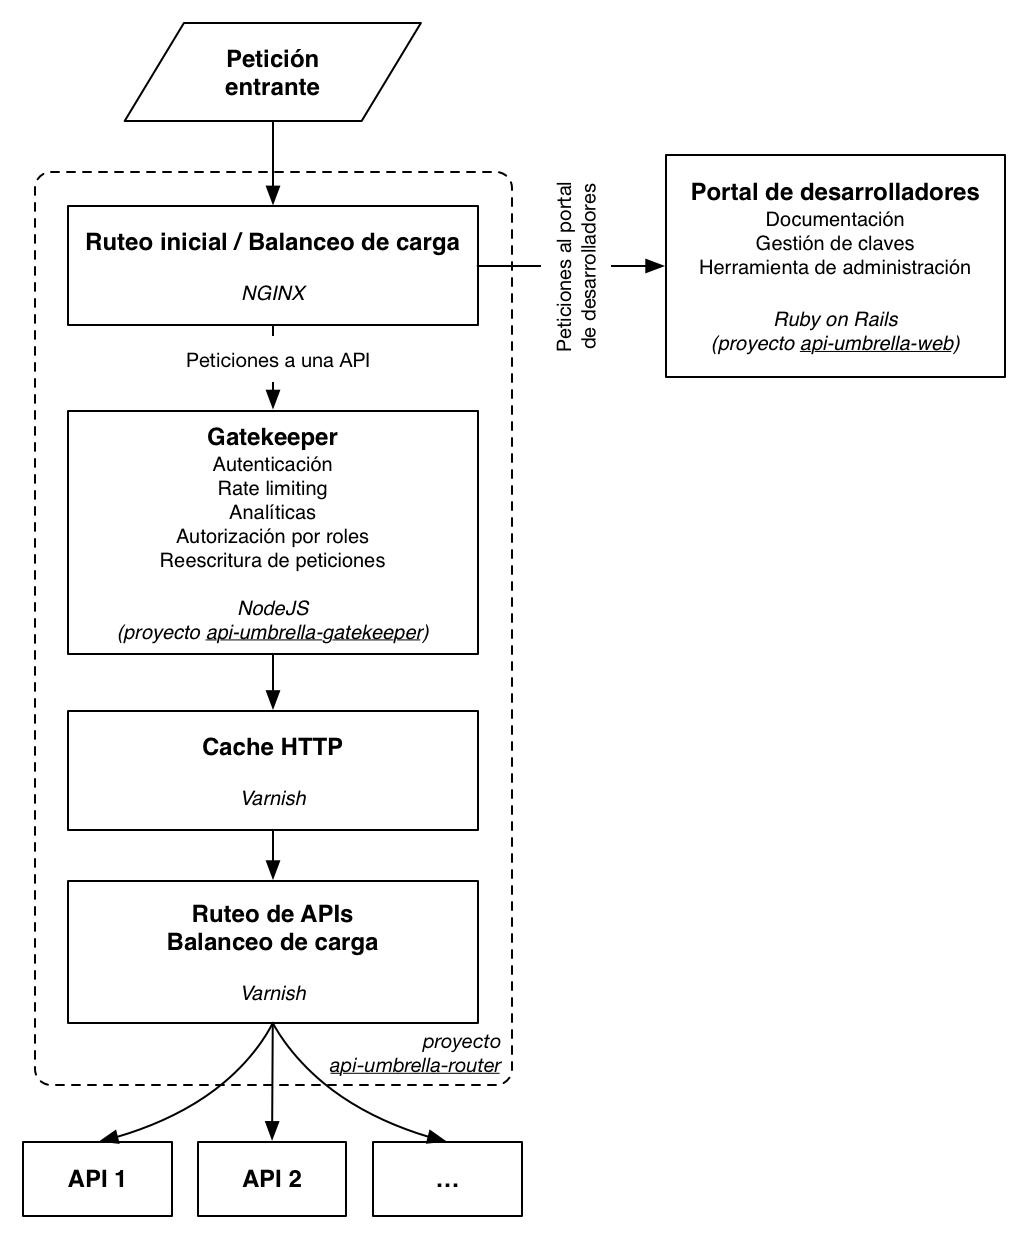
\includegraphics[width=\linewidth]{src/images/03-capitulo-3/tecnologias/api-umbrella/api-umbrella-arquitectura.png}
  \caption{Arquitectura interna de API Umbrella}
  \label{fig:arquitectura-interna-api-umbrella}
\end{figure}

Como se puede ver en la \autoref{fig:arquitectura-interna-api-umbrella}: \nameref{fig:arquitectura-interna-api-umbrella}, según la documentación oficial de la herramienta API Umbrella está compuesto de una serie de elementos que se enlazan secuencialmente, de más externos (cercanos al cliente) a más internos (cercanos a los \eng{backends}):

\begin{itemize}
  \item \textbf{Ruteo inicial con balanceo de carga:} Un servidor \nameref{soa:tecnologias:nginx} recibe las peticiones de los clientes y las deriva al \eng{Gatekeeper} o al sitio para desarrolladores, según sea o no una petición a una \gls{acro:api}.
  \item \textbf{\eng{Gatekeeper}:} Una aplicación hecha en Node.js\footnote{Node.js es un \eng{runtime} para JavaScript basado en V8, el motor de ejecución de ese lenguaje del navegador Google Chrome, que permite ejecutar código escrito en JavaScript del lado del servidor. En la actualidad se encuentra en gran auge por las posibilidades de integración que provee, su velocidad y creciente comunidad de usuarios.\\\url{https://nodejs.org/en/about}} recibe peticiones para las \glspl{acro:api}, aplica restricciones (autenticación, autorización y rate limiting) y transformaciones (reescritura de las peticiones originales), y registra datos de consumo de los servicios para poder utilizarlos con una herramienta de analíticas.
  \item \textbf{Cache HTTP:} Un servidor \nameref{soa:tecnologias:varnish} (Cf. \autoref{soa:tecnologias:varnish}) se ubica justo antes del enrutador de las \glspl{acro:api} para evitar que éstas reciban accesos si la respuesta para el servicio solicitado ya se encuentra en esta cache compartida.
  \item \textbf{Ruteo de servicios con balanceo de carga:} Por último, otro \nameref{soa:tecnologias:nginx} funciona como enrutador de los \glspl{term:endpoint} reales que cada \eng{backend} provee, pudiendo también balancear la carga entre distintas instancias de cada uno.
\end{itemize}

En particular, el \eng{Gatekeeper} merece un gráfico propio describiendo su flujo de trabajo para aplicar restricciones, modificar las peticiones y registrar datos de analíticas. Dicha lógica se puede apreciar en detalle en la \autoref{fig:api-umbrella-gatekeeper}: \nameref{fig:api-umbrella-gatekeeper}. Del detalle del flujo de trabajo de este componente se desprenden el resto de los servicios que completan la arquitectura de API Umbrella:

\begin{itemize}
  \item Bases de datos \gls{db:nosql} MongoDB para almacenar configuración y claves de acceso (\eng{\gls{acro:api} keys}).
  \item Bases de datos clave-valor \gls{db:redis} para almacenar información volátil de los datos de las \glspl{acro:api} y los clientes, como datos del \eng{rate limiting}.
  \item Instancias de Elastic (anteriormente conocido como ElasticSearch), un almacen de datos para búsqueda en texto completo (\eng{full text}) altamente eficiente, donde se almacenan los datos de acceso a los servicios para poder realizar análisis y monitoreo de los mismos.
\end{itemize}

\begin{figure}
  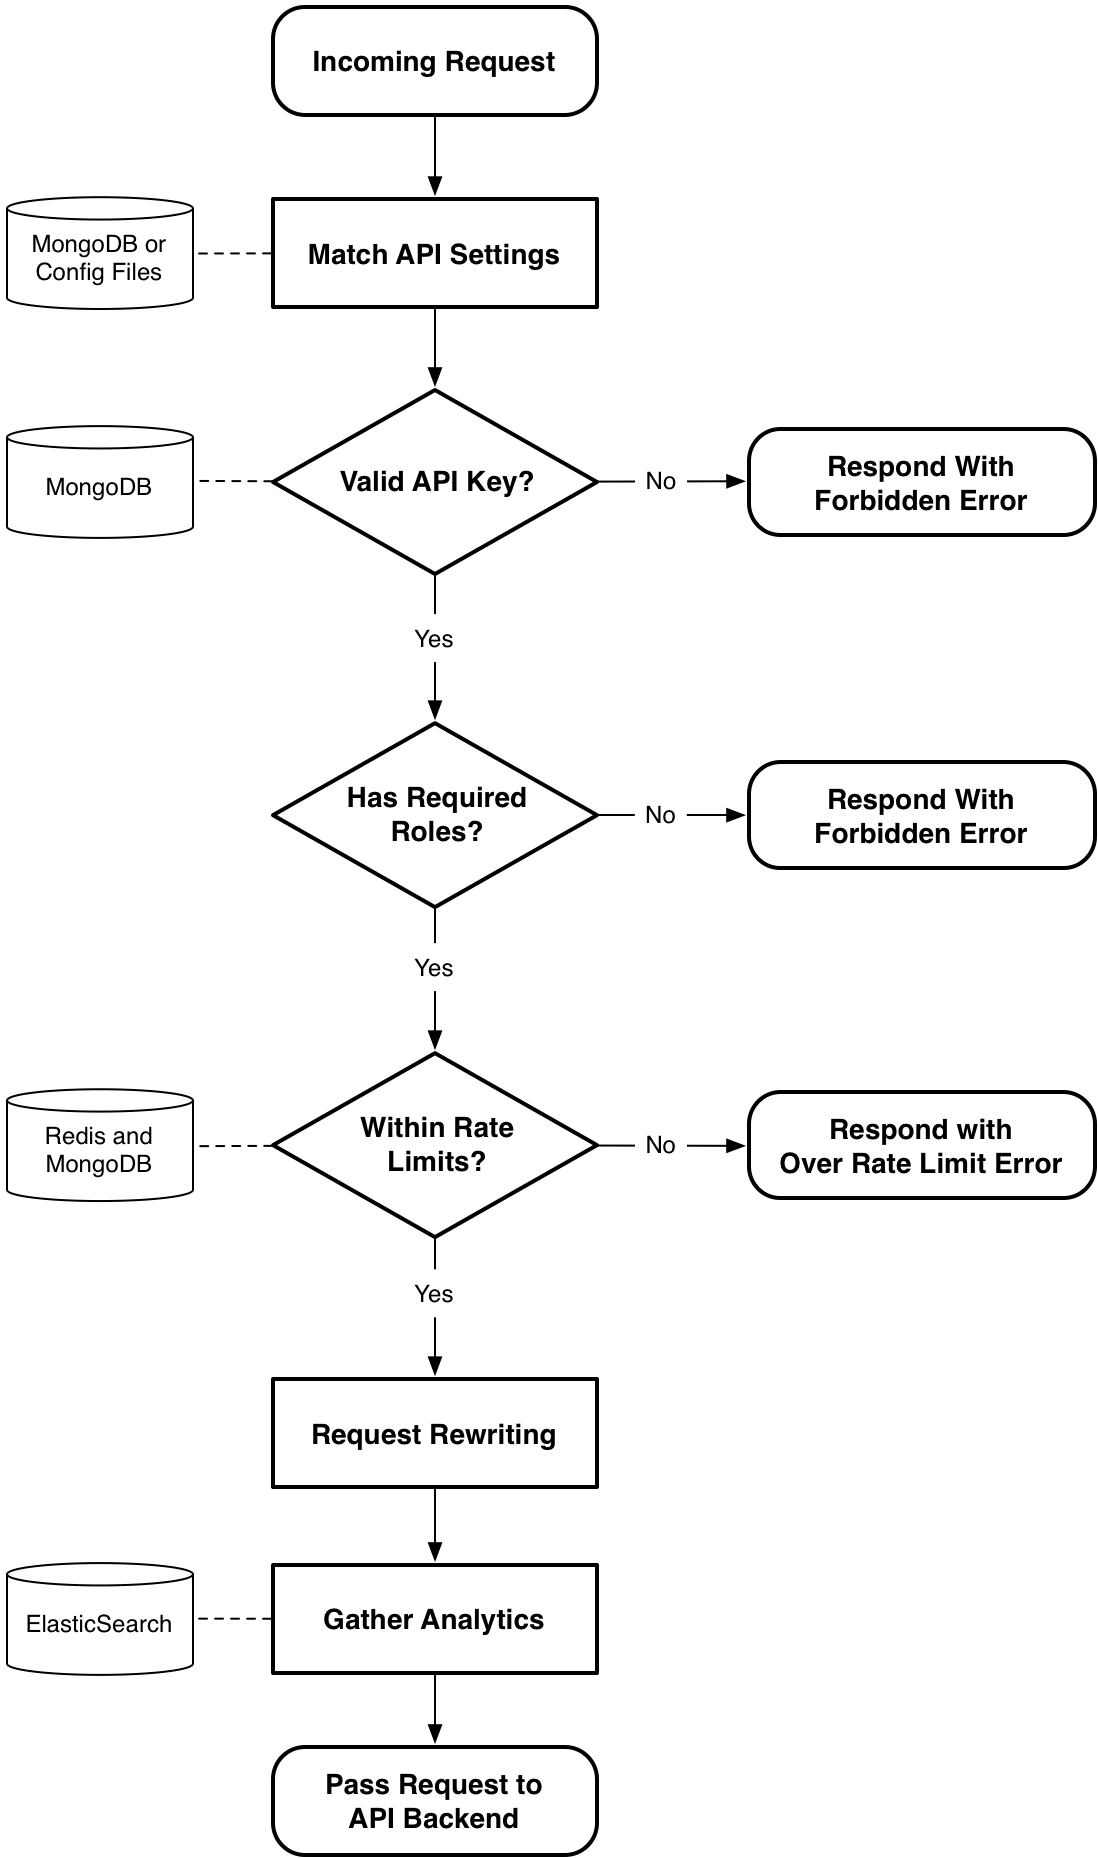
\includegraphics[width=\linewidth]{src/images/03-capitulo-3/tecnologias/api-umbrella/api-umbrella-gatekeeper.png}
  \caption{Lógica de decisión del \eng{Gatekeeper} de API Umbrella}
  \label{fig:api-umbrella-gatekeeper}
\end{figure}

\paragraph{Instalación y prueba}

Al igual que en el caso de \nameref{soa:tecnologias:kong}, y ya que NREL provee una imagen oficial para ejecutar API Umbrella, utilizamos Docker para realizar una prueba de instalación del producto, evaluando sus características, facilidad de instalación y potencial. A continuación detallamos los pasos realizados.

\begin{listing}[H]
  \bashfile{src/03-capitulo-3/tecnologias/nodo-central/code/api-umbrella/00-preparacion.sh}
  \caption{Preparación y arranque de API Umbrella}
  \label{soa:tecnologias:api-umbrella:bash-preparacion}
\end{listing}

Una vez ejecutados los comandos anteriores, tendremos una instancia de API Umbrella en ejecución en el equipo local que podrá ser accedida desde los puertos \texttt{80} y \texttt{443} de \url{localhost}. Adicionalmente al planteo que \nameref{soa:tecnologias:kong} hace con respecto a la forma de administrar el producto mediante el uso de servicios de gestión, API Umbrella también utiliza un archivo de configuración en formato \gls{lang:yaml} que puede resultar más conveniente para poder utilizar un sistema de control de versiones para versionar su contenido, pero que también implica replicarlo en cada instancia del producto que querramos ejecutar.

En el archivo de configuración debemos mínimamente definir las direcciones de correo de los usuarios que podrán acceder a la interfaz web de administración que API Umbrella provee en \url{https://localhost/admin}. Una vez identificados con alguna de esas cuentas de usuario, podremos proceder a utilizar la interfaz web para agregar una \gls{acro:api} para que API Umbrella haga de proxy de la misma. Siguiendo el ejemplo de la documentación del producto, agregamos la \gls{acro:api} de geocodificación de Google, indicando el \eng{\gls{acro:api} backend} con la dirección del servicio provisto por Google y el prefijo de las \glspl{acro:url} que nuestra instancia asociará a dicho servicio (utilizamos \texttt{/google/}), como puede observarse en la \autoref{fig:api-umbrella-api-backend}. Luego de dar de alta esta información, publicamos los cambios mediante la interfaz web y así dejamos públicamente disponible el servicio de geocodificación en nuestra instancia de API Umbrella mediante el prefijo de \gls{acro:url} \url{http://localhost/google/}.

\begin{figure}
  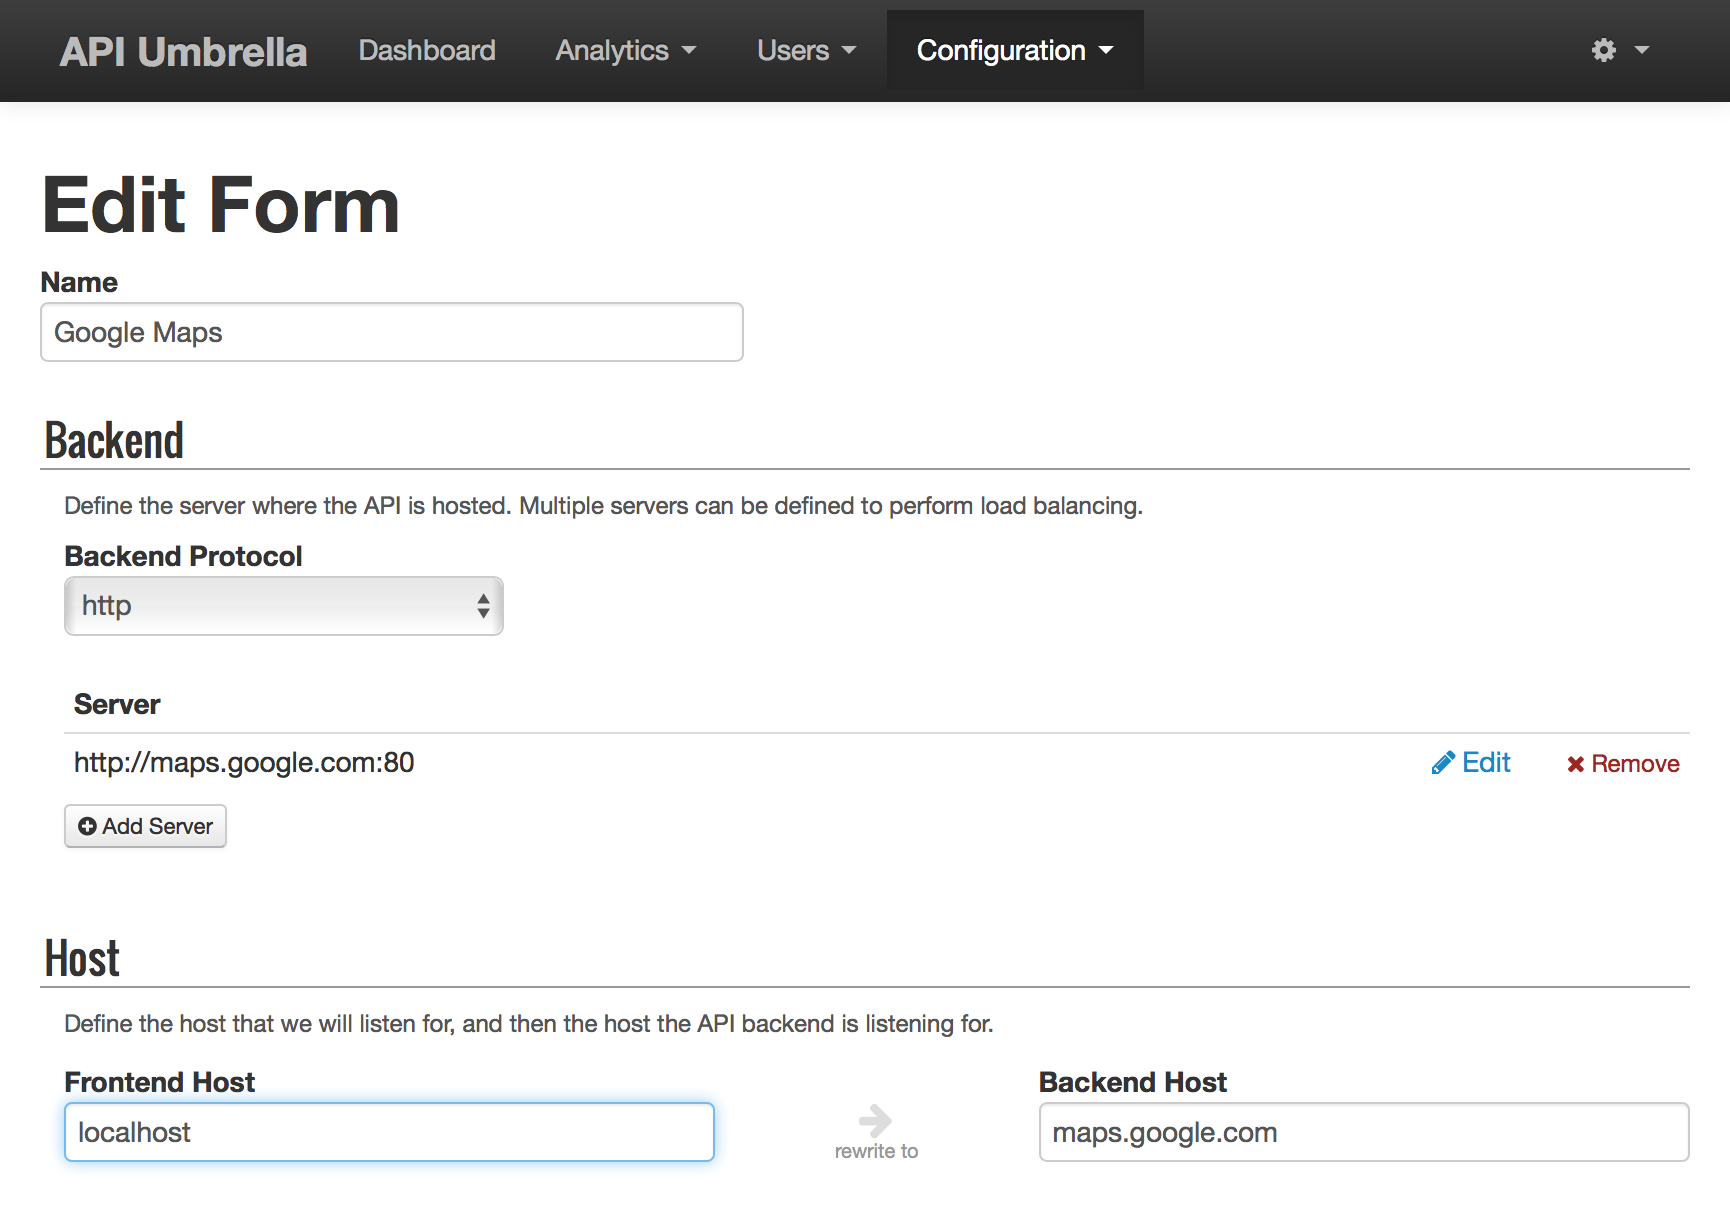
\includegraphics[width=\linewidth]{src/images/03-capitulo-3/tecnologias/api-umbrella/api-backend.png}
  \caption{Interfaz web de carga de un \eng{backend} de servicios de API Umbrella}
  \label{fig:api-umbrella-api-backend}
\end{figure}

Para poder utilizar este nuevo \gls{term:endpoint} es necesaria una clave de acceso (\eng{\gls{acro:api} key}), para lo cual API Umbrella provee una interfaz web dedicada. Completando los datos solicitados obtendremos nuestra clave de acceso para que nuestras peticiones sean autorizadas (en nuestro caso obtuvimos la clave \texttt{6dn6iL7xTuR1bvSWdRccpP7DCFp5X2OnhdYZzkrI}). Utilizando esta clave y la \gls{acro:url} definida anteriormente, podemos realizar las peticiones detalladas en el bloque de código \autoref{soa:tecnologias:api-umbrella:bash-pruebas} para probar el correcto funcionamiento del producto, haciendo una petición sin credenciales primero y luego la misma petición incluyendo la información de autenticación. Al hacer esto, intentamos corroborar que la primer petición sea denegada mientras que la segunda obtenga la respuesta exitosa esperada.

\begin{listing}[H]
  \bashfile{src/03-capitulo-3/tecnologias/nodo-central/code/api-umbrella/01-pruebas.sh}
  \caption{Prueba de uso de API Umbrella}
  \label{soa:tecnologias:api-umbrella:bash-pruebas}
\end{listing}

Con estas pruebas pudimos comprobar varias situaciones:

\begin{itemize}
  \item En primer lugar, que API Umbrella requiere por defecto el uso de claves de acceso para responder a los servicios para los que funciona de proxy. Este enfoque ``seguro por defecto'' es altamente deseable, ya que implica que para consumir la información que nuestros servicios proveen, se debe obtener una clave de acceso y por ende se debe identificar al cliente (\eng{consumer}) de la información - en nuestro caso, serían las aplicaciones cliente las que identifiquemos, pero si llegásemos a proveer nuestra información a terceros, éstos deberían primero identificarse para obtener una clave de acceso y así permitirnos tener una noción de quién y cuánto utiliza nuestra información.
  \item En segundo lugar, que efectivamente hay un \nameref{soa:tecnologias:varnish} funcionando internamente a API Umbrella. Esto se hace evidente en las cabeceras que esta cache compartida agrega a las respuestas \gls{proto:http}: \texttt{X-Cache} y \texttt{Age}. Adicionalmente, API Umbrella agrega las cabeceras correspondientes para indicar cuándo y por cuánto tiempo se pueden almacenar en caches intermedias las respuestas, mediante \texttt{Cache-Control} y \texttt{Expires}.
  \item También comprobamos que las respuestas tienen límites en la tasa de consultas que podemos hacer. Esto se hace evidente en las cabeceras \texttt{X-RateLimit-Limit} y \texttt{X-RateLimit-Remaining} que indican respectivamente el límite aplicable y la cantidad de peticiones que nos quedan disponibles hasta que se cumpla el período de tiempo del límite y esos contadores se reinicien.
  \item Y por último, aunque no por eso menos importante, que el producto funciona correctamente haciendo de proxy del servicio de geocodificación de Google, al devolvernos una respuesta correcta para nuestra consulta.
\end{itemize}

Luego de realizar algunas peticiones, podemos utilizar la potente herramienta de análisis de tráfico y respuestas que provee API Umbrella para tener una idea del uso que nuestra instancia está teniendo, junto con datos como quién, cuándo, cuánto, cómo y desde dónde está usando nuestras \glspl{acro:api}. En la \autoref{fig:api-umbrella-analytics} se puede apreciar, a modo de ejemplo, parte de la información que se puede obtener mediante esta herramienta.

\begin{figure}
  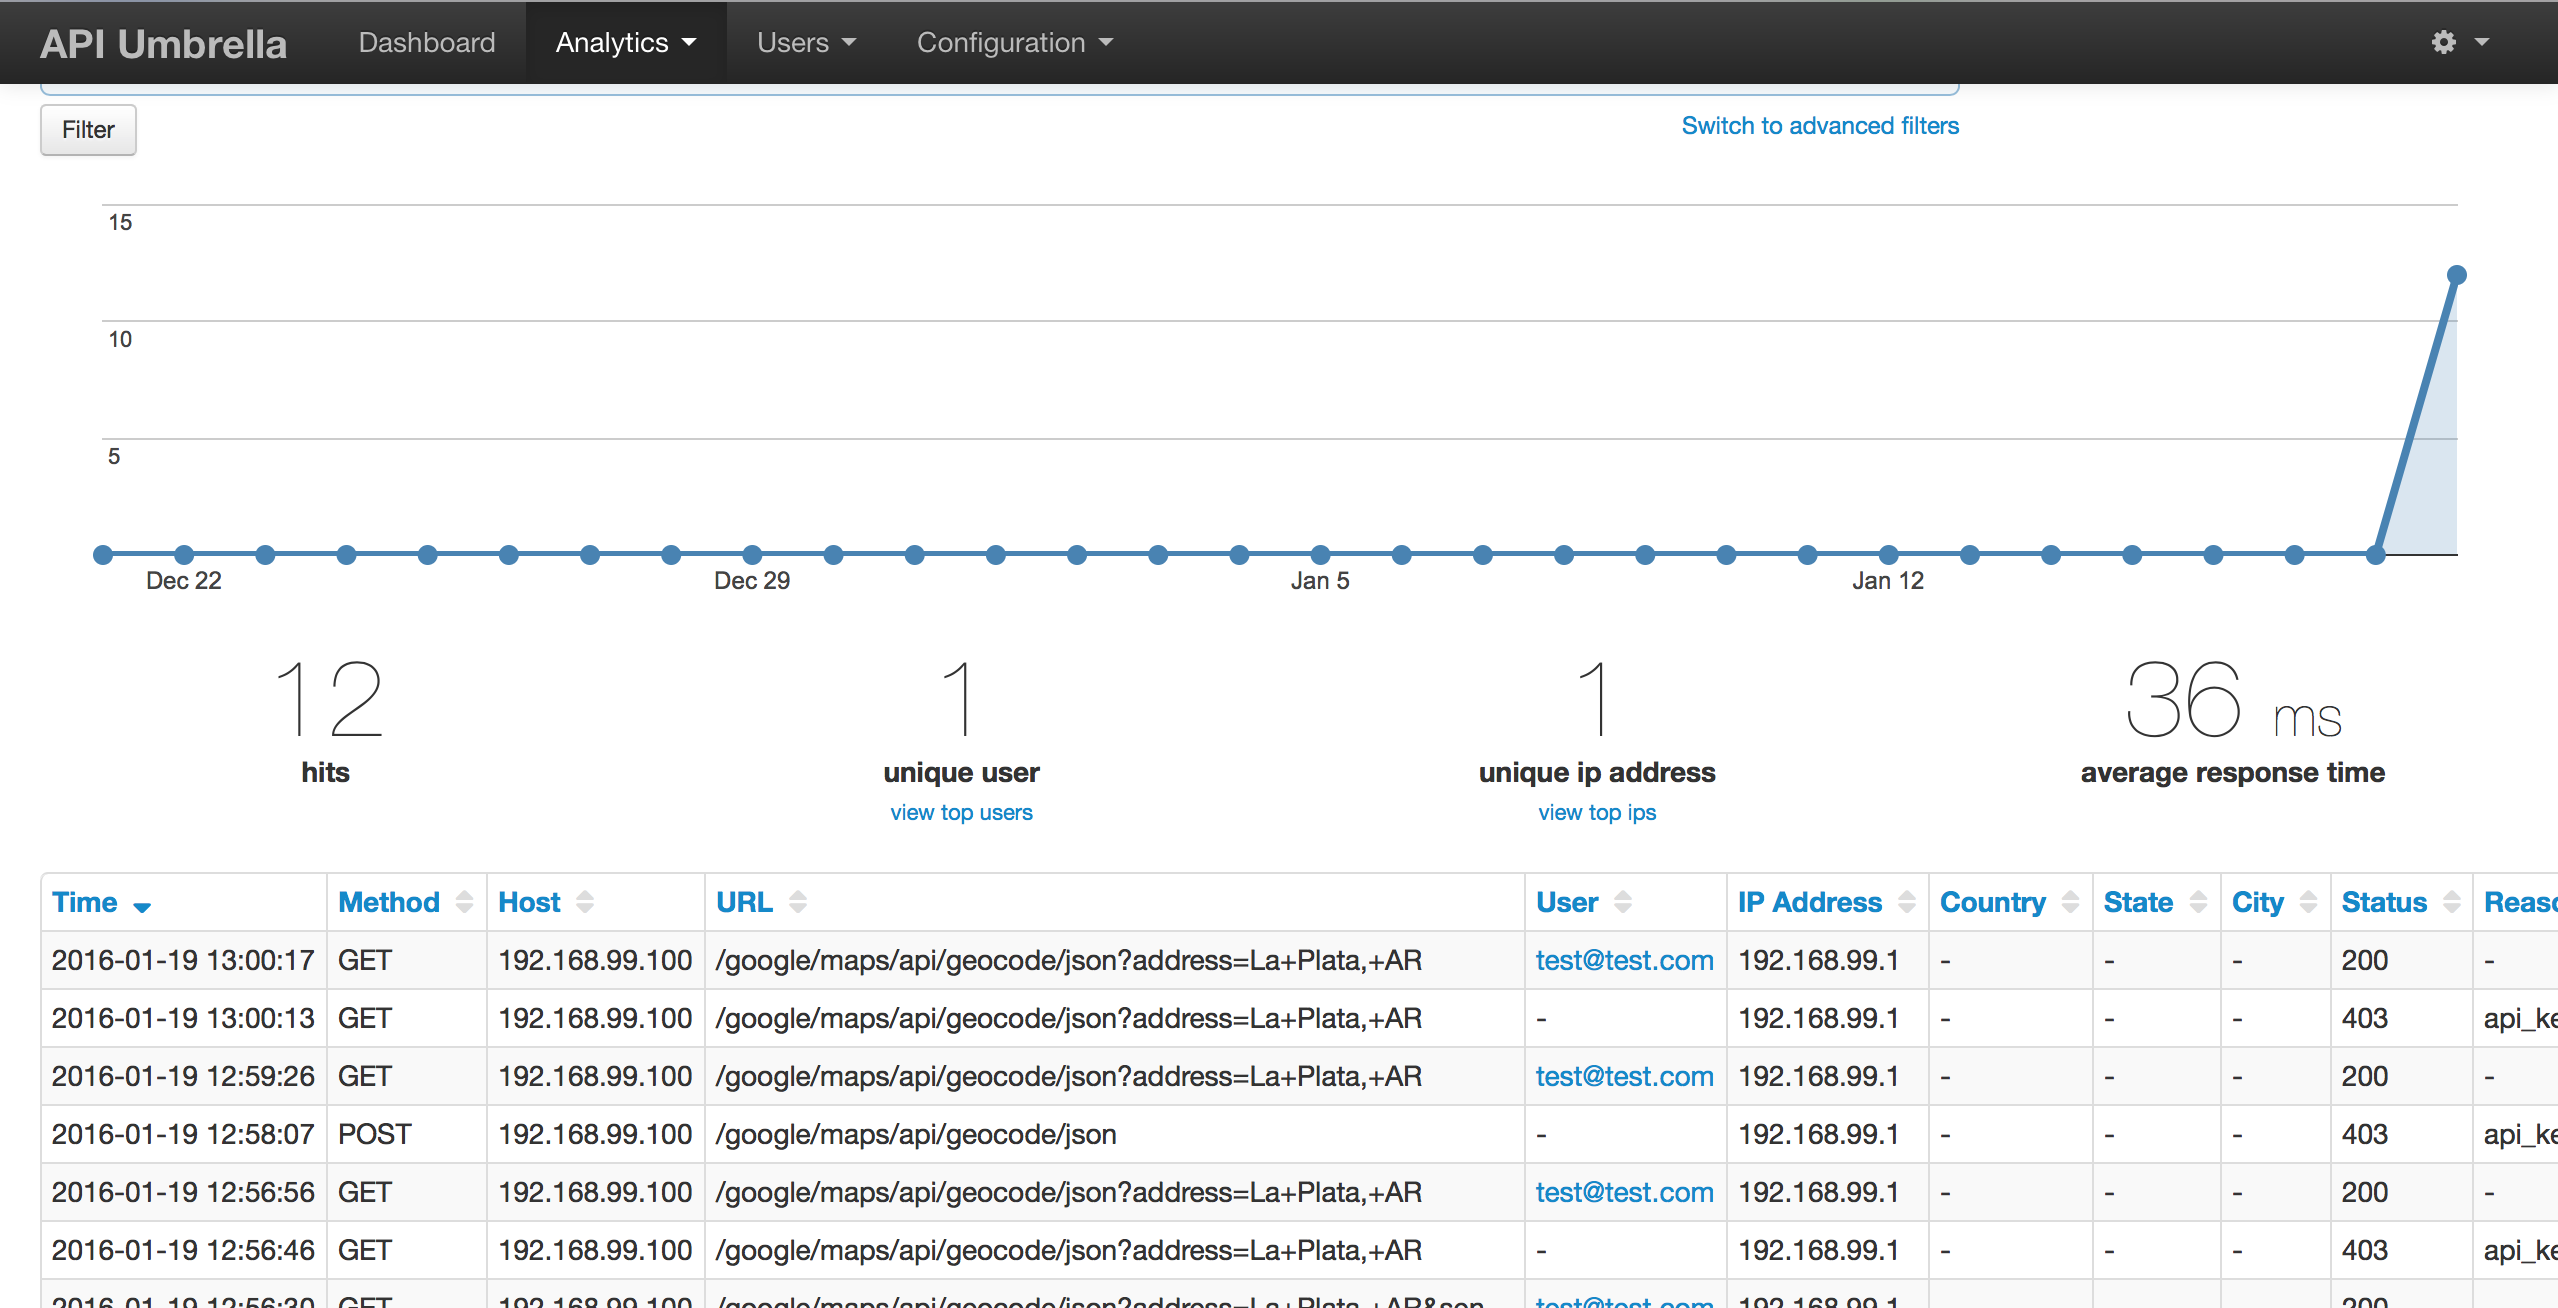
\includegraphics[width=\linewidth]{src/images/03-capitulo-3/tecnologias/api-umbrella/analytics.png}
  \caption{Interfaz web de análisis del uso de los servicios de API Umbrella}
  \label{fig:api-umbrella-analytics}
\end{figure}

\paragraph{Madurez}

Al momento de comenzar a analizar los productos para el presente trabajo, API Umbrella se encontraba en activo desarrollo, definición y evolución. Su arquitectura interna era muy cambiante y aún le faltaban pruebas reales en ambientes productivos para poder cerrar las definiciones, por lo cual sus propios autores aconsejaban su uso únicamente para desarrollo\footnote{Hasta Diciembre de 2015, la documentación oficial del producto mostraba la leyenda ``\eng{This version is for development only}'' (``Esta versión es únicamente para desarrollo'')}.

Con la llegada de 2016 su desarrollo se desaceleró y la arquitectura quedó estabilizada, pero al momento de escritura del presente informe la herramienta carece de pruebas en producción que respalden las características que la documentación oficial describe y que nos den confianza que el producto se encuentre realmente maduro.

\subsubsection{API Axle}
\label{soa:tecnologias:api-axle}

Este es otro producto que comenzamos a analizar ya que parece tener características similares a \nameref{soa:tecnologias:kong} y \nameref{soa:tecnologias:api-umbrella}:

\begin{itemize}
  \item Funciona como un proxy reverso que se ubica delante de los servicios que queremos que provea.
  \item Utiliza \nameref{soa:tecnologias:nginx} como base para atender requerimientos entrantes.
  \item Implementa limitación de tasa de consultas, autenticación por clave de acceso, cache de respuestas, entre otros.
  \item Almacena en una base de datos \gls{db:redis} las estadísticas de uso.
\end{itemize}

\paragraph{Licencia}

Este producto está licenciado bajo GPL v3\footnote{\url{https://github.com/apiaxle/apiaxle/blob/develop/GPL-3.0.txt}}.

\paragraph{Estado del proyecto}

Lamentablemente, al indagar un poco más en profundidad sobre este producto notamos que el proyecto no tiene actividad desde mayo de 2015 y que su documentación es escasa e incompleta. La falta de ejemplos reales y de casos testigo que respalden el uso de la herramienta completan un panorama no muy alentador para considerar esta herramienta entre las opciones para nuestra nueva arquitectura.

\subsubsection{Tyk}
\label{soa:tecnologias:tyk}

Tyk es un API Gateway liviano y plataforma de administración, todo en un mismo producto, que permite controlar quien tiene acceso a la API, cuando y como.  Escrito en Go, sencillo de configurar, sus únicas dependencias son Redis y MongoDB (v2.6 o superior, requerido para el almacenamiento de los datos de acceso, opcional)

El API Gateway de Tyk se implementa delante de nuestras \glspl{acro:api} para gestionar la autorización, control de acceso y limitación de acceso (\eng{rate limiting}) a nuetros servicios.  De esta manera permite concentranos en el desarrollo de servicios para nuestras \glspl{acro:api}, en lugar de implementar herramientas para la administración de la infraestrucutra, simplemente se desarrollo el servicio, el cual puede ser integrado fácilmente al API Gateway.

Tyk posee un portal para desarrolladores que permite analizar quien y como utilizan nuestras \glspl{acro:api}, limitar el acceso a los servicios (\eng{rate limiting}), utlización de \eng{caching}, generar o rebocar una \eng{Key}, entro otras características.  Todo esto de manera muy sencilla y centralizada, evitando trasladar parte de esta funcionalidad a las \glspl{acro:api}.

\paragraph{Licencia}

Tyk se encuentra publicado bajo licencia Mozilla Public License Version 2.0\footnote{La misma puede ser consultada accediendo a \url{https://www.mozilla.org/en-US/MPL/2.0}}.

\paragraph{Características principales}

A continuación presentamos un breve listado de las características principales que Tyk ofrece actualmente:

\begin{itemize}
  \item RESTful API - posee una \gls{acro:api} RESTful, que permite configurar Tyk.
  \item Multiple access protocols - Tyk soporta múltiples métodos de acceso a la \gls{acro:api}: \eng{Token-based}, \eng{HMAC}, \eng{Basic Auth}, \eng{OAuth2}, \eng{JSON Web Token} y \eng{Keyless}. \\
  \url{https://tyk.io/v1.9/access-control/keyless} \\
  \url{https://tyk.io/v1.9/access-control/json-web-tokens} \\
  \url{https://tyk.io/v1.9/access-control/basic-auth} \\
  \url{https://tyk.io/v1.9/access-control/hmac} \\
  \item Rate Limiting - permite configurar fácilmente el \eng{rate limit} para cada \eng{API Key}, definiendo la cantidad de peticiones por segundo y el tiempo de expiración (1 hora, 6 horas, 12 horas, 24 horas, 1 semana, 1 mes o nunca expira). \\
  \url{https://tyk.io/v1.9/quotas-limits-security/access-control}
  \item Policies - permite crear políticas para aplicar \eng{quotas}, \eng{rate limit} y \eng{access rights} a un conjunto de \eng{Keys}. \\
  \url{https://tyk.io/v1.9/quotas-limits-security/limiting-access}
  \item Path by path permissions - permite configurar permisos de acceso para cada \eng{endpoint}, indicando el método.
  \item Key Expiry - permite controlar el tiempo de expiración de una \eng{Key}. \\
  \url{https://tyk.io/v1.9/rest-api/api-key-management}
  \item API Versioning - permite versionar la API de tres maneras diferentes:
  \begin{itemize}
    \item mediante una clave en el encabezado http, por ej. x-api-version
    \item por URL o parámetro en el Form
    \item por el primer elemento de una URL, ej. /v1/resource/id
  \end{itemize}
  \url{https://tyk.io/v1.9/api-management/api-versioning}
  \item Analyitcs logging - registro detallado de los accesos a las \glspl{acro:api}.
  \item Zero downtime restarts - las configuraciones de Tyk pueden realizarse dinámicamente, reiniciar los servicios sin que esto afecte los requerimientos activos.
  \item Web hooks - fácilmente se pueden integrar notificaciones y eventos que permitirán mejorar el monitoreo.
  \item IP White-listing - acceso autorizado solo a las direcciones IP indicadas
  \item Size Limits - permite limitar el tamañan de las peticiones que llegan a las \gls{acro:api}, evitando que los sevicios sean saturados por peticiones.
  \item Health checks - permite verificar el estado de los nodos.
  \item Mock APIs - permite crear \glspl{acro:api} de prueba.
  \item API Blueprint support - permite importar rápidamente una \gls{acro:api} en formato JSON.
  \item Swagger support - permite importar archivos que respeten \nameref{soa:tecnologias:openapi-spec} (anteriormente conocida como \eng{The Swagger specification}).
  \item Request and Response transformations - permite utilizar templates para transformar datos y agregar o quitar header \eng{on-the-fly}
  \item Caching - permite implementar una cache para las respuestas por \eng{endpoint} o globalmente, incrementando la velocidad de respuesta, al mismo tiempo que se disminuye la carga de las \gls{acro:api}. \\
  \url{https://tyk.io/v1.9/api-management/caching}
  \item API Documentation, el portal de Tyk soporta API Blueprint y Swagger.
  \item Virtual Endpoints, como AWS Lambda functions, permite correr fragmentos de JavaScript en los \eng{endpoints} para manejar interacciones complejas de servicios, tales como solicitud de procesamiento por lotes. \\
  \url{https://tyk.io/v1.9/api-management/virtual-endpoints}
  \item Focus on microservices, permite implementar el patrón \eng{circuit breaker}, hard timeouts y \eng{round-robin}, para balancear la carga en el acceso a los servicios. \\
  \url{https://tyk.io/v1.9/api-management/circuit-breakers} \\
  \url{https://tyk.io/v1.9/api-management/load-balancing}
  \item Uptime Awareness, Tyk activamente monitorea los \eng{endpoints} de las \glspl{acro:api} y notifica cuando alguno de estos se encuentra fuera de servicio. \\
  \url{https://tyk.io/v1.9/uptime-tests/uptime-tests}
\end{itemize}

\paragraph{Instalación y prueba}

A continuación se detallan los pasos necesarios para la instalación y ejecución de Tyk, basándonos en su documentación oficial \footnote{\url{https://tyk.io}}.

Tyk puede instalarse de varias maneras:

\begin{itemize}
  \item Instalación de Tyk en Ubuntu desde paquetes
  \item Instalación de Tyk en Redhat o CentOS usando paquetes RPM
  \item Instalación de Tyk desde una imagen Docker
\end{itemize}

En nuestro caso particular se optó por instalar Tyk en Ubuntu 14.04 desde paquetes, por lo tanto a continuación desarrollaremos esta forma de instalación.

Pre-requisites:

Asegurarse que el puerto 8080 esté abierto: este puerto es utlizado por el API Gateway
Asegurarse que el puerto 3000 esté abierto: este puerto es utlizado por el dashboard, quien provee la GUI y el portal para desarrolladores

Para iniciar los dos servicios requeridos por Kong para su funcionamiento (Apache Cassandra y Kong mismo), ejecutamos la siguiente secuencia de comandos:

\begin{listing}[H]
  \bashfile{src/03-capitulo-3/tecnologias/nodo-central/code/tyk/00-preparacion.sh}
  \caption{Preparación y arranque de Tyk}
  \label{soa:tecnologias:tyk:bash-preparacion}
\end{listing}


\paragraph{Integración con nuestro diseño}

\begin{figure}[H]
  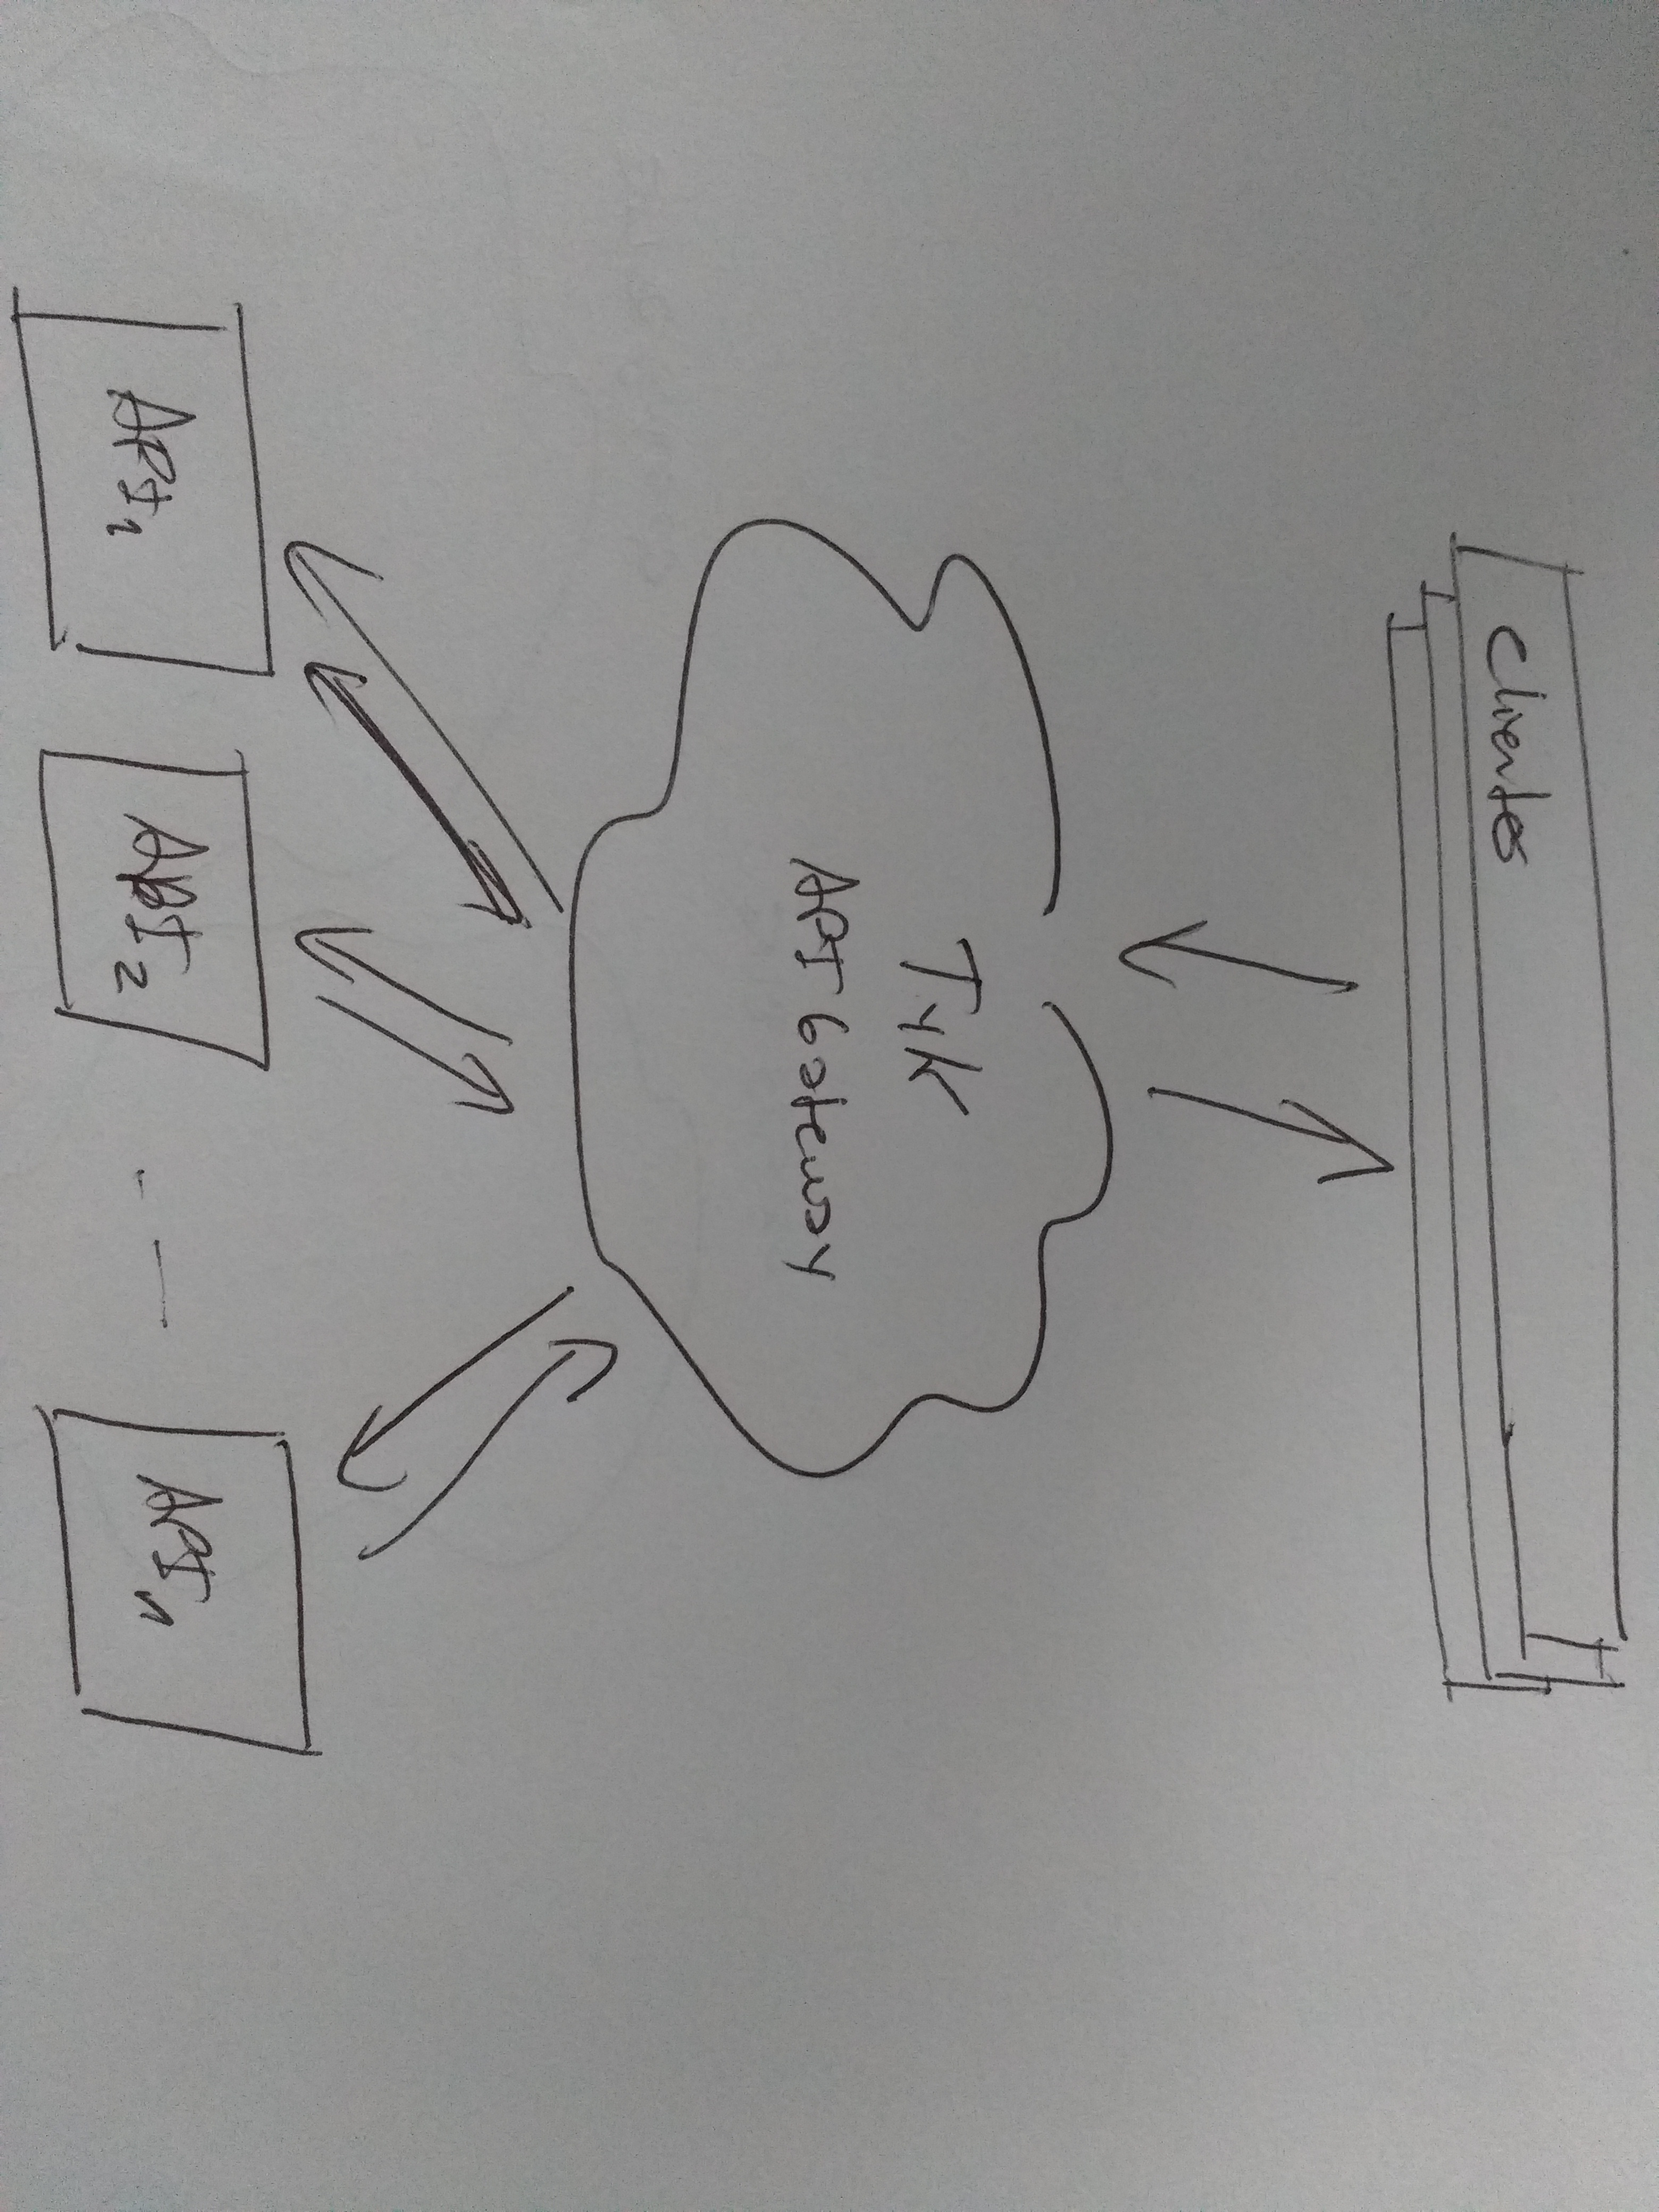
\includegraphics[width=\linewidth]{src/images/03-capitulo-3/tecnologias/tyk/tyk-arq.jpg}
  \caption{Esquema de integración de Tyk en nuestra propuesta}
  \label{fig:integracion-tyk-arquitectura}
\end{figure}

Para el nuevo diseño de la arquitectura, se implementaría la API Gateway de Tyk como un nodo central, por donde se enrutarían todas las peticiones realizadas desde los diferentes clientes.  Detrás de Tyk tendremos replicadas N instancias de las \glspl{acro:api}, las cuales nos permiten escalar horizontalmente de forma sencilla, Tyk se encargará de realizar el balanceo de la carga a cualquiera de estas instancias replicadas.

La migración de la vieja nube a la nueva arquitectura, se iría realizando de manera progresiva, cambiando el viejo cliente por el nuevo, en cada aplicación.  De esta manera tendremos conviviendo al mismo tiempo, la vieja nube y la nueva arquitectura.

\paragraph{Conclusión}

Kong o Tyk, porque...

\textit{TODO: Acomodar las conclusiones que estaban en los productos para unificarlas comparativamente:}

\subparagraph{Conclusión (tomada de API Axle)}

La falta de mantenimiento, documentación y datos que respalden la posibilidad de usar API Axle seriamente en producción, sumados a la complejidad para instalar la herramienta para hacer una prueba de concepto nos detuvo al momento de continuar analizando este producto.

\subparagraph{Conclusión (tomada de API Umbrella)}

API Umbrella se ve muy prometedor, es un producto más grande que otros que hemos analizado como \nameref{soa:tecnologias:kong}, lo cual da soporte para algunas características que no están presentes en el resto como el uso de \nameref{soa:tecnologias:varnish} como cache compartida dentro del mismo proxy, pero presenta un gran inconveniente para considerarlo como una opción en nuestra arquitectura: su nivel de madurez. En el diseño final para la nube de servicios necesitamos utilizar herramientas estables, listas para ser utilizadas en servicios en producción y API Umbrella aún no puede ser considerada lo suficientemente madura y probada como para ser una candidata fuerte para ser incluida en nuestra arquitectura.

\subparagraph{Conclusión (tomada de Kong)}

Kong es una excelente alternativa al uso de un \gls{acro:esb}, ya que es más liviano, sencillo de configurar y administrar, altamente extensible y personalizable, y cubre las necesidades que tenemos en cuanto a escalabilidad, transparencia, centralización de la gestión y portabilidad.


\subsection{Para balancear la carga}
\label{soa:tecnologias:para-balancear}

\subsubsection{Apache}
\label{soa:tecnologias:apache}

Ver \url{http://httpd.apache.org/docs/2.2/mod/mod_proxy_balancer.html}

\paragraph{NGINX}
\label{soa:tecnologias:nginx}

\subsubsection{Conclusión}

A partir del análisis realizado y de nuestra propia experiencia, en la que hemos utilizado ambos servidores, consideramos que \nameref{soa:tecnologias:nginx} es la mejor opción dadas las expectativas de crecimiento que tenemos para este nodo de la nube de servicios.

Su esquema de alta disponibilidad, con bajo consumo de recursos, poco mantenimiento requerido y su activa comunidad son factores determinantes en nuestra decisión.


\subsection{Para documentar}
\label{soa:tecnologias:para-documentar}

Como desarrolladores conocemos la importancia de una buena documentación, que se encuentre actualizada y pensada en ayudar, que invite a utilizarla y que sea fácil de consultar. En la actualidad, la nube de servicios carece de una documentación que cumpla con estos requisitos, lo cual produce situaciones poco deseables para quienes utilizamos sus servicios, ya que esto, sumado a la falta de consistencia en las respuestas y los parámetros admitidos, hacen que debamos consultar el código fuente con demasiada frecuencia.

En este apartado analizaremos herramientas que proponen estándares de documentación para \glspl{acro:api} e intentan asistir a mantener utilizable y al día la información de consulta sobre los servicios que éstas ofrecen.

\subsubsection{API Blueprint}
\label{soa:tecnologias:api-blueprint}

Ver \url{https://apiblueprint.org/}

\subsubsection{RAML}
\label{soa:tecnologias:raml}

Entre las alternativas sobresalientes para la documentación de \glspl{acro:api} \gls{acro:rest}, encontramos en RAML un conjunto extenso de funcionalidades que no se limita únicamente a la generación de una \gls{term:documentacion-viviente} para nuestros servicios, si no que además permite generar código y tests para realizar pruebas a unidad sobre nuestros \glspl{term:endpoint} mediante el uso de herramientas complementarias diseñadas para esta tecnología.

RAML, cuyo nombre es el acrónimo para \eng{RESTful API Modeling Language}, es una especificación y un lenguaje de descripción de \glspl{acro:api} \gls{acro:rest} basado en \gls{lang:yaml}, diseñado por un grupo de trabajo integrado por importantes empresas de la industria como Cisco, VMWare, Mulesoft e Intuit. Su premisa es ser una especificación abierta, sin ser dirigida a un proveedor específico, y que su estructura permita describir \glspl{acro:api} \gls{acro:rest} de manera clara, correcta, precisa, consistente, legible, natural e intuitiva.

\paragraph{Licencia}

RAML se encuentra liberado bajo la licencia Apache versión 2.0\footnote{\url{http://raml.org/about/legal}}.

\paragraph{Estructura}

Al escribir la descripción de una \gls{acro:api} \gls{acro:rest} con RAML, debemos crear un archivo principal con extensión \texttt{.raml} que contendrá el nodo raiz de la especificación de los servicios. En ese nodo se define la versión de RAML a utilizar\footnote{Al momento de escritura del presente informe, la versión más reciente de RAML es la \texttt{1.0}}, el título que le damos a la \gls{acro:api}, su dirección base y algunos atributos opcionales como por ejemplo la versión.

Adicionalmente, se definen los recursos que los servicios pueden proveer, identificándolos por sus \glspl{acro:uri}, y anidándolos en caso que se trate de recursos que tengan esa organización. Bajo estas claves que indican los servicios (o sus \glspl{acro:uri}, más precisamente) se especifican qué métodos \gls{proto:http} admite cada \gls{acro:uri}, junto con un detalle de los parámetros que admita (en caso que aplique). Además de describir los servicios y la forma de realizar las peticiones, RAML permite describir las respuestas mediante el uso de ejemplos o esquemas genéricos, agrupándolos por código de estado \gls{proto:http}.

Al ver la forma en que se estructuran las especificaciones RAML, rápidamente notamos que es un formato orientado a la reutilización de recursos y definiciones, buscando en todo momento evitar la repetición innecesaria de información, lo cual es una consideración positiva a la hora de planificar una especificación donde es altamente probable que tanto datos como esquemas se repitan en distintos puntos. En el mismo sentido, permite incluir en cualquier punto de un archivo \texttt{.raml} el contenido de otro archivo para utilizar su contenido, sin que necesariamente se trate de otro archivo con el mismo formato. Esto también asiste a la simplificación del trabajo de documentación y la reutilización de los recursos definidos a lo largo de la especificación que se realiza.

\paragraph{Herramientas}

El ecosistema de herramientas alrededor de RAML es variado, con implementaciones de su \eng{Parser} en los lenguajes más populares, y con algunas librerías (principalmente implementadas en JavaScript mediante Node.js) para servir la \gls{term:documentacion-viviente} generada a partir de los documentos RAML, y con otras para generar tests automatizados de las \glspl{acro:api} \gls{acro:rest} descriptas mediante este lenguaje. Este último punto es una gran ventaja, considerando la importancia que tienen las pruebas automatizadas sobre los servicios críticos que provee la nube de servicios de la UNLP.

\paragraph{Swagger}
\label{soa:tecnologias:swagger}

Ver \url{http://swagger.io/}

\subsubsection{Conclusión}

¿Swagger?, porque...



\newpage

  %   - Capítulo IV
  \section{Capítulo IV: Propuesta de rediseño}
\label{cap4}

\todo{Escribir una breve introducción para este capítulo}

\textit{En este capítulo se documentan el caso testigo y el desarrollo del prototipo para ejemplificar. A partir de esto se debe desprender una conclusión. Posiblemente se enumeren acá los trabajos a futuro, principalmente la implementación efectiva del diseño que aquí planteamos.}

\subsection{Propuesta de diseño}
\label{propuesta}

\todo{Relacionar REST con nuestra propuesta. Utilizar como referencia el capítulo 6 de Fielding: \url{https://www.ics.uci.edu/~fielding/pubs/dissertation/evaluation.htm} y tomar la \autoref{fig:ejemplo-rest-nueva-arquitectura}}

\begin{figure}
  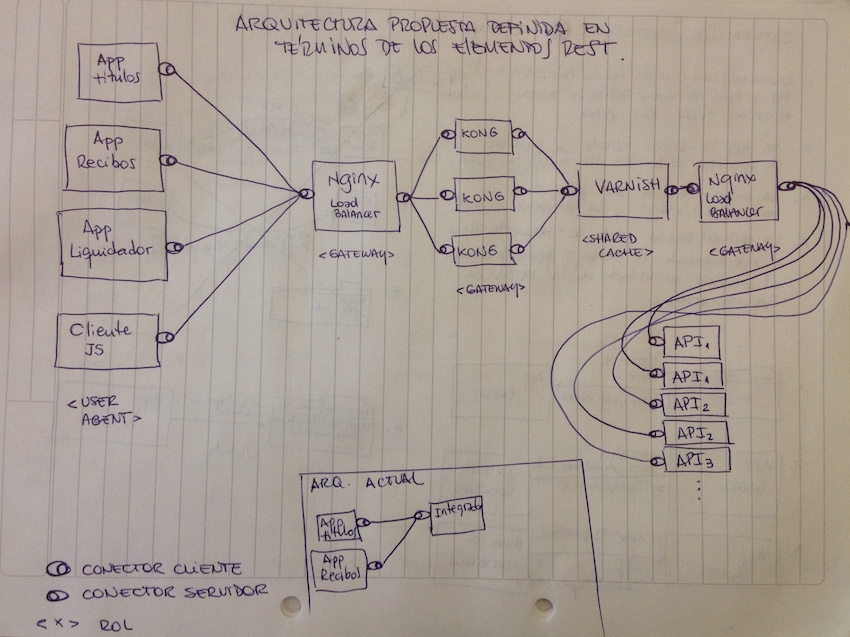
\includegraphics[width=\linewidth]{src/images/04-capitulo-4/nueva-arq-segun-rest.jpg}
  \caption{Visión \gls{acro:rest} de la nueva arquitectura propuesta}
  \label{fig:ejemplo-rest-nueva-arquitectura}
\end{figure}

\todo{Decir que se van a implementar como microservicios, aprovechando lo detallado en la \autoref{microservicios}.}

% ver en http://www.oreilly.com/programming/free/open-by-design.csp?download=yes&order=574386
% se puede sacar algo referente al opensource
% otro que puede servir Migrating to the Cloud?

Por lo expuesto anteriormente, se propone una arquitectura más desacoplada a la planteada con el Integrador, permitiendo de esta manera minimizar el costo del mantenimiento, desarrollo y simplificando su instalación (\eng{deployment}) en entornos de producción. Una solución basada en estándares que permita integrar sistemas heterogéneos, aceptando el hecho de que la mayoría de los sistemas legados que se encuentran en producción, se mantendrán y logrando de esta manera, que la infraestructura subyacente facilite la incorporación de cambios que puedan surgir como necesidades del \cespi y la \unlp.

El modelo de servicios facilita el acceso y consumo de la información a través de la red. Dado que los servicios son independientes y autónomos, pueden combinarse tantas veces como sea necesario de manera sencilla, generando nuevas aplicaciones que respondan a las necesidades en constante evolución de nuestra Casa de estudios. Esta posible agregación y combinación de servicios para resolver situaciones presentes y futuras convierten en una opción altamente beneficiosa el uso de una estrategia orientada a servicios, con el fin de crear servicios y aplicaciones compuestas que pueden existir con independencia de las tecnologías subyacentes\cite{microsoft2006}.

El resultado final es una nube, con conjunto de servicios y una creciente flota de aplicaciones dependientes de éstos, que se adapta fácilmente a los cambios.

En este capítulo profundizaremos la aplicación concreta de los conceptos vistos hasta aquí en el presente trabajo, explicando a través de los puntos mencionados en la \autoref{objetivo}.


\subsubsection{Redundancia y escalabilidad}

Cuando hablamos de escalabilidad, podemos basarnos en el modelo llamado \eng{scale cube}\cite{website:akfpartners-scale-cube}. Este modelo clasifica las distintas formas de escalar las aplicaciones en 3 sentidos, tomando como analogía las 3 dimensiones de un cubo:

\begin{itemize}
  \item \textbf{Escalar sobre el eje \textit{X}:} (\eng{X-axis scaling}, en inglés) Esta es la técnica más comúnmente utilizada para incrementar la disponibilidad de las aplicaciones. Consiste en el uso de instancias replicadas de la aplicación (idénticas a la original), ubicadas detrás de un balanceador de carga que reparte entre ellas el trabajo.
  \item \textbf{Escalar sobre el eje \textit{Y}:} (\eng{Y-axis scaling}, en inglés) Esta es una técnica que se encuentra en auge con el \textit{moméntum} que están teniendo los microservicios. Se basa en la descomposición funcional de la aplicación en un conjunto de servicios colaborativos, donde cada uno implementa un pequeño conjunto de funciones. En este caso, la disponibilidad se incrementa al separar en componentes más pequeñas la unidad funcional mayor que es la aplicación, dividiendo el trabajo independientemente entre ellas.
  \item \textbf{Escalar sobre el eje \textit{Z}:} (\eng{Z-axis scaling}, en inglés) En este enfoque se toma como base la replicación de instancias presente en \eng{X-axis scaling} y a esto se agrega una capa superior de abstracción que separa el conjunto de datos que cada instancia (o conjunto de éstas) atenderá, acorde a algún criterio lógico como puede ser el cliente que realice la petición (privilegiando unos clientes sobre otros).
\end{itemize}

\begin{figure}[H]
  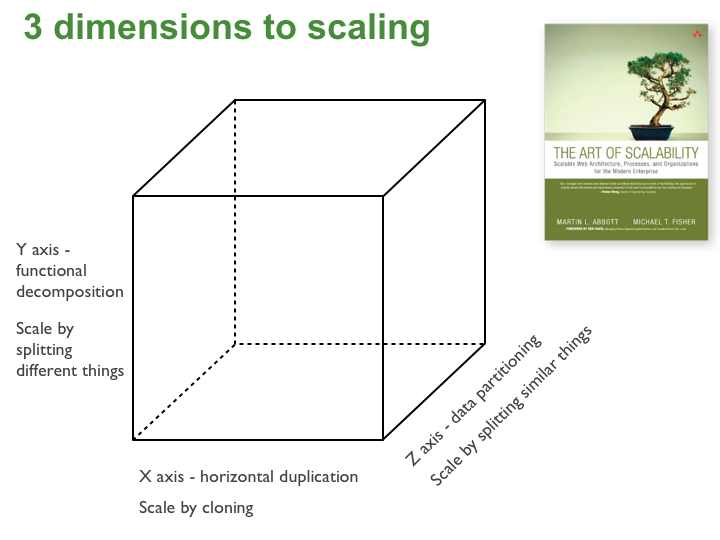
\includegraphics[width=\linewidth]{src/images/04-capitulo-4/scale_cube.jpg}
  \caption{El modelo de escalabilidad \eng{scale cube}}
  \label{fig:scale-cube}
\end{figure}

La arquitectura de servicios debe ser replicable y escalable. Para lograr esto cada \gls{acro:api} correrá en una instancia virtual independiente, de manera tal que la misma pueda ser replicada tantas veces como sea necesario (\eng{X-axis scaling}). El punto de acceso a esta arquitectura replicada será un balanceador de carga que servirá tanto para balancear la carga como \eng{failover}, dando continuidad a los servicios en caso de que alguna de las instancias replicadas fallen.

La característica fundamental de un balanceador de carga es ser capaz de distribuir las peticiones entrantes a un grupo de servidores (\eng{backends}) de acuerdo a un algoritmo de decisión y ponderación llamado \eng{scheduler}. Este algoritmo definirá cómo se toma la decisión de qué backend podría atender un requerimiento entrante, existiendo algunos simples (hacerlo de manera aleatoria o siguiendo un criterio ordenado por turnos como \eng{round robin}) y otros más sofisticados (que consideran otros factores como por ejemplo la carga de cada backend, su tiempo de respuesta promedio, el número de conexiones activas, la ubicación geográfica, etc.).

En su funcionamiento básico el balanceador de carga redirige las peticiones a alguno de los backends, el cual luego contesta al balanceador, para que finalmente sea el balanceador el que entregue la respuesta al cliente sin que este último sepa de la existencia de esta compleja arquitectura. Esta estructura transparente al cliente evita accesos directos entre éstos y los servidores que actúan como backend.

Como se mencionó anteriormente, el balanceador puede también ser usado como \eng{failover}, permitiendo que la falla de uno o más backends no afecten la disponibilidad del servicio. Los backends son monitoreados continuamente por el balanceador, cuando uno de estos falla el balanceador deja de enviar tráfico al backend caído. Luego cuando el backend vuelve a estar online el balanceador detecta esta situación y comienza a enviarle tráfico nuevamente.

Delante del balanceador se implementará una caché compartida utilizando \gls{db:varnish}, la misma evitará los accesos al balanceador, que puedan impactar de forma directa en alguna de las instancias replicadas de la \textit{API de Servicios} y \textit{API de Referencias}.

Según la RFC 7234\footnote{Este documento define las caches \gls{proto:http} y las cabeceras de control de cache permitidas en la versión \texttt{1.1} de ese protocolo\\\url{https://tools.ietf.org/html/rfc7234}}, una memoria cache almacena respuestas en pos de reducir el tiempo de respuesta y el consumo del ancho de banda. Asimismo, una memoria cache compartida es una cache que almacena respuestas para ser usadas por más de un usuario. Más adelante se tratará en detalle el uso de caches compartidas.

Como bien se indicó anteriormente, una cache compartida evitará los accesos a cualquiera de las instancias, ya sea de la \textit{API de Referencias} o la \textit{API de Servicios}, obteniendo mejores tiempos de respuesta así como tolerancia a fallos. Por ejemplo, podemos pensar en una aplicación (\textit{cliente A}) que accede al servicio \url{/academic_units} de la \textit{API de Referencias}. La petición es atendida por la \textit{API de Referencias}, donde el servicio devuelve todas la Unidades Académicas activas. Si más tarde otra aplicación (\textit{cliente B}), consulta la \gls{acro:api} por las Unidades Académicas, accediendo también al servicio \url{/academic_units} de la \textit{API de Referencias}, terminará obteniendo el mismo listado de Unidades Académicas. Como se puede apreciar, tenemos dos accesos a la \textit{API de Referencias} con idénticas respuestas, ambas procesadas por completo por uno o más backends. Esta situación puede evitarse con la inclusión de una cache compartida entre los diferentes clientes, logrando mejorar los tiempos de respuesta ya que la \textit{API de Referencias} recibirá únicamente un acceso, debiendo acceder y procesar los datos una única vez ya que el resto de las peticiones serán obtenidas desde la cache compartida.


\subsubsection{Desacoplamiento}

Para lograr el desacoplamiento, se propone desarrollar una \textit{API de Referencias} en la cual se implementarán los servicios necesarios que permitirán el acceso a los datos de referencia desde las distintas aplicaciones. El acceso a la \gls{acro:api} estará restringido a las direcciones IP de las aplicaciones (clientes) y al uso de un token, que se utilizará para validar el acceso a los servicios. Esta funcionalidad no será necesario desarrollarla, ya que esta capa de seguridad se implementará mediante el \gls{acro:esb}.

Para la solución planteada podemos observar las siguientes ventajas:

\begin{itemize}
  \item \textbf{Escalabilidad:} permite escalar horizontalmente (\eng{X-axis scaling}), es decir, en el hipotético caso que la \textit{API de Referencias} sea accedida por muchas aplicaciones, la misma podría replicarse en varias instancias, evitando la sobrecarga de cualquiera de ellas, al mismo tiempo que serviría como \eng{failover}.

  \item \textbf{Administración centralizada:} se centraliza la administración de los datos de referencia, evitando que la duplicidad se propague en cada aplicación que necesite utilizarlos.

  \item \textbf{Mantenimiento centralizado:} cuando hablamos de mantenimiento nos referimos a mejoras en la \gls{acro:api}, como por ejemplo, implementación de nuevos servicios, arreglo de errores, etc. Tener una \textit{API de Referencias} totalmente desacoplada de las aplicaciones que generan los datos permite actualizarla de forma más sencilla, evitando parar momentáneamente otras aplicaciones.

  \item \textbf{Agilización en el desarrollo:} otra de las ventajas que presenta este esquema, es la agilización en el desarrollo de nuevas aplicaciones. Ya no será necesario desarrollar el módulo que administra los datos de referencia, los mismos estarán en la \textit{API de Referencias} y se accederán a través de servicios.  De esta manera, evitamos duplicar código fuente para implementar esta funcionalidad, al mismo tiempo que acortamos los tiempos de desarrollo.
\end{itemize}

En segunda instancia, se deberán escribir de nuevo todas las \glspl{acro:api} que se encuentran actualmente en producción, esto es lo que llamaremos \textit{API de Servicios}. Para tal propósito, se utilizará el lenguaje de programación Ruby con el framework \nameref{soa:tecnologias:rails}, por los motivos que ya hemos expuesto en la \autoref{soa:tecnologias:para-servicios}. Esto dará origen a diferentes \textit{API de servicios}, que antes se encontraban implementados dentro de cada aplicación y acopladas a la misma, y ahora estarán implementados en una instancia virtual independiente.

De esta manera desacoplamos la lógica de la aplicación del acceso a los datos que se generan en la misma, permitiendo que esta solución escale horizontalmente, al igual que la \textit{API de Referencias}.

También se debe que tener en cuenta que esta solución permite independizarse del lenguaje en el que se desarrolló la aplicación: podemos desarrollar las aplicaciones en Ruby, PHP, JavaScript, Java o cualquier lenguaje, y la \gls{acro:api} separada en Ruby. Esto genera una capa de servicios en gran parte independiente de las aplicaciones, cuya única dependencia radica en el modelo de datos de cada aplicación, ya que si se modifica el modelo de la aplicación se deberá modificar de manera acorde el acceso a los datos, es decir los servicios.


\subsubsection{Simplicidad}

Es más simple que el anterior porque...

minimizar el costo del mantenimiento, desarrollo, testing, al mismo tiempo que se simplifica el deployment de los distintos entornos (desarrollo, testing y producción)

\subsubsection{Fault Tolerance}

Los sistemas distribuidos tienen potencialmente más fallos que los sistemas monolíticos, ya que en cada solicitud intervienen decenas (o cientos) de microservicios diferentes\cite[p.~48]{stin2015}. Es por esto que no resulta suficiente descomponer un sistema en componentes independientes; también hay que evitar que un fallo en uno de estos componenetes cause un fallo en cascada\cite[p.~4]{stin2015}.

Un fallo en cascada ocurre cuando un error en una capa interna provoca un fallo en la capa llamada\cite[p.~65]{nygard2007}. Mike Nygard describe en su libro ``Release It!''\cite{nygard2007} varios patrones tolerantes a fallos, de los cuales el mas popular es el \eng{Circuit Breaker}.

\begin{figure}[H]
  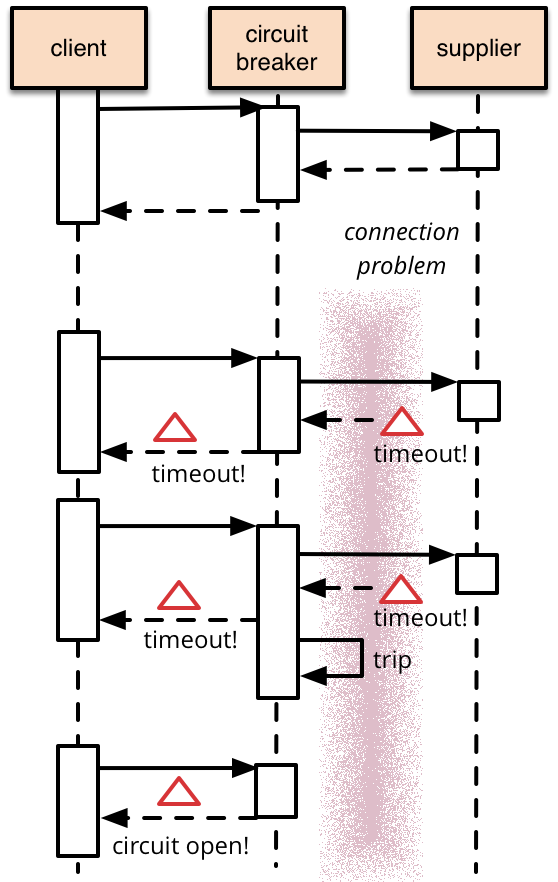
\includegraphics[width=\linewidth]{src/images/04-capitulo-4/circuit_breaker.png}
  \caption{Patrón de tolerancia a fallos \eng{Circuit Breaker}}
  \label{fig:circuit_breaker}
\end{figure}

Para implementar una infraestructura de servicios tolerante a fallos, los servicios estarán replicados en varias instancias virtuales y, como detallamos antes, delante de éstas se implementará un balanceador de carga, al mismo tiempo que se deberá trabajar en limitar el alcance de un fallo a nivel de servicio.

% ver si no es necesario sumar algo con respecto a los clientes

\subsubsection{Estandarización}

Según el diccionario de la Real Academia Española, un estándar es lo que sirve como tipo, modelo, norma, patrón o referencia. En nuestro caso, la estandarización es el proceso por el cual se establecen normas comunmente aceptadas que permiten la comunicación de diferentes aplicaciones.

Como mencionamos anteriormente, para cada aplicación que lo requiera se deberá implementar una \gls{acro:api} de acceso a datos propios generados localmente. Esta implementación se realizará basándose en la especificación \nameref{soa:tecnologias:json-api} detallada en la \autoref{soa:tecnologias:para-estructura}.

Esta estandarización facilitará el desarrollo de clientes que consuman información de los diferentes servicios de las \glspl{acro:api}, ya que definen con reglas que especifican cómo se podrá acceder a los datos, cuál será su estructura de respuesta, e incluso asisten en lograr independencia del lenguaje con el que se escriban estos clientes, quienes simplemente deben respetar las especificaciones para implementar el acceso a los servicios.


\newpage

  %   - Capítulo V
  \newpage
\section{Capítulo V: Caso testigo}
\label{cap5}

\todo{Escribir una breve introducción para este capítulo}

\textit{En este capítulo se documentan el caso testigo y el desarrollo del prototipo para ejemplificar. A partir de esto se debe desprender una conclusión. Posiblemente se enumeren acá los trabajos a futuro, principalmente la implementación efectiva del diseño que aquí planteamos.}

\subsection{Caso testigo}
\label{caso-testigo}

Habiendo desarrollado la propuesta de rediseño que motiva el presente trabajo, creemos conveniente tomar un caso testigo que sirva de ejemplo práctico para hacer concretos los conceptos teóricos que hemos tenido en cuenta para el análisis, a la vez que sirva de disparador para una implementación preliminar acotada del nuevo diseño sobre los elementos de la nube de servicios.

\subsubsection{Alcance}

La situación que utilizaremos como caso testigo, es el proceso de registro de un nuevo usuario de \gls{acro:sso} de la nube de servicios de la {\unlp}. Si bien \textit{a priori} puede parecer un tanto sencillo para tomarlo de referencia, una vez que definamos en concreto todos los pasos involucrados en este proceso se hará evidente la elección realizada.

Aquellos agentes que forman parte del personal de la UNLP pueden tener un usuario único para acceder a las aplicaciones que nuestro equipo desarrolla, ya sea para consultar sus recibos de haberes, utilizar una aplicación como parte de sus tareas diarias, presentar proyectos de extensión cuando la convocatoria se encuentre abierta o para acceder a cualquier aplicación que a futuro pudiéramos publicar. Para registrar su usuario, el agente dispone de dos vías:

\begin{itemize}
  \item La vía analógica: solicitando la creación del usuario, de manera presencial y por escrito, a la oficina de Personal de alguna de las Dependencias donde desempeña sus funciones. Por tratarse de un proceso manual y \eng{offline}, no lo consideraremos para este caso testigo.

  \item La vía digital: utilizando la \hyperref[anexo:detalle-clientes:sso]{aplicación de autogestión} que hemos desarrollado para realizar el registro en línea del nuevo usuario. \textit{Esta} es la vía que utilizaremos en nuestro planteo.
\end{itemize}

En el proceso de autogestión de un nuevo usuario, el agente debe completar los datos solicitados en una serie de pasos preestablecidos que lo guían hasta llegar a obtener el acceso a las aplicaciones que utilizan este esquema de \gls{acro:sso}\footnote{En realidad, inicialmente obtiene acceso únicamente a ver sus \hyperref[anexo:detalle-clientes:recibos]{recibos de haberes} y cargar su \textit{currículum de extensionista} en la aplicación de \hyperref[anexo:detalle-clientes:extension]{Proyectos de Extensión}. Para ingresar al resto de las aplicaciones un usuario autorizado le debe asignar los roles necesarios para cada aplicación. Para más información sobre las aplicaciones integradas al \gls{acro:sso} y la nube de servicios, referirse al \autoref{anexo:detalle-clientes}.}. Podemos resumir los pasos para el registro en:

\begin{enumerate}
  \item El agente ingresa a la aplicación de autogestión e indica que desea registrar un nuevo usuario. Para esto, debe ingresar una dirección de correo institucional propia para recibir por esa vía un vínculo de acceso para comenzar efectivamente el registro de su nuevo usuario.

  \item Al ingresar al vínculo de acceso que le llega a su correo, la aplicación solicita al agente que se identifique mediante su tipo y número de documento de identidad y en respuesta a ésto le indica si se encuentra entre los agentes de la Universidad que aún no tienen usuario de acceso único.

  \item Una vez identificado el agente, se le sugiere un nombre de usuario siguiendo la política de nombres de usuario, el cual puede ser modificado como parte de la carga de información que se está realizando. Se valida que este usuario esté disponible y que respete dicha política.

  \item Luego de elegido el nombre de usuario, se permite al agente ingresar una dirección de correo electrónico alternativa para tener un segundo medio de contacto.

  \item Para cerrar la carga de datos personales, se le pide que indique en qué Dependencias de la UNLP presta servicios. Esto se realiza por meido de un \gls{term:captcha} para evitar \eng{bots} que intenten registrar usuarios en masa y personas malintencionadas que deseen registrar usuarios en nombre de agentes reales.

  \item Al validar correctamente esta información, se le presentan todos los datos ingresados para su confirmación y si el agente los acepta, se le envía un correo electrónico con un formulario para presentar firmado en la oficina de Personal de alguna de las Dependencias donde presta servicios, teniendo un paso de validación humana de la información\footnote{Este paso adicional, si bien puede sonar contradictorio con el resto del proceso \eng{online} planteado, fue requerido por las autoridades de la Universidad para fortalecer los chequeos realizados sobre los datos recibidos mediante este servicio público de registro.}.

  \item Una vez presentado el formulario y debidamente corroborados los datos por algún empleado de la oficina de Personal correspondiente, el usuario es aprobado, evento que dispara el envío de un correo al agente, en el cual se le consignan su usuario y una clave provisoria para que ingrese por primera vez a los sistemas de la UNLP, y en ese momento la cambie por una clave de su propia elección. Con este paso, se finaliza el proceso de registro del nuevo usuario para el agente.
\end{enumerate}

Desde el punto de vista de nuestra aplicación, este proceso se ve un tanto reducido ya que no es necesario que incluyamos los pasos que ocurren por fuera del \textit{mundo virtual} o en la aplicación de gestión que utilizan los empleados de las oficinas de Personal de las Dependencias, ya que quedan fuera de su alcance. Formalizaremos los pasos que se realizan en este sistema con el diagrama de flujos presentado a continuación para su mejor comprensión.

\begin{figure}[H]
  \centering
  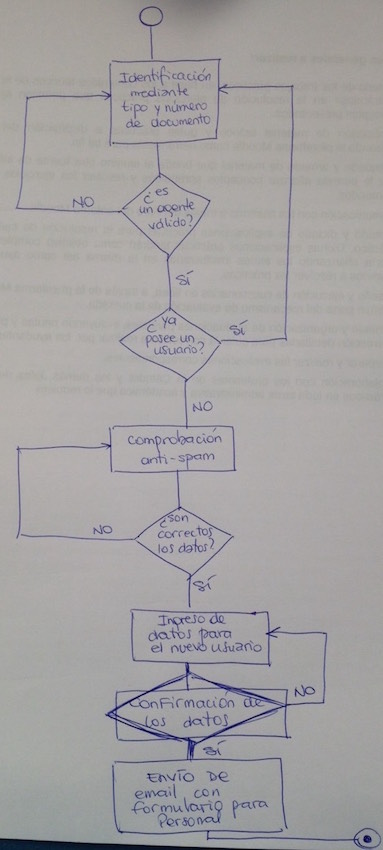
\includegraphics[width=\textwidth,height=0.5\textheight,keepaspectratio]{src/images/05-capitulo-5/diagrama-flujo-registro.jpg}
  \caption{Proceso de autoregistro de un nuevo usuario de acceso único}
  \label{fig:diagrama-flujo-registro}
\end{figure}

Realizando una descomposición en servicios del proceso anterior, identificamos las siguientes dependencias con servicios de la {\cloud}:

\begin{itemize}
  \item \textbf{Servicios de referencia:} para visualizar y marcar las Dependencias (o Unidades Académicas) y listados de tipos de documento de identidad.

  \item \textbf{Servicios de información sobre el personal:} en la identificación de la persona y posterior consulta de las Unidades Académicas en las cuales presta sus servicios.

  \item \textbf{Servicios de usuarios:} para la consulta de la existencia de un usuario de la persona seleccionada, sugerir nombres de usuario que respeten la política de nombres definida y en la creación del nuevo usuario.

  \item \textbf{Servicio de notificaciones:} en el envío de correos electrónicos. Destacamos en este punto que para limitar el alcance del caso testigo dejaremos la implementación de este servicio como un trabajo a futuro, ya que su existencia no es limitante para poder desarrollar los pasos de registro que se realizan en línea.
\end{itemize}

El desarrollo del prototipo funcional implica:

\begin{itemize}
  \item Implementar desde cero los servicios de la {\cloud} antes mencionados (de referencia, de información sobre el personal y de usuarios), en los cuales incluiremos únicamente los \eng{endpoints} necesarios para solventar la lógica del caso testigo.

  \item Implementar desde cero una nueva versión de la aplicación cliente de registro, respetando los pasos antes descriptos, que consuma toda la información de los servicios de la {\cloud}. Esta nueva versión difiere en su concepción de la versión actualmente implementada, en que no tendrá acceso a la base de datos de usuarios. De hecho, no tendrá acceso a \textit{ninguna} base de datos, ya que realizará todas sus operaciones de manera volátil dependiendo completamente de los servicios de la {\cloud} para acceder a la capa de persistencia en base de datos.

  \item Desarrollar una \textit{gema} (nombre que reciben las librerías reutilizables en el lenguaje Ruby) que encapsule la lógica de acceso a los servicios (cliente), desde la autenticación hasta la consulta y abstracción en objetos de las respuestas de sus \glspl{acro:api}, basándose en el estándar elegido para la codificación de la información.
\end{itemize}

Hemos elegido este caso testigo porque se compone de una serie de interacciones entre distintos servicios que brindan una noción de la complejidad que pueden tener las operaciones a realizar utilizando la nube de servicios, más allá de las simples consultas de datos de referencia que habitualmente manejamos. El hecho de incorporar diferentes servicios, englobados en distintas áreas de acción, nos permite también mostrar cómo funcionan las instancias de las aplicaciones que proveen esos servicios, cómo interactúan con la aplicación cliente y con los elementos intermediarios de la comunicación (entiéndase \eng{caches} compartidas, balanceadores de carga, \eng{proxies} reversos y la capa de mediación ofrecida por \nameref{soa:tecnologias:tyk}).

En este informe intentaremos no entrar en detalles innecesarios sobre la implementación de la aplicación cliente ni de la capa de lógica del negocio de los servicios, para sí ahondar sobre temas relevantes desde el punto de vista de la comprensión de las entidades participantes en las comunicaciones. Para su referencia, se adjunta al presente informe el código fuente de los distintos apartados que hemos implementado en este capítulo.


\subsubsection{Arquitectura}

Partiendo de la \autoref{propuesta}, el primer paso dentro de la implementación del prototipo funcional para este caso testigo es acotar la arquitectura, diseñarla y preparar los nodos en ella involucrados. Para esto, pueden observarse en la \autoref{fig:arquitectura-caso-testigo} los componentes lógicos del prototipo:

\begin{itemize}
  \item \textbf{Aplicación de registro:} esta es la implementación de una aplicación cliente de la {\cloud}. Es la cara visible hacia los usuarios públicos, y si bien en este caso particular hemos decidido implementarla utilizando \gls{fw:rails} por cuestiones prácticas, podría implementarse utilizando otras tecnologías como \eng{frameworks} web JavaScript que se ejecuten meramente del lado del cliente, PHP o Java, por nombrar algunas. De todos los componentes de la arquitectura, este es el único que se encuentra lógicamente por fuera de la {\cloud}. Esta separación del resto la hacemos evidente porque en este caso se trata de una aplicación desarrollada por nosotros mismos, pero en el futuro bien podría tratarse de una aplicación desarrollada por terceros, pertenecientes o no a la {\unlp}.

  \item \textbf{API Gateway (ESB):} este nodo se encarga de ser la capa que aisla los clientes de la \gls{acro:api}, brindando el acceso a los mismos desde un único punto. Como hemos visto con anterioridad, es el encargado de autorizar las peticiones entrantes y de chequear que se encuentren dentro de los límites para ellas establecidos, puede proveer una capa de caching intermedio, y también balancear la carga de los backends de servicios con un mecanismo de Round Robin que asigna una petición entrante \textit{no cacheada} a cada backend por vez. Complementariamente a estas tareas, el producto elegido en nuestro análisis para este rol (\nameref{soa:tecnologias:tyk}) provee una interfaz web de gestión para los usuarios internos que administran el acceso a los servicios (en principio, nosotros) con gráficos estadísticos del uso de nuestras \glspl{acro:api} que resulta de gran utilidad.

  \item \textbf{Cache de Gateway:} para obtener mejor rendimiento general de la {\cloud}, implementamos una Cache de Gateway ubicada por detrás del API Gateway. Esta capa adicional de caching nos permite evitar volver a procesar en los \eng{service components} peticiones que estén frescas en esa cache, incrementando la performance general de los servicios. Se encuentra implementada con \nameref{soa:tecnologias:varnish}, cache de alto rendimiento antes analizada y que hemos elegido para este rol.

  \item \textbf{Balanceador de carga:} para brindar la versatilidad de agregar o quitar tantas instancias de los \eng{service components} como se desee, incluimos un balanceador de carga antes de éstos para distribuir los requerimientos entrantes. Este se encuentra implementado con un \nameref{soa:tecnologias:nginx} que realiza la delegación de las peticiones mediante un Round Robin.

  \item \textbf{API de referencia:} esta, como el resto de las \glspl{acro:api} implementadas, provee un conjunto de servicios relacionados a una única incumbencia lógica, siguiendo el principio de una sola responsabilidad\footnote{También conocido como \eng{Single Responsibility Principle} en inglés. Este es uno de los cinco principios SOLID de diseño de software que apuntan a mejorar la calidad y facilidad del mantenimiento de un desarrollo.} e implementando el \hyperref[microservicios]{patrón de microservicios} tratado con anterioridad. En el caso de este \eng{service component}, su incumbencia es brindar los servicios de consulta de datos de referencia acotados a los necesarios para el alcance de este caso testigo: tipos de documento y unidades acdémicas. Se encuentra implementada con el framework \nameref{soa:tecnologias:rails} en su versión 5 en modo \texttt{--api}.

  \item \textbf{API de personal:} este nodo es otro \eng{service component} que se encarga de brindar los servicios relacionados a la información de personal de la {\unlp}. Esta es otra aplicación Rails versión 5 en modo \texttt{--api}.

  \item \textbf{API de usuarios:} otro \eng{service component} orientado a brindar acceso a las operaciones a realizar sobre los usuarios del esquema \gls{acro:sso}: gestión de usuarios y políticas de nombres de usuario. Al igual que en las \glspl{acro:api} anteriores, es una aplicación Rails 5 en modo \texttt{--api}.

  \item \textbf{API de notificaciones:} nodo que se dedica a la emisión de notificaciones (principalmente vía correo electrónico) que las aplicaciones cliente pudieran necesitar enviar. Es el \eng{service component} que en una aplicación monolítica sería reemplazado por el \eng{mailer} y el motor de generación de correos electrónicos. Similarmente a los casos anteriores, esta es otra aplicación Rails 5 en modo \texttt{--api}.

  \item \textbf{Capa de persistencia:} esta unidad de la arquitectura planteada es la encargada estrictamente del almacenamiento persistente de la información. Se trata de una base de datos MySQL, que pudiera estar replicada utilizando un modelo maestro-esclavo para conseguir redundancia y escalabilidad en el eje \textit{X}.

  \item \textbf{Cache compartida:} este componente de la arquitectura, de carácter opcional, beneficia en términos de escalabilidad y reducción de costos de procesamiento. Está implementado con un servidor de la base de datos clave-valor \gls{db:memcached}, que se utiliza como cache compartida entre las diferentes instancias de los \eng{service components} antes mencionados. Su principal función es evitar volver a calcular las respuestas que cualquiera de los servicios debiera brindar, si antes ya se la generó (ya sea en la misma instancia del servicio u otra distinta) y los datos originales no han cambiado.
\end{itemize}

Como demostración de las posibilidades de escalabilidad de esta arquitectura, hemos replicado los nodos de servicios para correr dos instancias de cada uno, las cuales serán balanceadas de manera transparente por \nameref{soa:tecnologias:nginx}.

\begin{figure}[H]
  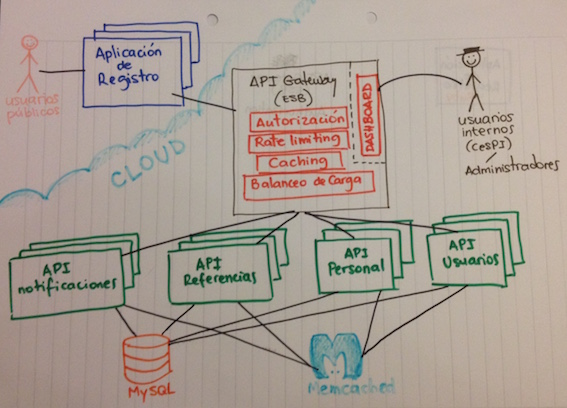
\includegraphics[width=\linewidth]{src/images/05-capitulo-5/arquitectura-caso-testigo.jpg}
  \caption{Visión lógica de la arquitectura del caso testigo}
  \label{fig:arquitectura-caso-testigo}
\end{figure}

\subsubsection{Desarrollo del prototipo funcional}

En el desarrollo de la arquitectura de nuestro caso testigo hemos seguido los principios que utilizamos en nuestra oficina de trabajo, tanto en la metodología ágil de desarrollo empleada, como en las herramientas fundamentales que se basan en productos \eng{Open Source}:

\begin{itemize}
  \item Para el versionado de nuestro código utilizamos el sistema de control de versiones \gls{scm:git}, con la interfaz web que brinda el producto GitLab\footnote{\url{https://about.gitlab.com}}.

  \item En el desarrollo usamos ambientes locales en nuestras computadoras, replicando un entorno similar a aquel en que finalmente vivirán las aplicaciones en producción.

  \item Para armar la topología de producción, utilizamos máquinas virtuales con tecnología openvz, sobre un entorno de virtualización basado en Proxmox\footnote{\url{http://www.proxmox.com/en/proxmox-ve}}, en el cual creamos libremente tantas instancias virtuales como necesitamos.

  \item Como sistema base de cada instancia virtual utilizamos una versión reducida de la distribución de GNU/Linux Ubuntu 14.04, que se encuentra modificada y simplificada para correr en máquinas virtuales consumiendo menos recursos.

  \item Para la resolución de los nombres de las instancias virtuales instalamos un servidor de DNS BIND9\footnote{\url{https://kb.isc.org/article/AA-01031}} utilizando el subdominios para cada host perteneciente a la zona \url{tesis.desarrollo.unlp.edu.ar}.

  \item Para aislar la arquitectura y evitar problemas de seguridad, utilizamos un esquema de red privada local al servidor de Proxmox, al cual accedimos mediante modificaciones a las tablas de \eng{routing} en nuestros equipos y la inclusión del servidor de DNS dedicado a la zona de nuestras instancias virtuales para la resolución de los nombres de cada equipo.

  \item Para los \eng{deployments} utilizamos Capistrano 3\footnote{\url{http://capistranorb.com}}, una herramienta altamente personalizable que automatiza los pasos necesarios para realizar la configuración, preparación, distribución y ejecución de cada una de nuestras aplicaciones (cliente y \glspl{acro:api}).

  \item Para la configuración de \nameref{soa:tecnologias:tyk} utilizamos \eng{Tyk Dashboard}, herramienta gratuita pero de código cerrado que distribuyen los creadores del API Gateway. En caso de no desear utilizar esa herramienta por no ser Software Libre podríamos utilizar la \gls{acro:api} REST que \nameref{soa:tecnologias:tyk} brinda para realizar esas configuraciones.  En este caso utilizamos la interfaz web para poder familiarizarnos con la configuración y gestión del producto de manera más sencilla.

  \item Para la implementación de los servicios siguiendo el estándar \nameref{soa:tecnologias:json-api} utilizamos una \textit{gema} que simplificó en varios órdenes de magnitud el desarrollo: \texttt{ActiveModelSerializers}\footnote{\url{https://github.com/rails-api/active_model_serializers}}. Esta gema brinda la lógica de presentación necesaria para estructurar las respuestas acorde a la especificación \nameref{soa:tecnologias:json-api} que elegimos para dar forma a las respuestas de la {\cloud}.

  \item Para la implementación de la lógica de acceso a los servicios de la {\cloud} desarrollamos una gema propia que reutilizamos en toda aquella aplicación que funcionaba como cliente, inclusive en las aplicaciones Rails que funcionaban como \gls{acro:api} y debían consumir información de otros servicios. Un ejemplo de esto último es el servicio de personas (parte de la \gls{acro:api} de personal), en el cual se hace referencia al tipo de documento de la persona, que se encuentra efectivamente en el servicio de tipos de documento que brinda la \gls{acro:api} de referencia. Del lado del servicio de personas, el tipo de documento se identifica a partir de su clave identificatoria, y cuando se necesita acceder a los atributos del tipo de documento (descripción o abreviatura) se realiza una petición como cliente del servicio de tipos de documento, pasando por el API Gateway como lo haría cualquier otro cliente.

  \item En la visual de la aplicación de Registro (la que funciona como cliente de la {\cloud}) utilizamos el framework CSS Bulma\footnote{\url{http://bulma.io}}, principalmente para diferenciar nuestro desarrollo como parte de este caso testigo de la estética institucional que mantienen los aplicativos desarrollados en el {\cespi}, que poseen un patrón visual común y utilizan el framework Bootstrap 3\footnote{\url{http://getbootstrap.com}}.
\end{itemize}

En el proceso de diseño de esta arquitectura decidimos acotar algunos aspectos planteados en la propuesta, principalmente para simplificar la arquitectura en nuestras pruebas, ya que no revestía un cambio significativo en el proceso de desarrollo pero sí nos insumiría tiempo de preparación, configuración y pruebas sobre los nuevos nodos introducidos. Como se mencionó antes, fue en ese sentido que dejamos sin implementar la \gls{acro:api} de notificaciones.

Si bien se podría haber simplificado aún más la arquitectura, la inclusión de los nodos de Cache de Gateway y balanceo de carga se debió a la búsqueda de escalabilidad sin necesidad de replicar la capacidad de procesamiento (es decir, evitando el procesaminto innecesario) y redundancia de nodos. Al utilizar \nameref{soa:tecnologias:varnish} detrás del API Gateway, podemos proveer una capa de caching de mayor rendimiento en comparación a la más modesta que provee \nameref{soa:tecnologias:tyk}. Luego, al incluir \nameref{soa:tecnologias:varnish} también podríamos utilizarlo para balancear la carga de los \eng{service components} ya que este producto lo admite, pero decidimos agregar un balanceador dedicado por detrás de la Cache de Gateway para tener un mecanismo de \eng{fallback} por si hubiera una caída del servicio de caching, en cuyo caso podríamos \textit{saltear} a \nameref{soa:tecnologias:varnish} hasta restablecer el servicio y utilizar directamente un \nameref{soa:tecnologias:nginx} como balanceador de carga, sin lógica de caching (la cual podría delegarse momentáneamente en \nameref{soa:tecnologias:tyk}).

\subsubsection{Experiencia}
\label{caso-testigo:experiencia}

A lo largo del desarrollo de las distintas partes involucradas en la implementación del caso testigo, pudimos apreciar cómo los conceptos clave enunciados hasta este punto en el informe se hacían presentes: desde la facilidad para realizar los \eng{deployments} virtualmente sin tiempo de caída del servicio, hasta la simplicidad introducida en el diseño y el desarrollo como producto de la clara separación de incumbencias por cada \eng{service component}.

A su vez, la libertad de gestionar los nodos de la arquitectura nos permitió experimentar con la cantidad y distribución de los mismos. Esto es extremadamente enriquecedor a la hora de comenzar a hacer pruebas sobre las posibles variantes de una arquitectura, ya que permite toparnos con eventuales problemáticas de su implementación efectiva.

Como resultado de esta experiencia fue gratificante confirmar que las elecciones de tecnologías que hicimos habían sido atinadas y altamente beneficiosas, entre otras cuestiones, porque:

\begin{itemize}
  \item \nameref{soa:tecnologias:rails} fue un medio muy veloz para tener de manera sencilla y ágil las aplicaciones completamente funcionales, implementando técnicas de caching altamente favorables para la performance general de las aplicaciones. Nuestros conocimientos de este framework hicieron que podamos tener en poco tiempo las primeras versiones de cada uno de los \eng{service components} y de la aplicación cliente.

  \item la adopción del estándar \nameref{soa:tecnologias:json-api}, tanto para la estructura de las respuestas de los servicios como para los mecanismos de realización de las peticiones, nos permitió utilizar gemas en ambos extremos de la comunicación que hicieron innecesaria la implementación de la lógica de conexión, transporte, serialización y des-serialización de la información.

  \item el uso de \nameref{soa:tecnologias:tyk} como API Gateway permitió que ignoremos detalles de autenticación y limitación por uso de recursos (\eng{rate limiting}) al implementar nuestros servicios. Adicionalmente, obtuvimos beneficios agregados como poder realizar balanceo de carga de las instancias de las \glspl{acro:api} con una configuración extremadamente sencilla, la gestión centralizada de claves de acceso, la recolección y visualización de datos estadísticos y analíticos del uso de los diferentes endpoints, y el chequeo de \eng{uptime} (tiempo en que el servicio se encuentra activo y funcionando correctamente) de las \glspl{acro:api}.

  \item como parte del desarrollo, unificamos los criterios base para las aplicaciones que funcionarían como \eng{service component}, creando una plantilla de aplicación en modo \gls{acro:api} como punto de partida al iniciar el desarrollo de este tipo de aplicaciones Rails.
\end{itemize}

\subsubsection{Resultado}

A continuación presentamos algunas capturas de pantalla en las que se pueden apreciar los distintos pasos implementados para la aplicación testigo de Registro de un nuevo usuario \gls{acro:sso} de la {\unlp}. Estos pasos pueden considerarse la implementación concreta del flujo expuesto anteriormente en la \autoref{fig:diagrama-flujo-registro} de este mismo capítulo.

En primer lugar, el usuario accede al sitio de registro, donde posibilita registrarse o acceder con su usuario y contraseña. Por ser el caso que nos atañe, seguiremos el camino del registro en las próximas capturas. En la \autoref{fig:caso-testigo:captura-000} podemos apreciar una captura de esta página.

\begin{figure}
  \centering
  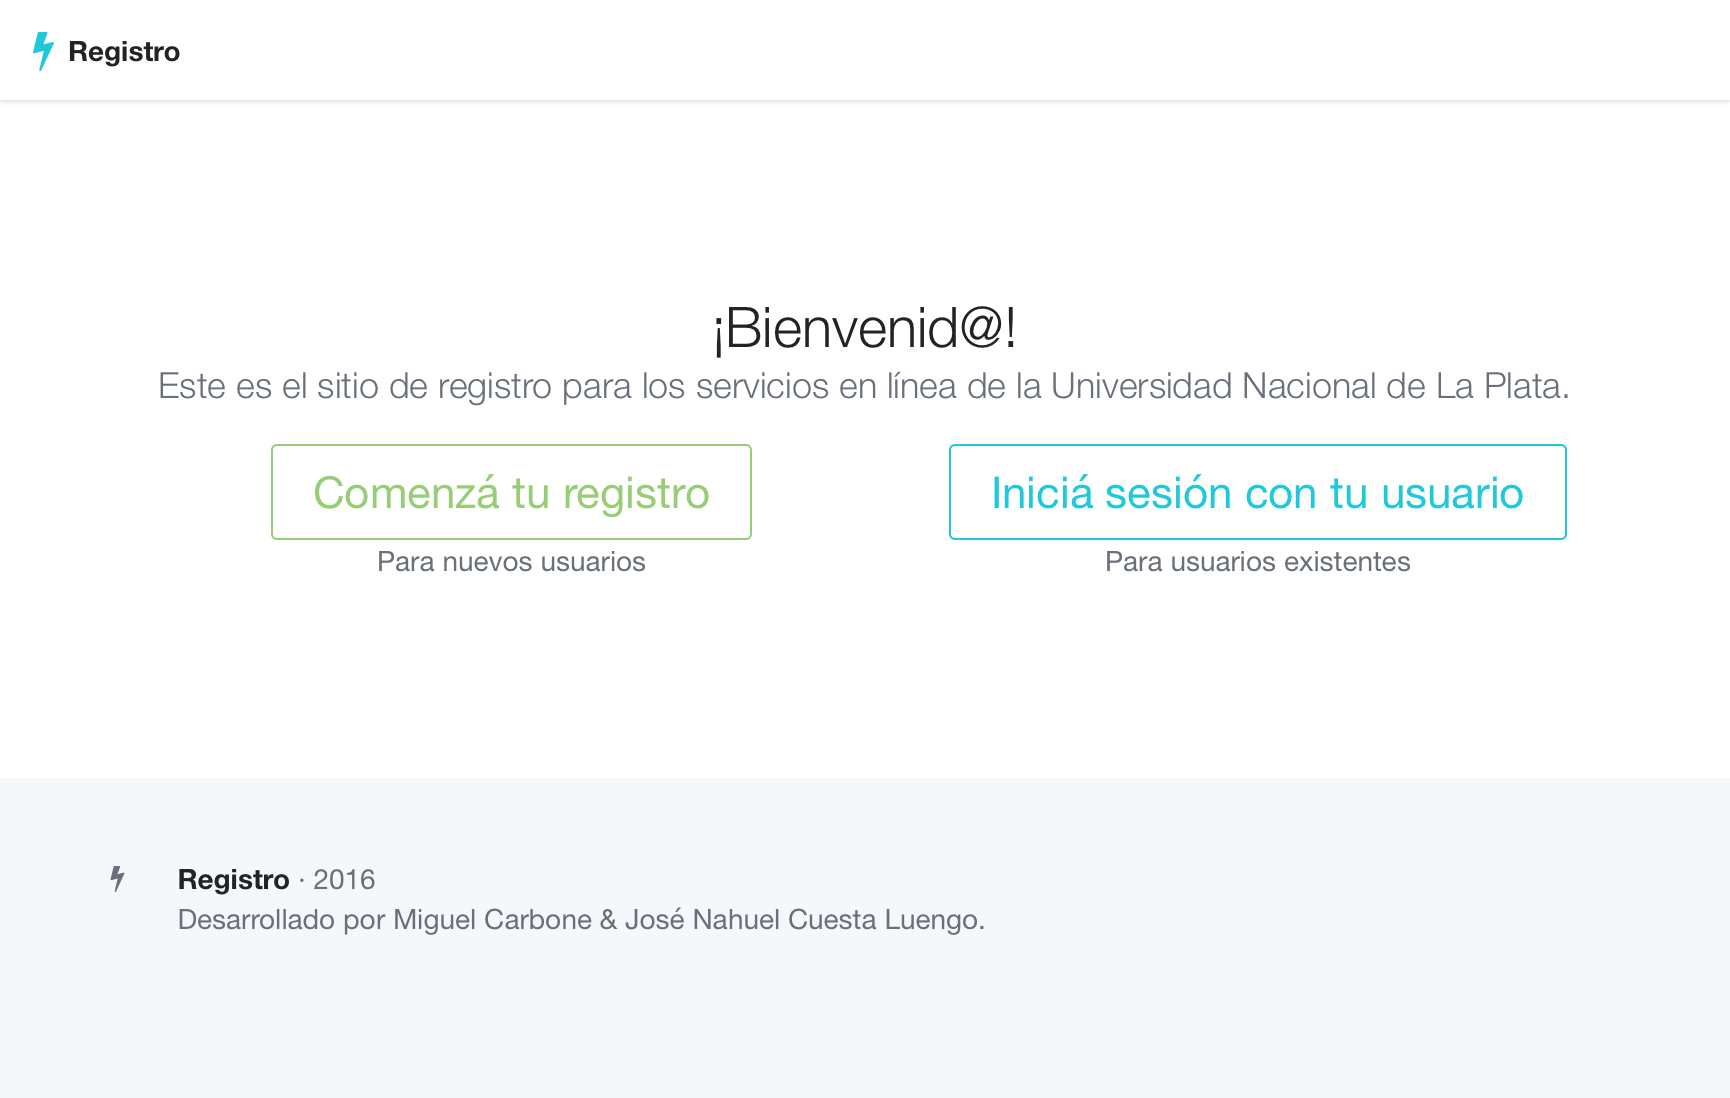
\includegraphics[width=\textwidth,keepaspectratio]{src/images/05-capitulo-5/capturas/page_000.png}
  \caption{Paso 0: bienvenida a la aplicación de Registro}
  \label{fig:caso-testigo:captura-000}
\end{figure}

En el paso siguiente, se solicita al interesado en registrarse que ingrese su correo personal e institucional. Este correo debiera ser una dirección válida, perteneciente a un dominio terminado en \texttt{unlp.edu.ar}.

\begin{figure}
  \centering
  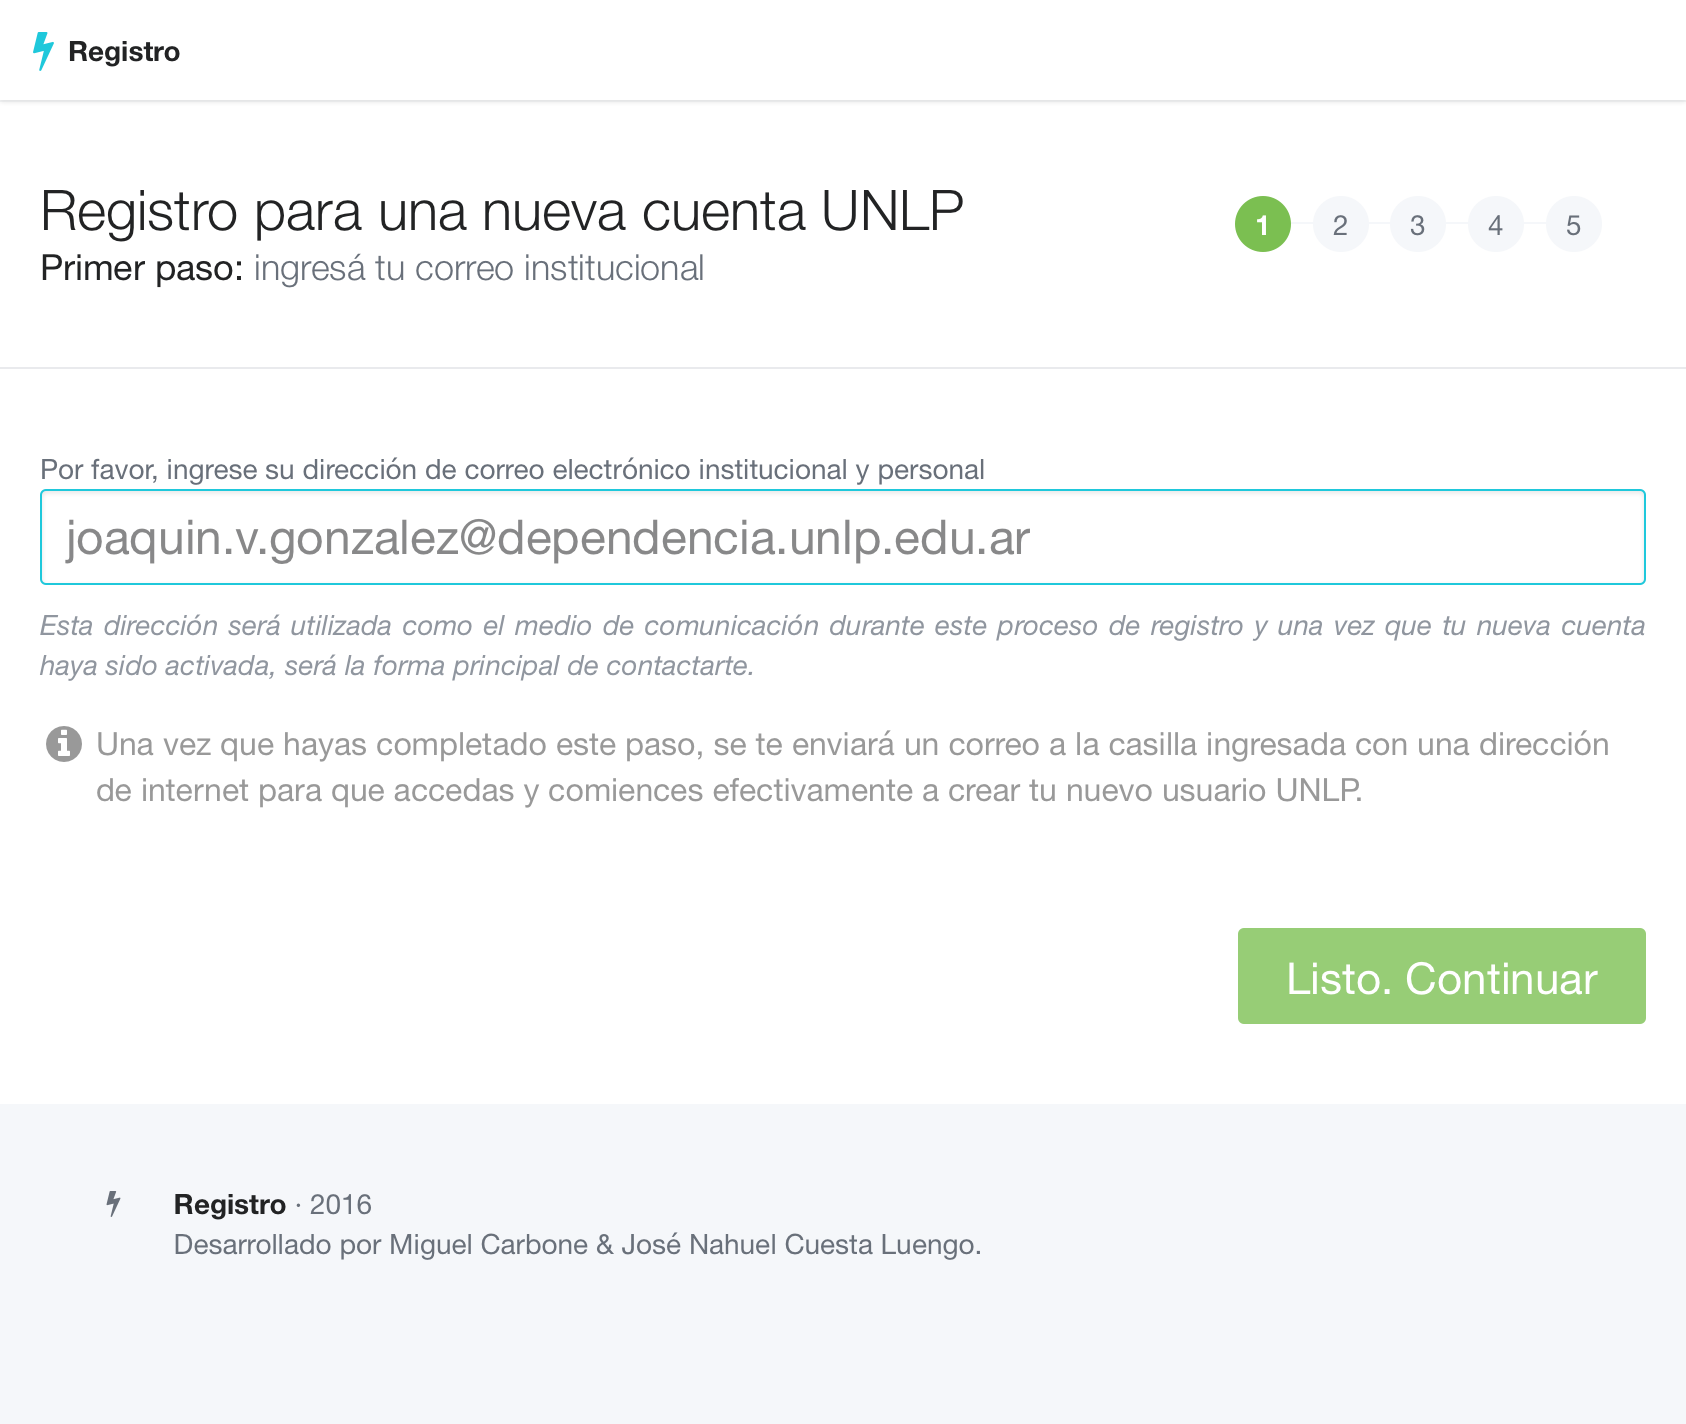
\includegraphics[width=\textwidth,keepaspectratio]{src/images/05-capitulo-5/capturas/page_001.png}
  \caption{Paso 1: inicio del registro}
  \label{fig:caso-testigo:captura-001}
\end{figure}

Una vez ingresado el correo electrónico, este es validado y en caso de cumplirse con los requerimientos antes expuestos, se le envía un correo electrónico a la dirección ingresada con un vínculo para continuar con el proceso de registro. Este paso es necesario para confirmar la dirección ingresada por el solicitante, puede apreciarse en la \autoref{fig:caso-testigo:captura-001}. En el momento en que se inicia el proceso de registro y justo antes de enviar el correo electrónico, se invoca al servicio de \eng{tókens} de la \gls{acro:api} de usuarios, el cual retorna un tóken con un código único\footnote{Más específicamente, utilizamos un \gls{term:uuid} como código único.} que es utilizado para generar una URL única para cada inicio de registro. Esos tókens tienen un tiempo de vida de una hora y pasado este período, debe generarse uno nuevo comenzando desde el principio el proceso de registro.

Por los motivos expuestos con anterioridad hemos decidido no implementar el servicio de notificaciones, por lo cual en la aplicación cliente implementada el usuario es llevado directamente al paso siguiente, tal como si hubiera recibido el correo electrónico y accedido al vínculo que habría en él.

\begin{figure}
  \centering
  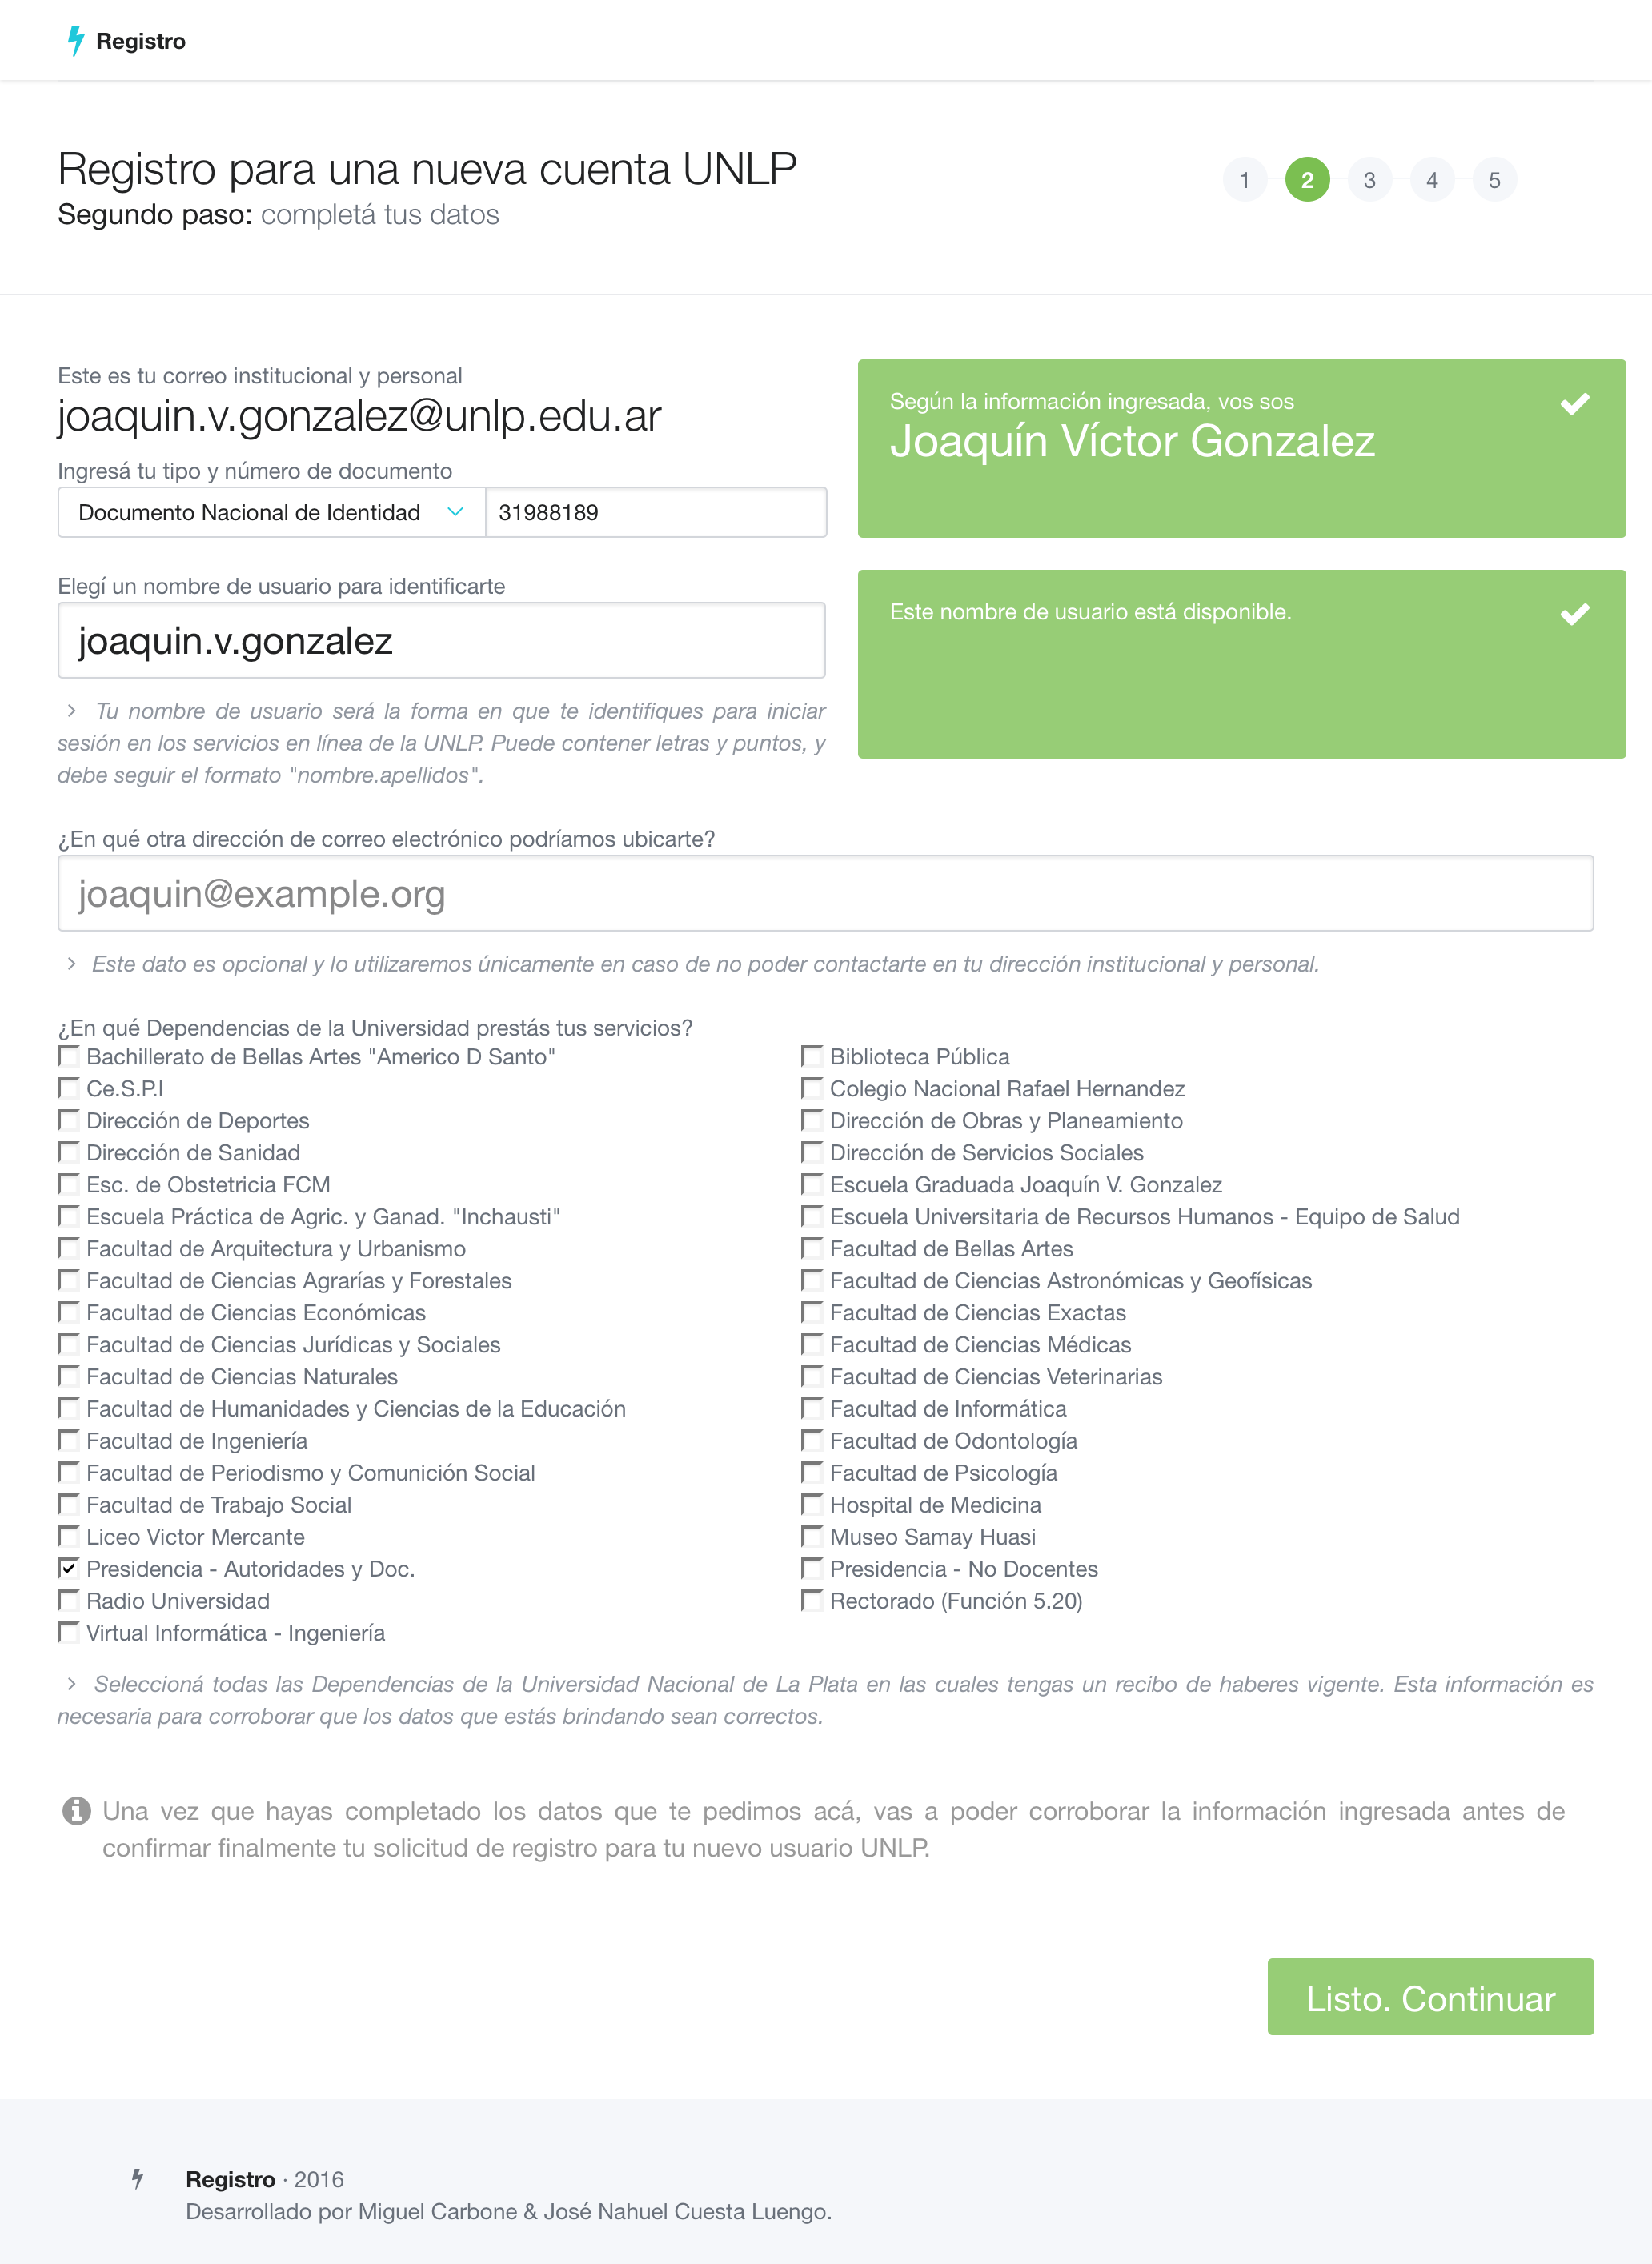
\includegraphics[width=\textwidth,keepaspectratio]{src/images/05-capitulo-5/capturas/page_002.png}
  \caption{Paso 2: identificación del nuevo usuario}
  \label{fig:caso-testigo:captura-002}
\end{figure}

En el paso siguiente, se presenta al usuario un formulario de carga de información para que se identifique, ingresando su tipo y número de documento, lo cual dispara una consulta asíncrona mediante AJAX a la \gls{acro:api} de personas y muestra la información acorde a los datos ingresados (pudiendo mostrarse el nombre de la persona en caso exitoso o un indicador de que la persona no es un agente de la UNLP). Si los datos se corresponden con una persona que no posea un usuario, se iniciará una segunda consulta asíncrona al servicio de nombres de usuario de la misma \gls{acro:api} para que sugiera un usuario válido acorde a la política de nombres de usuario a partir del nombre y apellido de la persona identificada. Finalmente se solicita un correo electrónico alternativo y que se indiquen las Dependencias en las que el solicitante presta servicios, a modo de \eng{captcha} para confirmar que se trate de un registro legítimo. Este paso puede observarse en la \autoref{fig:caso-testigo:captura-002}.

\begin{figure}
  \centering
  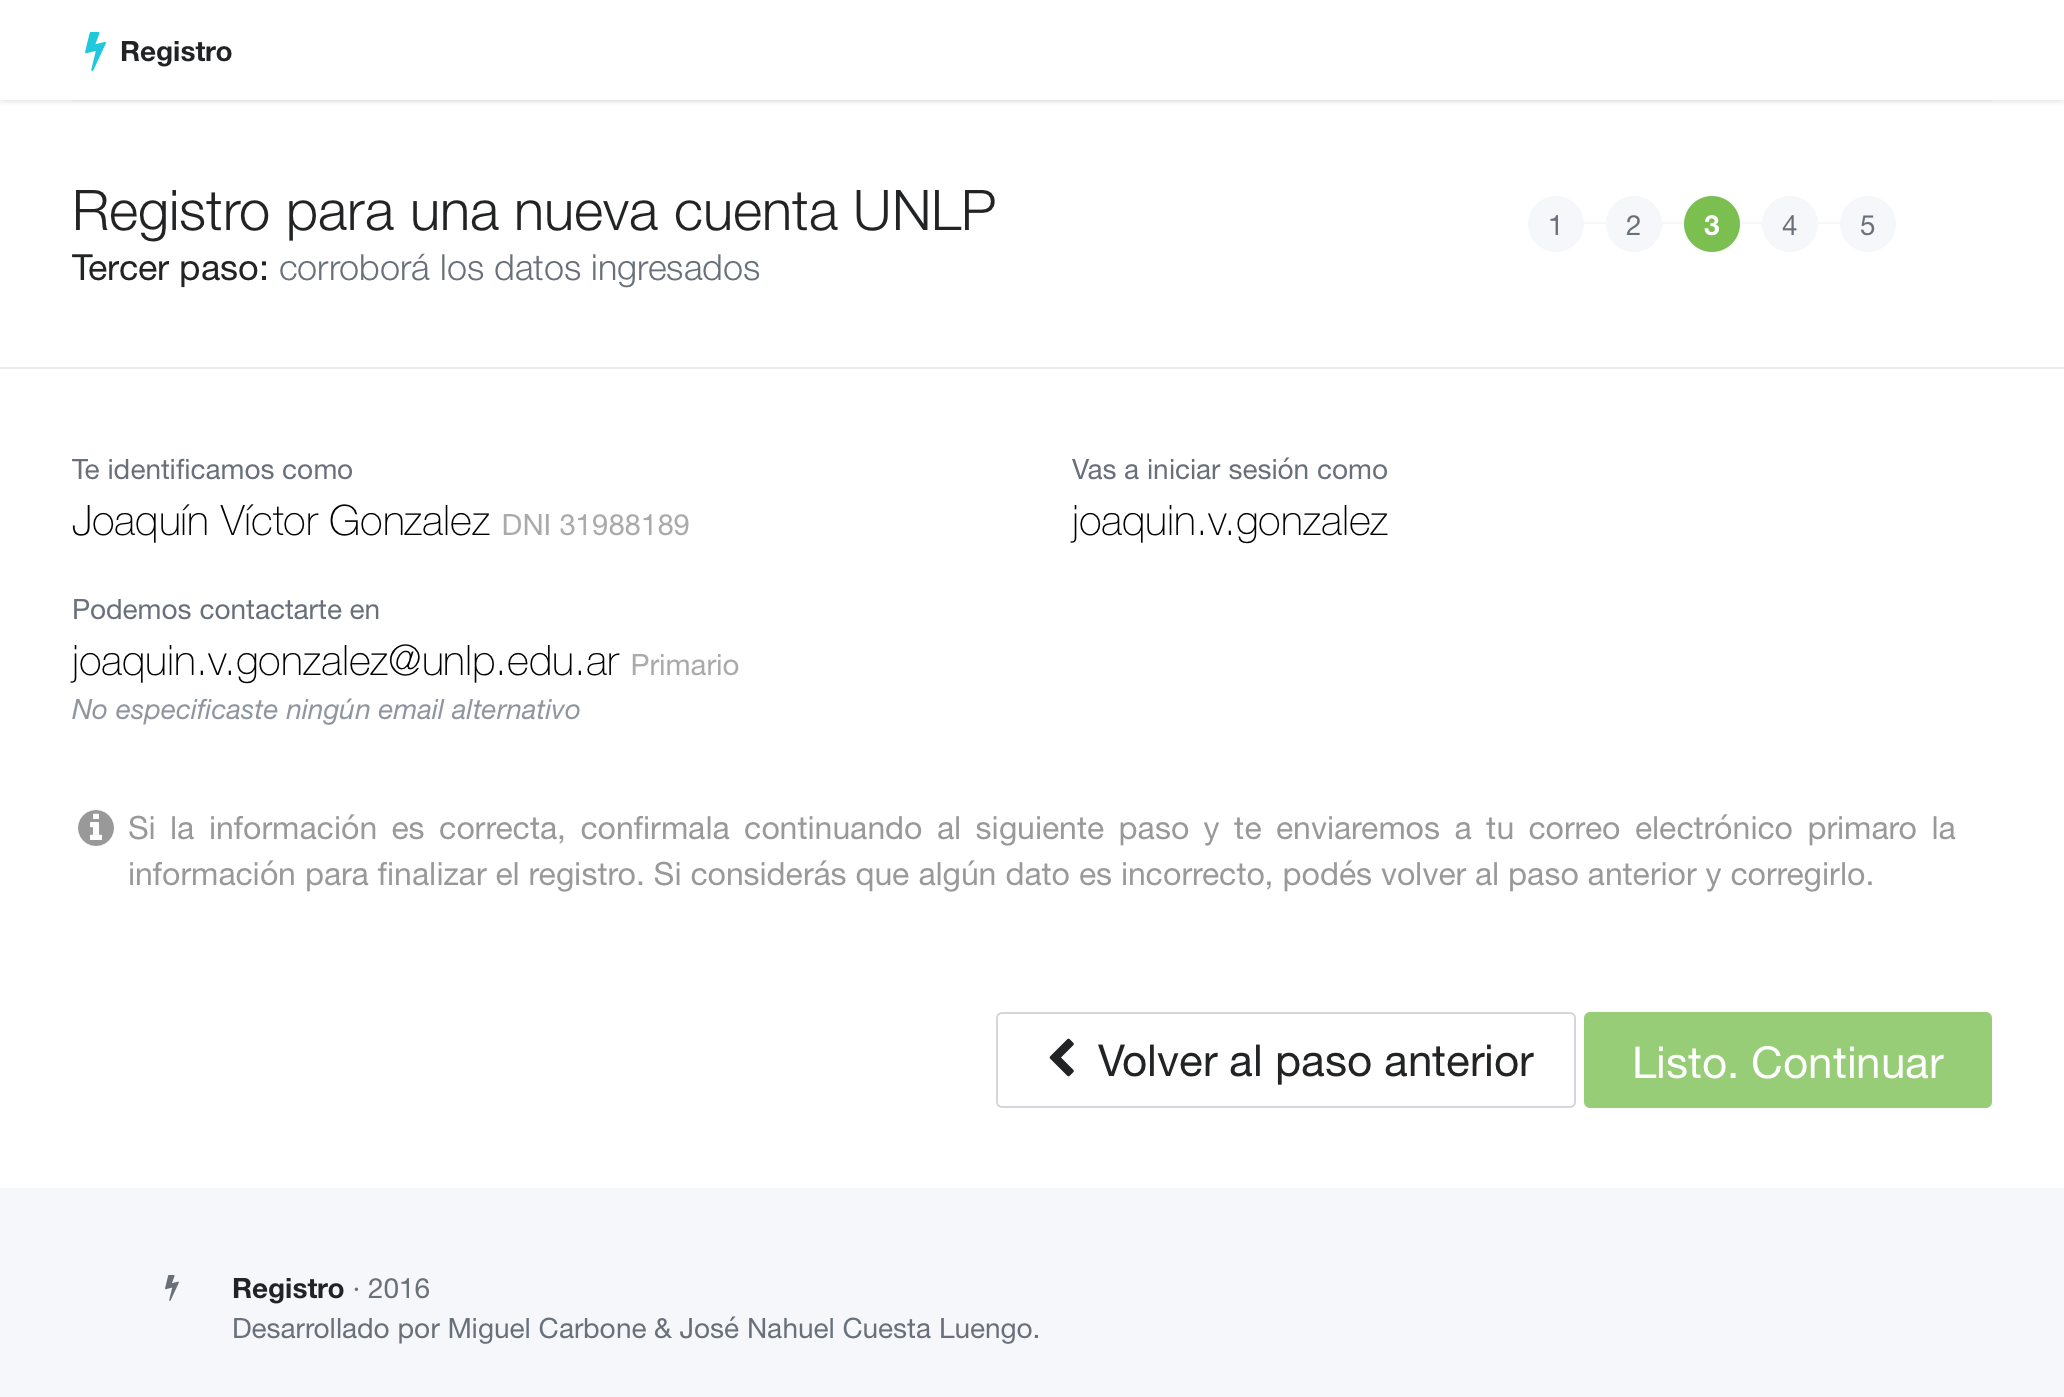
\includegraphics[width=\textwidth,keepaspectratio]{src/images/05-capitulo-5/capturas/page_003.png}
  \caption{Paso 3: confirmación de los datos}
  \label{fig:caso-testigo:captura-003}
\end{figure}

Por último, se presentan los datos ingresados para que el solicitante los confirme y genere efectivamente el nuevo usuario de \gls{acro:sso}, como puede verse en la \autoref{fig:caso-testigo:captura-003}. En caso de encontrar inconsistencias, puede optar por volver al paso anterior y corregirlas. Una vez confirmados los datos, se le enviará un correo mediante la \gls{acro:api} de notificaciones con los datos de la transacción y el formulario que deberá acercar personalmente a la oficina de Personal de su Dependencia. Adicionalmente, se hará un llamado al servicio de creación de usuarios de la \gls{acro:api} de usuarios para persistir la información, dejando el nuevo usuario en estado \textit{pendiente de aprobación}, para que sea aprobado por los agentes de la oficina antes mencionada cuando reciban el formulario de solicitud firmado por el solicitante. De esta manera se concluiría el circuito de registro que hemos tomado como caso testigo.


\clearpage
  %   - Capítulo VI
  \newpage
\section{Capítulo VI: Conclusión y trabajos futuros}
\label{cap6}

En este capítulo final, escribiremos las conclusiones obtenidas del análisis y desarrollo que hemos realizado como parte de esta elaboración. Basándonos en lo investigado en el marco teórico sentado en el capítulo II, en las alternativas tecnológicas comparadas en el capítulo III, y en las decisiones prácticas y concretas tomadas en los capítulos IV y V, es en este apartado que recogemos los frutos producto de nuestro trabajo.

Luego de la conclusión, terminaremos por enumerar los trabajos futuros que dejamos planteados para continuar, ya en conjunto con el resto del equipo de trabajo de la {\direccionDesarrollo}, hasta llegar a implementar y llevar a producción la nueva arquitectura para la nube de servicios de la UNLP, el resultado final de esta tesina.

\subsection{Conclusión}
\label{conclusion}

Comenzamos esta tesina a partir de la existencia de una problemática que necesitaba ser abordada desde distintos aspectos: el teórico, el cual nos daría bases firmes sobre las cuales plantear un nuevo diseño de la arquitectura de la nube, y el práctico, en el cual aplicaríamos los nuevos conocimientos adquiridos y adoptaríamos técnicas y tecnologías modernas para plantear un caso testigo.

Durante el proceso de investigación del estado del arte en la materia, nuestro enfoque inicial fue modificándose a partir de la asimilación de nuevos conceptos. El mayor cambio que experimentó nuestra concepción de la nueva arquitectura fue al ahondar en los microservicios (\autoref{microservicios}), patrón que nos resultó natural y adecuado para la {\cloud} y su nuevo diseño. De manera similar, al conocer productos alternativos a los \glspl{acro:esb} (\autoref{esb:introduccion} y \autoref{soa:tecnologias:para-nodo-central}) que preliminarmente habíamos relevado vimos la posibilidad de usar productos específicamente diseñados para la gestión de \glspl{acro:api} de servicios, delegando en éstos tareas como la autenticación, limitación de uso de recursos, registro de eventos y accesos, y la administración de clientes y medios para su acceso a la información.

Al hacer la prueba de concepto, obtuvimos una noción palpable del costo aparejado a implementar los servicios siguiendo el patrón de microservicios y a llevar estos cambios a nuestras aplicaciones. Ese experimento le da un alto valor agregado a este trabajo, ya que al momento de estimar el tiempo y los recursos necesarios para plasmar este cambio en los desarrollos existentes y futuros de nuestro equipo, podremos referirnos a esta experiencia. Ése es un punto clave dentro del camino que nos falta transitar para llegar al ambiente de producción con la {\cloud}, proceso que deberemos abordar, ya fuera del marco del presente trabajo, con el resto de nuestro equipo para planificar la transición ordenada de las aplicaciones existentes a la nueva arquitectura.

Con la implementación de una porción de la nueva arquitectura también pudimos experimentar los beneficios del uso del \hyperref[microservicios]{patrón de microservicios}\cite[p.~27]{richards2015}. Los puntos más fuertes derivados del uso de este patrón fueron la agilidad obtenida para el desarrollo, la facilidad para realizar despliegues independientes de los servicios en el ambiente de producción y, por sobre todas las cosas, el alto grado de desacoplamiento que acaban por tener los servicios entre sí y con respecto a las aplicaciones que los utilizan. Al separar los servicios por alcance, no presenta dificultades respetar el principio de una sola responsabilidad; y al separar las aplicaciones de los servicios, centralizando la lógica de negocios en estos últimos, se simplifican las aplicaciones clientes y se eliminan los posibles puntos de duplicación de código que pudieran existir en caso de tener la misma lógica de negocios presente en más de una aplicación\footnote{Este tipo de situaciones no nos es ajena, ya que en la actualidad tenemos diferentes aplicaciones que tienen en común parte de su lógica de negocios y por eso acaban duplicando porciones de código, con el impacto negativo que esa repetición conlleva.}. Asimismo, la arquitectura se puede extender e incluir nuevos \eng{service components} de manera transparente y sencilla, también debido al uso de este patrón y a la disposición de un \eng{broker} que funciona de intermediario.

La arquitectura diseñada logra mejoras más allá de las que nos propusimos inicialmente, producto de la investigación y aplicación de conceptos que al momento de comenzar esta tesina desconocíamos, cuanto menos, formalmente.

Como hemos expuesto en el apartado \textit{\nameref{caso-testigo:experiencia}} del caso testigo (\autoref{caso-testigo:experiencia}), consideramos que la elección de tecnologías para llevar a la práctica el diseño teórico fue beneficiosa y acertada, y que el producto final palpable que hemos generado es un punto de partida concreto para transmitir lo aprendido en este trabajo.

Este trabajo nos deja una propuesta para la arquitectura de la nueva {\cloud} de la {\unlp} que posee las características presentadas a continuación.

\begin{itemize}
  \item \textbf{Redundante:} admite la inclusión de nodos replicados en los distintos roles sin necesidad de modificar su diseño \textit{lógico}.
  \item \textbf{Extensible:} permite de manera transparente y sencilla incluir nuevos servicios o quitar algunos existentes, todo sin más rodeos que configurar el \eng{broker} acorde.
  \item \textbf{Escalable:} puede crecer en las distintas dimensiones del modelo \eng{scale cube} (ver \autoref{propuesta:escalabilidad}) según sea necesario.
  \item \textbf{Configurable:} su concepción está basada en la aceptación del cambio, y a tal fin debe poder ser modificada (o configurada) ante necesidades cambiantes.
  \item \textbf{Orientada a la \eng{performance}:} la introducción de diversas capas de caching, el balanceo de la carga de procesamiento entre diferentes instancias redundantes de los nodos, y la reescritura de la librería cliente para adoptar los beneficios que los estándares y el \gls{proto:http} caching están enfocados en reducir los tiempos de procesamiento y respuesta de los servicios, lo cual resulta en un mejor rendimiento general de la {\cloud}.
  \item \textbf{Basada en tecnologías Open Source:} siguiendo nuestros principios de trabajo, orientamos la elección de las herramientas utilizadas en todas las capas de la {\cloud} a productos Open Source, utilizadas por un número enorme de empresas y organismos, y que poseen comunidades sólidas que los respaldan y mantienen.
  \item \textbf{Basada en estándares abiertos:} al emplear estándares como \nameref{soa:tecnologias:json-api} y \gls{proto:http} caching, resulta más sencilla la integración de nuestro \eng{stack} de tecnologías con otros productos, e inclusive nos permite aprovechar herramientas desarrolladas por terceros para esos estándares sin necesidad de realizar implementaciones \textit{ad hoc}.
  \item \textbf{Hecha a medida:} se origina y desarrolla con la {\cloud} en mente, lo cual la hace altamente específica para los casos de uso que tendrá. Así como se basa en análisis e investigaciones del estado del arte en la materia, también está planteada a partir del aprendizaje de nuestros propios errores.
  \item \textbf{Simple:} intentamos incluir la cantidad justa de nodos para cumplir los roles necesarios en el diseño, sin agregar capas innecesarias ni eliminar puntos posibles de expansión al quitar algún nodo que habilite la redundancia.
  \item \textbf{Desacoplada:} cada \eng{service component} es una unidad lógica encargada de un conjunto concreto de tareas, cuyas interdependencias se manejan a través del \eng{broker} y no de forma directa, lo cual acoplaría un servicio a otro.
  \item \textbf{Robusta:} gracias a la redundancia y el desacoplamiento antes mencionados, el uso del \eng{broker} intermedio y las tecnologías empleadas, que han sido extensamente probadas en ambientes de producción.
  \item \textbf{Testeable:} su diseño descompuesto en capas y unidades independientes permite fácilmente aislar partes de la arquitectura para realizar pruebas sobre ellas.
\end{itemize}

En el siguiente apartado se presentan algunas tareas derivadas de la presente tesina para su posterior tratamiento.

\subsection{Trabajos futuros}
\label{trabajos-a-futuro}

A partir del presente informe y las experiencias obtenidas, tanto a partir de la formalización teórica de los conceptos involucrados en el diseño de una arquitectura orientada a servicios, como al llevarlos a la práctica en un caso concreto, consideramos que los puntos presentados a continuación permitirían extender lo aquí desarrollado.

\subsubsection{Automatización de la documentación}

Si bien hemos analizado productos para documentar y mantener la documentación de las \glspl{acro:api} desarrolladas, notamos que sería altamente beneficioso definir un proceso automático de actualización y publicación de la documentación de las mismas que se inicie cada vez que se publique una nueva versión del código de los servicios.

Esto mantendría siempre actualizada la documentación de los servicios, que deberían estar publicadas en un portal para desarrolladores que sirva para los integrantes de nuestra Dirección y para cualquier otro interesado en consumir la información pública de la {\cloud} de la {\unlp}.

\subsubsection{Automatización de la arquitectura}

En nuestras pruebas, hemos manejado de manera manual la instalación y configuración de la arquitectura base que utilizamos. Si bien esto puede funcionar bien para un caso testigo como el que aquí hemos presentado, al momento de llevar una arquitectura completa a producción es conveniente tener una forma automatizada, documentada y replicable de poner en funcionamiento todos sus nodos, como pueden ser \eng{scripts} de provisionamiento de los servidores involucrados.

En la actualidad, existe una cantidad considerable de herramientas que asisten en esta tarea, como por ejemplo Chef\footnote{\url{https://www.chef.io}}, Ansible\footnote{\url{https://www.ansible.com}} o Puppet\footnote{\url{https://puppetlabs.com}}, por nombrar algunos.

Se deja planteada para el futuro la necesidad de implementar esto con alguna herramienta afin, sea alguna de las aquí mencionadas u otra.

\subsubsection{Extensión de la gema cliente desarrollada}

El desarrollo que realizamos para dar soporte a las necesidades de la {\cloud} en nuestro caso testigo está limitado a aquellos puntos que se necesitó implementar. Aunque esto es un buen punto de partida y la gema resultante es completamente funcional, su alcance no sería suficiente para la implementación completa de la nueva nube de servicios.

Queda para etapas posteriores al presente trabajo la tarea de completar la lógica presente en la gema, agregando soporte para los nuevos \glspl{term:endpoint} que pudieran surgir, así como funcionalidad que asista al desarrollo de las aplicaciones cliente que no hayan sido necesarias para nuestro caso testigo.

\subsubsection{Implementación de pruebas}

Una buena práctica a la hora de desarrollar software es mantener una batería de pruebas a realizar sobre el producto para cerciorarnos que su ejecución genera los resultados esperados, y para garantizar que durante la evolución y el mentenimiento del mismo no se modifiquen su lógica de manera que impacte negativamente en dichos resultados. En el desarrollo de nuestro caso testigo obviamos la implementación de ese tipo de pruebas, dejando esto como una deuda técnica a saldar cuando este diseño comenzase a pasarse a desarrollo real. Recomendamos la realización de pruebas de unidad dentro de cada \gls{acro:api}, y de pruebas de integración entre las \glspl{acro:api} y las aplicaciones cliente, para garantizar que ningún cambio realizado en cualquiera de las partes intervinentes en la arquitectura produzca efectos secundarios no deseados en el resto.



  % Apéndice
  \appendix
  \newpage
  %   - Anexo I: Detalle de las aplicaciones cliente de la nube
  \section{Anexo I}
\label{anexo:detalle-clientes}

\subsection{Aplicaciones cliente de la nube de servicios de la UNLP}

Como ya hemos mencionado antes, la nube de servicios de la {\unlp} es el almacén de datos de referencia y de dominio general de las aplicaciones de uso interno de la UNLP que desarrollamos en nuestra oficina. En esta sección daremos un marco más concreto en referencia a qué aplicaciones la utilizan de manera que el lector pueda comprender en detalle el alcance y las interacciones existentes que movilizan el rediseño motivo del presente trabajo.

Por último, detallaremos las dependencias existenes entre las distintas aplicaciones y la nube de servicios, indicando qué \glspl{acro:api} utiliza cada una.


\subsubsection{Albergue Universitario}
\label{anexo:detalle-clientes:albergue}

Esta aplicación permite la gestión administrativa, de personal y de alumnos alojados en el Albergue Universitario de la {\unlp}. Los usuarios del sistema son el personal administrativo, del comedor y de Guardia Edilicia que desempeñan sus tareas en esa institución, permitiéndoles manejar las entradas y salidas de los alumnos, planificar las comidas acorde a la cantidad de comensales, y llevar un registro detallado de las actividades que por reglamento deben realizar los alumnos como parte de la beca que les permite residir en el albergue.

Es una aplicación desarrollada en \gls{fw:rails} versión 3, que actualmente se encuentra en etapa de mantenimiento correctivo de errores.


\subsubsection{Asociador}
\label{anexo:detalle-clientes:asociador}

El Asociador de documentos es una aplicación desarrollada para el uso conjunto entre el área de Digitalización de documentos del {\cespi} y la Dirección de Salud de la {\unlp}. Su objetivo es permitir que ése área suba en formato PDF las carpetas médicas históricas que digitaliza y luego las asocie a los agentes de la {\unlp}, de modo tal que el personal de la Dirección de Salud pueda consultar en línea dichas carpetas sin necesidad de contar con una oficina llena de biblioratos con las carpetas médicas otorgadas en los últimos 20 años en soporte papel.

Esta aplicación está desarrollada en \gls{fw:rails} versión 3, y actualmente se encuentra en etapa de mantenimiento correctivo de errores.


\subsubsection{Becas UNLP}
\label{anexo:detalle-clientes:becas}

La aplicación de Becas de la {\unlp} posee dos partes principales: una pública donde los alumnos (y futuros alumnos) de la Universidad pueden identificarse y solicitar algunas de las becas que la Universidad ofrece, y una privada accesible por personal de la Dirección de Becas que les permite realizar la asignación de las becas acorde a un órden de mérito que calcula el sistema, habilitar o deshabilitar becas de entre la oferta existente y agregar nuevas para que sean publicadas.

Está desarrollada en \gls{fw:symfony} versión 1.4, y actualmente se encuentra en etapa de mantenimiento correctivo de errores con soporte para nuevos requerimientos.


\subsubsection{Libretas Sanitarias}
\label{anexo:detalle-clientes:libretas}

Permite al personal de la Dirección de Salud la gestión de la información referente a las libretas sanitarias de los alumnos de la {\unlp}, la obtención de turnos y la consulta del estado de los trámites relacionados.

Se encuentra implementada con el \eng{framework} \gls{fw:rails} versión 3, y en este momento se encuentra bajo proceso de \gls{term:refactor} y migración a \gls{fw:rails} versión 4.


\subsubsection{Licencias Médicas}
\label{anexo:detalle-clientes:licencias}

La Dirección de Salud de la UNLP utiliza este sistema para gestionar las solicitudes de carpetas médicas, el tratamiento de esas solicitudes y el seguimiento de las eventuales licencias otorgadas a partir de ellas o las juntas médicas que pudieran surgir.

Esta aplicación fue desarrollada en \gls{fw:symfony} versión 1.2, y se encuentra en etapa de mantenimiento correctivo de errores. Tenemos planificada para la segunda mitad del año 2016 una reescritura de la aplicación para actualizar su \eng{stack} y extender su funcionalidad para brindar mejor soporte a situaciones no previstas en la versión actual, como por ejemplo permitir que los agentes de la {\unlp} soliciten en línea sus licencias, en lugar de tener que presentar en papel o telefónicamente los pedidos.


\subsubsection{Programa ``Mejor Aire''}
\label{anexo:detalle-clientes:mejor-aire}

Aplicación que gestiona las inscripciones de agentes de la UNLP al programa ``Mejor Aire'', una iniciativa de la Universidad para ayudar a dejar de fumar. Los inscriptos al programa participan semanalmente de reuniones de grupo y tienen controles periódicos para hacer un seguimiento de su evolución en el proceso. Mediante esta aplicación, los profesionales que llevan adelante el programa organizan los turnos, la asistencia a las reuniones y registran los chequeos realizados a cada inscripto.

Este sistema fue desarrollado utilizando \gls{fw:symfony} 1.2, y actualmente se encuentra en etapa de mantenimiento correctivo de errores.


\subsubsection{Proyectos de Extensión}
\label{anexo:detalle-clientes:extension}

El sistema actual de gestión de Proyectos de Extensión de la {\unlp} es el resultado de dos iteraciones de análisis de requerimientos e implementación, a partir de las cuales se depuraron las necesidades reales que la Secretaría de Extensión Universitario tenía para la versión \eng{on line} del proceso de presentación, acreditación, evaluación y adjudicación de los proyectos postulados para el programa de subsidio de proyectos de extensión de la Universidad Nacional de La Plata. La aplicación es utilizada por los directores y miembros de los proyectos para presentar sus propuestas, por los Secretarios de Extensión para avalar los proyectos presentados desde su Unidad Académica, por los integrantes de las comisiones evaluadoras para analizar y calificar las presentaciones, y por el personal de la Secretaría de Extensión para el otorgamiento final y seguimiento posterior de los proyectos subsidiados.

Este sistema fue reescrito en el año 2015, pasando de un desarrollo en \gls{fw:symfony} 1.1 a una aplicación totalmente renovada y con mucha más funcionalidad implementada utilizando el \eng{framework} \gls{fw:rails} versión 4. Se encuentra en desarrollo activo.


\subsubsection{Recibos de sueldo}
\label{anexo:detalle-clientes:recibos}

La aplicación de Recibos de sueldo permite a los agentes de la {\unlp} acceder de manera cómoda y a todo momento a sus recibos de sueldo, con la posibilidad de descargarlos para utilizarlos a su conveniencia, sin necesidad de acercarse a la oficina de Personal de su Dependencia para obtenerlos.

Esta aplicación también fue reescrita por completo en el año 2015, proceso mediante el cual pasó de ser un sistema \gls{fw:symfony} 1.4 a uno desarrollado con \gls{fw:rails} versión 4. Se encuentra en etapa de mantenimiento correctivo de errores e implementación de nuevos requerimientos, en caso que surjan.


\subsubsection{Responsables}
\label{anexo:detalle-clientes:responsables}

Este sistema centraliza la información que la oficina de Responsables de la {\unlp} gestiona para el seguimiento y la rendición de cuentas sobre el destino dado a los fondos que la Universidad posee. Registra todos los gastos imputados a las distintas partidas presupuestarias, cerciorándose que no existan inconsistencias entre los montos otorgados, su destino y el uso efectivo de los mismos.

Fue desarrollada con \gls{fw:rails} versión 3, y en la actualidad se encuentra en etapa de mantenimiento correctivo de errores.


\subsubsection{Acceso Único (SSO)}
\label{anexo:detalle-clientes:sso}

En el año 2015 se implementó de manera global la centralización de cuentas de usuario de los agentes de la {\unlp} para las aplicaciones que nuestra {\direccionDesarrollo} realiza, haciendo que cada persona disponga de una única cuenta que le permita acceder a aquellas aplicaciones que utilice para su labor diaria, así como también a sus datos personales y recibos de sueldo. Este proceso comprendió la creación de más de 5000 cuentas de usuario, la implementación de un proceso de autoregistro para los agentes y capacitaciones para los agentes de las oficinas de Personal de cada Dependencia en su uso.

Es una aplicación desarrollada en tres partes, dos de gestión (una para autogestión de cada usuario) y otra de administración general de los datos de usuarios, permisos y aplicaciones utilizando \gls{fw:rails} versión 4 y otra que implementa el estándar \gls{acro:saml} para proveer autenticación y autorización al resto de las aplicaciones. Se encuentra en mantenimiento correctivo de errores, con una planificación para extender su funcionalidad en el año 2016.


\subsubsection{Sueldos}
\label{anexo:detalle-clientes:sueldos}

La aplicación de Sueldos de la UNLP es una reimplementación completa del sistema que actualmente se encuentra en uso para liquidar los sueldos de la Universidad. Como aplicación, además de realizar el cálculo de la liquidación de sueldos, es el puntapié inicial para un sistema integral de gestión de recursos humanos de la {\unlp}. Este proyecto lleva alrededor de dos años en desarrollo y está planificado para ser puesto en producción en la primer mitad del año 2016.

Esta aplicación está desarrollada en \gls{fw:rails} versión 4, y se encuentra en desarrollo activo.


\subsubsection{Títulos}
\label{anexo:detalle-clientes:titulos}

Aplicación desarrollada para la Oficina de Títulos que digitaliza el proceso de solicitud de los títulos otorgados por la {\unlp} a sus alumnos, comprendiendo todas las etapas involucradas en el mismo desde la solicitud inicial hasta la entrega final del título en papel.

Este sistema fue desarrollado utilizando \gls{fw:rails} 3, se encuentra en mantenimiento correctivo de errores. Se tiene planificada su reescritura para el año 2016 debido a recientes cambios en el alcance inicialmente definido.


\subsubsection{Dependencias con la nube de servicios}
\label{anexo:detalle-clientes:dependencias-nube}

A continuación se presenta un cuadro que describe qué grupos de datos de los que provee la nube de servicios utilizan las aplicaciones enumeradas en este anexo.

En este cuadro se indica con un tilde ({\checkmark}) en qué grupos de \glspl{acro:api} depende cada aplicación, siendo los posibles grupos los siguientes:

\begin{itemize}
  \item \textbf{Ref} comprende las \glspl{acro:api} de datos de referencia.
  \item \textbf{Alumnos} abarca las \glspl{acro:api} de datos de alumnos de la UNLP.
  \item \textbf{Personal} referencia las \glspl{acro:api} de datos de agentes que trabajan en la {\unlp}.
  \item \textbf{Usuarios} indica que la aplicación usa las \glspl{acro:api} de datos de cuentas de usuarios registrados en el Sistema de Acceso Único.
\end{itemize}

\begin{table}[h!]
  %\begin{tabular*}{\textwidth}{ @{\extracolsep{\fill}} | p{0.4\textwidth} | m{0.15\textwidth} | m{0.15\textwidth} | m{0.15\textwidth} | m{0.15\textwidth} | }
  \begin{tabular*}{\textwidth}{ @{\extracolsep{\fill}} | p{0.39\textwidth} | c | c | c | c | }
    \hline
    \textbf{Aplicación}                           & \textbf{Ref} & \textbf{Alumnos} & \textbf{Personal} & \textbf{Usuarios} \\ \hline
    \nameref{anexo:detalle-clientes:albergue}     & {\checkmark} & {\checkmark}     &                   &                   \\ \hline
    \nameref{anexo:detalle-clientes:asociador}    & {\checkmark} &                  & {\checkmark}      &                   \\ \hline
    \nameref{anexo:detalle-clientes:becas}        & {\checkmark} & {\checkmark}     &                   &                   \\ \hline
    \nameref{anexo:detalle-clientes:libretas}     & {\checkmark} & {\checkmark}     &                   &                   \\ \hline
    \nameref{anexo:detalle-clientes:licencias}    & {\checkmark} &                  & {\checkmark}      &                   \\ \hline
    \nameref{anexo:detalle-clientes:mejor-aire}   & {\checkmark} &                  & {\checkmark}      &                   \\ \hline
    \nameref{anexo:detalle-clientes:extension}    & {\checkmark} & {\checkmark}     & {\checkmark}      & {\checkmark}        \\ \hline
    \nameref{anexo:detalle-clientes:recibos}      & {\checkmark} &                  & {\checkmark}      &                   \\ \hline
    \nameref{anexo:detalle-clientes:responsables} & {\checkmark} &                  &                   &                   \\ \hline
    \nameref{anexo:detalle-clientes:sso}          & {\checkmark} & {\checkmark}     & {\checkmark}      & {\checkmark}        \\ \hline
    \nameref{anexo:detalle-clientes:sueldos}      & {\checkmark} &                  & {\checkmark}      &                   \\ \hline
    \nameref{anexo:detalle-clientes:titulos}      & {\checkmark} & {\checkmark}     &                   &                   \\ \hline
  \end{tabular*}
  \caption{Dependencias de las aplicaciones con los servicios de la nube}
  \label{anexo:detalle-clientes:dependencias-nube:tabla}
\end{table}

\clearpage

  \newpage
  %   - Anexo II: Endpoints de la nube actual
  \section{Anexo II}
\label{anexo:endpoints-nube-actual}

\subsection{\eng{Endpoints} de la nube de servicios actual}

Aquí presentamos una lista de todos los \glspl{term:endpoint} de la nube de servicios de la UNLP tal como se encuentra al momento de escritura del presente trabajo. El propósito de este listado es mostrar las inconsistencias existentes en la forma de organizar las \glspl{acro:api} y la alta densidad de puntos de acción que provee la nube, de los cuales una gran parte no se encuentra en uso. Identificaremos los \glspl{term:endpoint} por los patrones de sus URLs (omitiremos el dominio y el protocolo para simplificar la lista):

\begingroup
  \begin{itemize}
    \item \lstinline$/api/academic_data.json/:id$
    \item \lstinline$/api/academic_degree_type.json$
    \item \lstinline$/api/academic_degree_type.json/:id$
    \item \lstinline$/api/academic_degree_type.json/count$
    \item \lstinline$/api/academic_unit.json$
    \item \lstinline$/api/academic_unit.json/:id$
    \item \lstinline$/api/academic_unit.json/count$
    \item \lstinline$/api/academic_unit/:id/academic_unit_college_degree.json$
    \item \lstinline$/api/academic_unit/:id/academic_unit_college_degree.json/count$
    \item \lstinline$/api/academic_unit/:id/career.json$
    \item \lstinline$/api/academic_unit/:id/career.json/count$
    \item \lstinline$/api/academic_unit/:id/career/:career_id/career_programme.json$
    \item \lstinline$/api/academic_unit/:id/career/:career_id/career_programme.json/count$
    \item \lstinline$/api/academic_unit/:id/career/:career_id/career_programme/:career_programme_id/career_programme_degree.json$
    \item \lstinline$/api/academic_unit/:id/career/:career_id/career_programme/:career_programme_id/career_programme_degree.json/count$
    \item \lstinline$/api/academic_unit/:id/career/:career_id/career_programme/:career_programme_id/career_subject.json$
    \item \lstinline$/api/academic_unit/:id/career/:career_id/career_programme/:career_programme_id/career_subject.json/count$
    \item \lstinline$/api/academic_unit/:id/degree.json$
    \item \lstinline$/api/academic_unit/:id/degree.json/count$
    \item \lstinline$/api/academic_unit/:id/degree/:degree_id/career_programme_degree.json$
    \item \lstinline$/api/academic_unit/:id/degree/:degree_id/career_programme_degree.json/count$
    \item \lstinline$/api/academic_unit/:id/paycheck.json$
    \item \lstinline$/api/academic_unit/:id/paycheck.json/count$
    \item \lstinline$/api/academic_unit/:id/paycheck.json/search/:query$
    \item \lstinline$/api/academic_unit/:id/paycheck.json/search/:query/count$
    \item \lstinline$/api/academic_unit/:id/person.json$
    \item \lstinline$/api/academic_unit/:id/person.json/count$
    \item \lstinline$/api/academic_unit/:id/person.json/search/:query$
    \item \lstinline$/api/academic_unit/:id/person.json/search/:query/count$
    \item \lstinline$/api/academic_unit_college_degree.json/:id$
    \item \lstinline$/api/career.json/:id$
    \item \lstinline$/api/career_programme.json/:id$
    \item \lstinline$/api/career_programme_degree.json/:id$
    \item \lstinline$/api/career_subject.json/:id$
    \item \lstinline$/api/census_data.json/:id$
    \item \lstinline$/api/city.json/:id$
    \item \lstinline$/api/country.json$
    \item \lstinline$/api/country.json/:id$
    \item \lstinline$/api/country.json/count$
    \item \lstinline$/api/country/:id/state.json$
    \item \lstinline$/api/country/:id/state.json/count$
    \item \lstinline$/api/country/:id/state/:state_id/department.json$
    \item \lstinline$/api/country/:id/state/:state_id/department.json/count$
    \item \lstinline$/api/country/:id/state/:state_id/department/:department_id/city.json$
    \item \lstinline$/api/country/:id/state/:state_id/department/:department_id/city.json/count$
    \item \lstinline$/api/degree.json/:id$
    \item \lstinline$/api/department.json/:id$
    \item \lstinline$/api/document_type.json$
    \item \lstinline$/api/document_type.json/:id$
    \item \lstinline$/api/document_type.json/count$
    \item \lstinline$/api/gender.json$
    \item \lstinline$/api/gender.json/:id$
    \item \lstinline$/api/gender.json/count$
    \item \lstinline$/api/marital_status.json$
    \item \lstinline$/api/marital_status.json/:id$
    \item \lstinline$/api/marital_status.json/count$
    \item \lstinline$/api/official_scale.json$
    \item \lstinline$/api/official_scale.json/:id$
    \item \lstinline$/api/official_scale.json/count$
    \item \lstinline$/api/official_scale/:id/personal_scale.json$
    \item \lstinline$/api/official_scale/:id/personal_scale.json/count$
    \item \lstinline$/api/paycheck.json/:id$
    \item \lstinline$/api/person.json$
    \item \lstinline$/api/person.json/:id$
    \item \lstinline$/api/person.json/count$
    \item \lstinline$/api/person.json/search/:id$
    \item \lstinline$/api/person/:id/academic_data.json$
    \item \lstinline$/api/person/:id/academic_data.json/count$
    \item \lstinline$/api/person/:id/academic_unit/:academic_unit_id/paycheck.json$
    \item \lstinline$/api/person/:id/academic_unit/:academic_unit_id/paycheck.json/count$
    \item \lstinline$/api/person/:id/academic_unit/:academic_unit_id/paycheck.json/search/:query$
    \item \lstinline$/api/person/:id/academic_unit/:academic_unit_id/paycheck.json/search/:query/count$
    \item \lstinline$/api/person/:id/census_data.json$
    \item \lstinline$/api/person/:id/census_data.json/count$
    \item \lstinline$/api/person/:id/is_graduated.json/:query_1/:query_2/:query_3$
    \item \lstinline$/api/person/:id/paycheck.json$
    \item \lstinline$/api/person/:id/paycheck.json/count$
    \item \lstinline$/api/person/:id/paycheck.json/search/:query$
    \item \lstinline$/api/person/:id/paycheck.json/search/:query/count$
    \item \lstinline$/api/person/:id/person_email.json$
    \item \lstinline$/api/person/:id/person_email.json/count$
    \item \lstinline$/api/person/:id/person_high_study.json$
    \item \lstinline$/api/person/:id/person_high_study.json/count$
    \item \lstinline$/api/person/:id/person_role.json$
    \item \lstinline$/api/person/:id/person_role.json/count$
    \item \lstinline$/api/person/:id/personal_age.json$
    \item \lstinline$/api/person/:id/personal_age.json/count$
    \item \lstinline$/api/person/:id/personal_charge.json$
    \item \lstinline$/api/person/:id/personal_charge.json/count$
    \item \lstinline$/api/person_email.json/:id$
    \item \lstinline$/api/person_high_study.json/:id$
    \item \lstinline$/api/person_role.json/:id$
    \item \lstinline$/api/personal_age.json/:id$
    \item \lstinline$/api/personal_charge.json/:id$
    \item \lstinline$/api/personal_scale.json/:id$
    \item \lstinline$/api/state.json/:id$
    \item \lstinline$/api/student_status.json$
    \item \lstinline$/api/student_status.json/:id$
    \item \lstinline$/api/student_status.json/count$
    \item \lstinline$/api/study_category.json$
    \item \lstinline$/api/study_category.json/:id$
    \item \lstinline$/api/study_category.json/count$
    \item \lstinline$/api/study_category/:id/study_type.json$
    \item \lstinline$/api/study_category/:id/study_type.json/count$
    \item \lstinline$/api/study_type.json/:id$
  \end{itemize}
\endgroup

  \newpage
  %   - Bibliografía
  \bibliographystyle{plain}
  \bibliography{src/bibliografia/mcarbone,src/bibliografia/ncuesta}
  \newpage
  %   - Glosario
  \printglossary[title={Glosario}]
  \newpage
  %   - Lista de figuras
  \listoffigures
  %   - Lista de bloques de código
  \listoflistings
  %   - Lista de tablas
  \listoftables
\end{document}
